\documentclass[book,chapter]{oblivoir}
\usepackage{kotex}
\usepackage{hyperref}
\usepackage{graphicx}
\usepackage{color}
\usepackage{verbatim}
\usepackage{amsmath}
\usepackage{amsfonts}
\usepackage{amssymb}
\usepackage{listings}
\usepackage{xcolor}
\usepackage{subfig}


% 기본 패키지 설정
\usepackage{lipsum} % 임시 텍스트 생성을 위한 패키지
\usepackage{kotex} % 한글 사용을 위한 패키지
\usepackage{graphicx} % 그림 삽입을 위한 패키지
\usepackage{titling} % 제목 스타일 변경을 위한 패키지
\usepackage{titlesec} % 챕터, 섹션 제목 스타일 변경을 위한 패키지
\usepackage{hyperref} % 하이퍼링크를 위한 패키지
\usepackage[dvipsnames]{xcolor} % 색상 사용을 위한 패키지
\usepackage{listings}
\usepackage[most]{tcolorbox}
\usepackage{float}
\usepackage{hyperref}
\usepackage{color}
\usepackage{verbatim}
\usepackage{amsmath}
\usepackage{amsfonts}
\usepackage{amssymb}
\usepackage{xcolor}
\usepackage{subfig}

\usepackage{tikz}
\usetikzlibrary{shapes.geometric, arrows}

\tikzstyle{startstop} = [rectangle, rounded corners, minimum width=3cm, minimum height=1cm,text centered, draw=black, fill=red!30]
\tikzstyle{process} = [rectangle, minimum width=3cm, minimum height=1cm, text centered, draw=black, fill=NavyBlue!30]
\tikzstyle{arrow} = [thick,->,>=stealth]


% Listings settings
\lstset{
  language=Python,
  basicstyle=\ttfamily\footnotesize,
  numbers=left,
  numberstyle=\tiny\color{gray},
  stepnumber=1,
  numbersep=5pt,
  backgroundcolor=\color{white},
  showspaces=false,
  showstringspaces=false,
  showtabs=false,
  frame=single,
  rulecolor=\color{black},
  tabsize=2,
  captionpos=b,
  breaklines=true,
  breakatwhitespace=true,
  escapeinside={\%*}{*)},
  keywordstyle=\color{blue},
  commentstyle=\color{gray},
  stringstyle=\color{red},
}


% Title page enhancements
\pretitle{\begin{center}\fontsize{40}{48}\bfseries\color{MidnightBlue}}
\posttitle{\end{center}}
\preauthor{\begin{center}\Large\mdseries\color{ForestGreen}}
\postauthor{\end{center}}
\predate{\begin{center}\Large\color{OrangeRed}}
\postdate{\end{center}}

% Part title styling
\titleformat{\part}
  {\fontsize{50}{48}\bfseries\color{Maroon}}
  {\thepart}
  {20pt}
  {\filcenter}

% Chapter title styling
\titleformat{\chapter}[display]
  {\bfseries\fontsize{40}{48}\selectfont\color{RoyalBlue}}
  {\filright\fontsize{40}{48}\selectfont\color{RoyalBlue} 제\ \thechapter\ 장}
  {20pt}
  {\filcenter}

% Section title styling
\titleformat{\section}
  {\LARGE\bfseries\color{Sepia}}
  {\thesection}
  {1em}
  {}

% Subsection title styling
\titleformat{\subsection}
  {\Large\bfseries\color{OliveGreen}}
  {\thesubsection}
  {1em}
  {}

% Subsubsection title styling
\titleformat{\subsubsection}
  {\Large\bfseries\color{NavyBlue}}
  {\thesubsubsection}
  {1em}
  {}

% Affiliation command
\makeatletter
\newcommand{\affiliation}[3]{%
  \gdef\@affiliation{#1}%
  \gdef\@name{#2}%
  \gdef\@contact{#3}}
\newcommand{\printaffiliation}{%
  \vfill
  \begin{center}
    \LARGE
    \textcolor{ForestGreen}{\@name} \\
    \href{mailto:\@contact}{\textcolor{MidnightBlue}{\@contact}} \\
    \textcolor{MidnightBlue}{\@affiliation}
  \end{center}}
\makeatother

% Define a new tcolorbox style called KnowledgeBox
\newtcolorbox[auto counter, number within=section]{KnowledgeBox}[2][]{
  colframe=teal!60!black, 
  colback=teal!10, 
%  title=지식상자 \thetcbcounter: #2, 
  title=지식상자: #2,
  fonttitle=\bfseries, 
  coltitle=white, 
  rounded corners, 
  enhanced, 
  boxrule=0.8mm, 
  float, % Enable floating behavior
  floatplacement=b, % Float box placement at the bottom of the page
  #1
}


% 페이지 배경색 설정\pagecolor{GreenYellow}

\lstset{
  basicstyle=\ttfamily,
  keywordstyle=\color{blue},
  commentstyle=\color{green},
  stringstyle=\color{red},
  numbers=left,
  numberstyle=\tiny\color{gray},
  stepnumber=1,
  numbersep=10pt,
  backgroundcolor=\color{lightgray!20},
  frame=single,
  breaklines=true,
  breakatwhitespace=false,
  showspaces=false,
  showstringspaces=false,
  showtabs=false,
  tabsize=2,
  captionpos=b,
}
% Define the Dockerfile language
\lstdefinelanguage{dockerfile}{
  keywords={FROM, RUN, CMD, LABEL, MAINTAINER, EXPOSE, ENV, ADD, COPY, ENTRYPOINT, VOLUME, USER, WORKDIR, ARG, ONBUILD},
  morecomment=[l]{\#},
  morestring=[b]",
  sensitive=true
}

\lstdefinelanguage{yaml}{
  keywords={true, false, null, y, n},
  basicstyle=\ttfamily\footnotesize,
  morecomment=[l]{\#},
  commentstyle=\color{gray},
  morestring=[b]',
  morestring=[b]",
  stringstyle=\color{blue},
  literate=
   *{0}{{{\color{numb}0}}}{1}
    {1}{{{\color{numb}1}}}{1}
    {2}{{{\color{numb}2}}}{1}
    {3}{{{\color{numb}3}}}{1}
    {4}{{{\color{numb}4}}}{1}
    {5}{{{\color{numb}5}}}{1}
    {6}{{{\color{numb}6}}}{1}
    {7}{{{\color{numb}7}}}{1}
    {8}{{{\color{numb}8}}}{1}
    {9}{{{\color{numb}9}}}{1}
    {:}{{{\color{punct}{:}}}}{1},
}

% Custom shell command language definition for Linux commands
\lstdefinelanguage{Shell}{
  keywords={cd, ls, mkdir, rm, rmdir, sudo, apt-get, yum, pacman, mv, cp, docker, run, build, stop, start, exec, ps, init, install, update, chmod, curl, tee, echo, uname, uptime, sh, dpkg, docker-ce, docker-ce-cli, containerd.io, docker-buildx-plugin, docker-compose-plugin},
  keywordstyle=\color{blue}\bfseries,
  sensitive=true,
  comment=[l]{\#},
  morecomment=[s]{/*}{*/},
  morestring=[b]",
  morestring=[b]',
  alsoletter={-},
}

\affiliation{국립목포대학교 컴퓨터공학과}{이영호}{youngho.lee@gmail.com}

\title{초보자를 위한 \\도커(Docker) 실습}
%\author{Prakhar Srivastav}
\date{\today}

\begin{document}

\maketitle
\printaffiliation
\chapter*{머리말}

이 문서는 Docker를 이해하고 사용하는 방법에 대한 튜토리얼입니다. Docker는 애플리케이션의 배포를 자동화하는 오픈 소스 프로젝트로, 컨테이너를 사용하여 소프트웨어 애플리케이션을 운영 체제 수준에서 가상화합니다. 이 문서는 Docker의 기본 개념, 설치 방법, 기본 명령어 사용법, 웹 애플리케이션의 Docker 이미지를 생성하고 배포하는 방법 등을 다룹니다. 이 튜토리얼을 통해 Docker의 이점을 이해하고, 실제 환경에서 Docker를 활용할 수 있는 능력을 갖추게 될 것입니다.

이 교재의 대부분의 내용은 https://docker-curriculum.com 에서 참조하였습니다. 감사합니다.

\newpage
\tableofcontents

\chapter{소개}
\section{Docker란 무엇인가요?}
Wikipedia는 \href{https://www.docker.com/}{Docker}를 다음과 같이 정의합니다:
\begin{quote}
    Docker is a set of platform as a service (PaaS) products that use OS-level virtualization to deliver software in packages called containers. The service has both free and premium tiers. The software that hosts the containers is called Docker Engine. It was first released in 2013 and is developed by Docker, Inc.

    Docker is a tool that is used to automate the deployment of applications in lightweight containers so that applications can work efficiently in different environments in isolation.

    Docker는 OS 수준 가상화를 사용하여 컨테이너라고 불리는 패키지 형태로 소프트웨어를 제공하는 플랫폼 서비스(PaaS) 제품군입니다. 이 서비스는 무료 및 프리미엄 등급을 모두 제공합니다. 컨테이너를 호스팅하는 소프트웨어는 Docker Engine이라고 불리며, 2013년에 처음 출시되었고 Docker, Inc.에서 개발했습니다.
    
    Docker는 애플리케이션을 가벼운 컨테이너에 배포하는 작업을 자동화하는 도구로, 애플리케이션이 서로 독립된 다양한 환경에서 효율적으로 작동할 수 있도록 합니다.
\end{quote}

Docker는 개발자, 시스템 관리자 등이 응용 프로그램을 호스트 운영 체제(즉, 리눅스)에서 실행할 수 있는 샌드박스(컨테이너라고 함)에 쉽게 배포할 수 있게 하는 도구입니다. Docker의 주요 이점은 응용 프로그램과 모든 종속성을 소프트웨어 개발을 위한 표준화된 단위로 패키징할 수 있다는 것입니다. 가상 머신과 달리 컨테이너는 높은 오버헤드가 없어서 기본 시스템 및 리소스를 보다 효율적으로 사용할 수 있습니다.

\section{컨테이너란 무엇인가요?}
오늘날 업계 표준은 소프트웨어 응용 프로그램을 실행하기 위해 가상 머신(VM)을 사용하는 것입니다. VM은 가상 하드웨어에서 실행되는 게스트 운영 체제 내부에서 응용 프로그램을 실행합니다.

VM은 응용 프로그램의 전체 프로세스를 격리하는 데 매우 유용합니다. 호스트 운영 체제의 문제가 게스트 운영 체제에서 실행되는 소프트웨어에 영향을 미칠 수 있는 방법은 거의 없습니다. 그러나 이러한 격리는 큰 비용이 듭니다. 게스트 운영 체제가 사용할 하드웨어를 가상화하는 데 소요되는 계산 오버헤드는 상당합니다.

컨테이너는 호스트 운영 체제의 저수준 메커니즘을 활용하여 가상 머신의 대부분의 격리를 적은 계산 능력으로 제공합니다.

\section{컨테이너를 왜 사용하나요?}
컨테이너는 응용 프로그램이 실제로 실행되는 환경에서 추상화될 수 있는 논리적 패키징 메커니즘을 제공합니다. 이 디커플링 덕분에 컨테이너 기반 응용 프로그램은 개인 데이터 센터, 공용 클라우드 또는 개발자의 개인 랩톱 등 대상 환경에 관계없이 쉽게 배포할 수 있습니다. 이는 개발자가 다른 응용 프로그램과 격리된 예측 가능한 환경을 만들고 어디에서나 실행할 수 있게 합니다.

운영 관점에서 볼 때, 이동성 외에도 컨테이너는 리소스를 보다 세밀하게 제어할 수 있어 인프라의 효율성을 향상시킬 수 있으며, 이는 컴퓨팅 리소스의 더 나은 활용으로 이어질 수 있습니다.

\section{이 튜토리얼은 무엇을 가르쳐줄까요?}
이 튜토리얼은 Docker를 실제로 다루는 데 필요한 모든 것을 알려주는 종합적인 가이드입니다. Docker 환경을 이해하는 것 외에도, 클라우드에서 자신의 웹앱을 구축하고 배포하는 실습 경험을 제공할 것입니다. 우리는 Amazon Web Services를 사용하여 정적 웹사이트와 두 개의 동적 웹앱을 EC2를 사용하여 Elastic Beanstalk과 Elastic Container Service에 배포할 것입니다. 배포에 대한 사전 경험이 없더라도 이 튜토리얼은 시작하는 데 필요한 모든 것을 제공합니다.

\chapter{시작하기}
이 문서는 Docker의 특정 측면을 설명하는 여러 섹션으로 구성되어 있습니다. 각 섹션에서는 명령을 입력하거나 코드를 작성할 것입니다. 튜토리얼에서 사용되는 모든 코드는 Github 저장소에 있습니다.
\begin{quote}
참고: 이 튜토리얼은 Docker 버전 27.1.1, build 6312585를 사용합니다. 튜토리얼의 일부가 향후 버전과 호환되지 않는 경우, 문제를 제기해 주세요. 감사합니다!
\end{quote}

\section{사전 요구 사항}
이 튜토리얼을 위한 특정 기술 요구 사항은 없습니다. 커맨드 라인 사용과 텍스트 편집기 사용에 대한 기본적인 이해만 있으면 됩니다. 이 튜토리얼은 git clone을 사용하여 로컬 저장소를 복제합니다. 시스템에 Git이 설치되어 있지 않으면 설치하거나 Github에서 수동으로 zip 파일을 다운로드해야 합니다. 웹 응용 프로그램 개발에 대한 사전 경험이 도움이 되지만 필수는 아닙니다. 튜토리얼을 진행하면서 몇 가지 클라우드 서비스를 사용할 것입니다. 함께 따라하고 싶다면 다음 웹사이트에 계정을 만들어 주세요:
\begin{itemize}
    \item \href{http://aws.amazon.com/}{Amazon Web Services}
    \item \href{https://virtualbox.org/}{VirtualBox}
    \item \href{https://docs.getutm.app/installation/macos/}{UTM}
    \item \href{https://hub.docker.com/}{Docker Hub}
\end{itemize}

\section{apt 저장소를 이용한 설치}

새 호스트 머신에 처음으로 Docker Engine을 설치하기 전에, Docker 저장소를 설정해야 합니다. 이후에는 저장소에서 Docker를 설치하고 업데이트할 수 있습니다.

컴퓨터에 모든 도구를 설정하는 것은 어려울 수 있지만, 다행히도 Docker가 안정화됨에 따라 Docker를 좋아하는 OS에서 실행하는 것이 매우 쉬워졌습니다.

몇 릴리즈 전까지는 OSX와 Windows에서 Docker를 실행하는 것이 꽤 번거로웠습니다. 그러나 최근 Docker는 이러한 OS의 사용자를 위한 온보딩 경험을 크게 개선하여 이제 Docker를 실행하는 것이 매우 간단합니다. Docker의 시작하기 가이드는 Mac, Linux 및 Windows에서 Docker를 설정하는 자세한 지침을 제공합니다.

각각 설치 방법은 아래 링크를 클릭 하세요. 설치 파일ㅇ르 다운로드 받거나 명령어를 복사하여 터미널에 붙여넣기 하세요.:
\begin{itemize}
    \item \href{https://docs.docker.com/docker-for-mac/}{Docker for Mac}
    \item \href{https://docs.docker.com/engine/install/ubuntu/}{Docker for Ubuntu}
    \item \href{https://docs.docker.com/desktop/install/windows-install/}{Docker for Windows}
\end{itemize}

\subsection{Docker의 apt 저장소 설정}

\begin{enumerate}
\item Docker의 공식 GPG 키 추가:
\begin{lstlisting}[language=Shell]
# Add Docker's official GPG key:
sudo apt-get update
sudo apt-get install ca-certificates curl
sudo install -m 0755 -d /etc/apt/keyrings
sudo curl -fsSL https://download.docker.com/linux/ubuntu/gpg -o /etc/apt/keyrings/docker.asc
sudo chmod a+r /etc/apt/keyrings/docker.asc
\end{lstlisting}

\item 저장소를 apt 소스에 추가:
\begin{lstlisting}[language=bash]
# Add the repository to Apt sources:
echo \
    "deb [arch=$(dpkg --print-architecture) signed-by=/etc/apt/keyrings/docker.asc] https://download.docker.com/linux/ubuntu \
    $(. /etc/os-release && echo "$VERSION_CODENAME") stable" | \
    sudo tee /etc/apt/sources.list.d/docker.list > /dev/null
sudo apt-get update
\end{lstlisting}
\end{enumerate}

\textbf{주의}: Linux Mint와 같은 Ubuntu 파생 배포판을 사용하는 경우, \texttt{VERSION\_CODENAME} 대신 \texttt{UBUNTU\_CODENAME}을 사용해야 할 수 있습니다.

\subsection{Docker 패키지 설치}

\subsubsection{최신 버전 설치}
최신 버전을 설치하려면, 다음 명령어를 실행하십시오:
\begin{lstlisting}[language=bash]
 sudo apt-get install docker-ce docker-ce-cli containerd.io docker-buildx-plugin docker-compose-plugin
\end{lstlisting}

\subsection{설치 확인}

\texttt{hello-world} 이미지를 실행하여 Docker Engine 설치가 성공적으로 완료되었는지 확인할 수 있습니다:
\begin{lstlisting}[language=bash]
 sudo docker run hello-world
\end{lstlisting}
이 명령어는 테스트 이미지를 다운로드하여 컨테이너에서 실행합니다. 컨테이너가 실행되면 확인 메시지를 출력하고 종료됩니다.

이제 Docker Engine을 성공적으로 설치하고 시작하였습니다.

\begin{lstlisting}[language=bash]
$ docker run hello-world

Hello from Docker!
This message shows that your installation appears to be working correctly.

To generate this message, Docker took the following steps:
 1. The Docker client contacted the Docker daemon.
 2. The Docker daemon pulled the "hello-world" image from the Docker Hub.
    (arm64v8)
 3. The Docker daemon created a new container from that image which runs the
    executable that produces the output you are currently reading.
 4. The Docker daemon streamed that output to the Docker client, which sent it
    to your terminal.

To try something more ambitious, you can run an Ubuntu container with:
 $ docker run -it ubuntu bash

Share images, automate workflows, and more with a free Docker ID:
 https://hub.docker.com/

For more examples and ideas, visit:
 https://docs.docker.com/get-started/

\end{lstlisting}

\begin{lstlisting}[language=bash]
$ docker -v
Docker version 27.1.2, build 6312585
\end{lstlisting}



\chapter{헬로 월드}
\section{Busybox 사용해보기}
이제 모든 설정이 완료되었으므로 실제로 손을 더럽힐 차례입니다. 이 섹션에서는 시스템에서 Busybox 컨테이너를 실행하고 docker run 명령을 맛볼 것입니다.

시작하려면 터미널에서 다음 명령을 실행하세요:
\begin{lstlisting}[language=Shell]
$ sudo docker pull busybox
    Using default tag: latest
    latest: Pulling from library/busybox
    213a27df5921: Pull complete 
    Digest: sha256:9ae97d36d26566ff84e8893c64a6dc4fe8ca6d1144b
    Status: Downloaded newer image for busybox:latest
    docker.io/library/busybox:latest
    
\end{lstlisting}

\begin{quote}
참고: 시스템에 docker를 설치한 방법에 따라 위 명령을 실행한 후 권한 거부 오류가 발생할 수 있습니다. Mac을 사용하는 경우 Docker 엔진이 실행 중인지 확인하세요. Linux를 사용하는 경우 docker 명령 앞에 sudo를 붙이세요. 또는 이 문제를 해결하기 위해 docker 그룹을 생성할 수 있습니다.
\end{quote}

pull 명령은 Docker 레지스트리에서 busybox 이미지를 가져와 시스템에 저장합니다. docker images 명령을 사용하여 시스템의 모든 이미지 목록을 볼 수 있습니다.
\begin{lstlisting}[language=Shell]
$ sudo docker images
  REPOSITORY    TAG       IMAGE ID       CREATED         SIZE
  busybox       latest    3fba0c87fcc8   14 months ago   4.04MB
  hello-world   latest    ee301c921b8a   14 months ago   9.14kB
    
\end{lstlisting}

\section{Docker 실행}
좋습니다! 이제 이 이미지를 기반으로 Docker 컨테이너를 실행해 봅시다. 이를 위해 강력한 docker run 명령을 사용할 것입니다.
\begin{lstlisting}[language=Shell]
$ docker run busybox
$
\end{lstlisting}

잠깐, 아무 일도 일어나지 않았습니다! 버그인가요? 아니요, 실제로는 많은 일이 발생했습니다. run을 호출하면 Docker 클라이언트가 이미지(busybox)를 찾아 컨테이너를 로드한 다음 해당 컨테이너에서 명령을 실행합니다. docker run busybox를 실행했을 때 명령을 제공하지 않았기 때문에 컨테이너가 부팅되고 빈 명령을 실행한 다음 종료되었습니다. 조금 실망스럽죠? 더 흥미로운 것을 시도해 봅시다.
\begin{lstlisting}[language=Shell]
$ docker run busybox echo "hello from busybox"
hello from busybox
\end{lstlisting}

좋습니다 - 마침내 출력을 보았습니다. 이 경우 Docker 클라이언트는 busybox 컨테이너에서 echo 명령을 실행한 다음 종료했습니다. 모든 작업이 매우 빠르게 진행되었습니다. 가상 머신을 부팅하고 명령을 실행한 다음 종료한다고 상상해 보세요. 이제 왜 컨테이너가 빠르다고 하는지 알겠죠? 이제 docker ps 명령을 살펴보겠습니다. docker ps 명령은 현재 실행 중인 모든 컨테이너를 보여줍니다.
\begin{lstlisting}[language=Shell]
$ docker ps
CONTAINER ID        IMAGE               COMMAND             CREATED             STATUS              PORTS               NAMES
\end{lstlisting}

실행 중인 컨테이너가 없기 때문에 빈 줄이 표시됩니다. 더 유용한 변형을 시도해 봅시다: docker ps -a
\begin{lstlisting}[language=Shell]
$ docker ps -a
CONTAINER ID        IMAGE               COMMAND             CREATED             STATUS                      PORTS               NAMES
305297d7a235        busybox             "uptime"            11 minutes ago      Exited (0) 11 minutes ago   distracted_goldstine
ff0a5c3750b9        busybox             "sh"                12 minutes ago      Exited (0) 12 minutes ago   elated_ramanujan
14e5bd11d164        hello-world         "/hello"            2 minutes ago       Exited (0) 2 minutes ago    thirsty_euclid
\end{lstlisting}

위에서 보이는 것은 실행했던 모든 컨테이너 목록입니다. STATUS 열이 이 컨테이너들이 몇 분 전에 종료되었음을 보여줍니다.

컨테이너에서 하나 이상의 명령을 실행할 수 있는 방법이 있는지 궁금할 것입니다. 지금 시도해 봅시다:
\begin{lstlisting}[language=Shell]
$ docker run -it busybox sh
/ # ls
bin   dev   etc   home  proc  root  sys   tmp   usr   var
/ # uptime
 05:45:21 up  5:58,  0 users,  load average: 0.00, 0.01, 0.04
\end{lstlisting}

run 명령에 -it 플래그를 사용하면 컨테이너의 대화형 터미널에 연결됩니다. 이제 컨테이너에서 원하는 만큼 명령을 실행할 수 있습니다. 좋아하는 명령을 실행하는 데 시간을 보내세요.
\begin{quote}
위험 구역: 특히 모험심이 강하다면 컨테이너에서 rm -rf bin을 시도해 보세요. 이 명령을 컨테이너에서 실행하고 랩톱/데스크톱에서는 실행하지 마세요. 이렇게 하면 ls, uptime과 같은 다른 명령이 작동하지 않게 됩니다. 모든 작업이 중지되면 exit을 입력하고 Enter 키를 눌러 컨테이너를 종료한 다음 docker run -it busybox sh 명령으로 다시 시작할 수 있습니다. Docker는 매번 새로운 컨테이너를 생성하기 때문에 모든 것이 다시 작동해야 합니다.
\end{quote}

이로써 자주 사용할 docker run 명령의 간략한 설명이 끝났습니다. 익숙해지는 데 시간을 할애하는 것이 좋습니다. run에 대해 자세히 알아보려면 docker run --help를 사용하여 지원하는 모든 플래그 목록을 확인하세요. 앞으로 나아가기 전에 컨테이너 삭제에 대해 간략히 이야기해 봅시다. 위에서 본 것처럼 docker ps -a를 실행하여 종료 후에도 여전히 컨테이너의 잔여물을 볼 수 있습니다. 이 튜토리얼을 진행하는 동안 여러 번 docker run을 실행할 것이며, 유휴 컨테이너를 남겨두면 디스크 공간을 차지하게 됩니다. 따라서 사용이 끝난 컨테이너는 정리하는 것이 좋습니다. 이를 위해 docker rm 명령을 실행할 수 있습니다. 위의 컨테이너 ID를 복사하여 명령 옆에 붙여넣기만 하면 됩니다.
\begin{lstlisting}[language=Shell]
$ docker rm 305297d7a235 ff0a5c3750b9
305297d7a235
ff0a5c3750b9
\end{lstlisting}

삭제 시 ID가 다시 표시되어야 합니다. 한 번에 여러 컨테이너를 삭제해야 하는 경우 ID를 복사하여 붙여넣는 것이 번거로울 수 있습니다. 이 경우 다음 명령을 실행할 수 있습니다:
\begin{lstlisting}[language=Shell]
$ docker rm $(docker ps -a -q -f status=exited)
\end{lstlisting}

이 명령은 상태가 exited인 모든 컨테이너를 삭제합니다. -q 플래그는 숫자 ID만 반환하고 -f는 제공된 조건에 따라 출력을 필터링합니다. 마지막으로 유용할 수 있는 것은 docker run에 전달할 수 있는 --rm 플래그로, 컨테이너가 종료된 후 자동으로 삭제합니다. 단일 docker 실행의 경우 --rm 플래그가 매우 유용합니다.

Docker의 최신 버전에서는 docker container prune 명령을 사용하여 동일한 효과를 얻을 수 있습니다.
\begin{lstlisting}[language=Shell]
$ docker container prune
WARNING! This will remove all stopped containers.
Are you sure you want to continue? [y/N] y
Deleted Containers:
4a7f7eebae0f63178aff7eb0aa39f0627a203ab2df258c1a00b456cf20063
f98f9c2aa1eaf727e4ec9c0283bcaa4762fbdba7f26191f26c97f64090360

Total reclaimed space: 212 B
\end{lstlisting}

마지막으로 더 이상 필요하지 않은 이미지를 삭제할 수도 있습니다. docker rmi 명령을 사용하여 이미지를 삭제할 수 있습니다.

\section{용어}
지난 섹션에서는 많은 Docker 관련 용어를 사용했으며, 이는 일부에게 혼란스러울 수 있습니다. 그래서 더 진행하기 전에 Docker 생태계에서 자주 사용되는 용어를 명확히 해보겠습니다.
\begin{itemize}
    \item \textbf{이미지} - 컨테이너의 청사진으로, 응용 프로그램의 기본이 되는 것입니다. 위의 데모에서는 docker pull 명령을 사용하여 busybox 이미지를 다운로드했습니다.
    \item \textbf{컨테이너} - Docker 이미지를 기반으로 생성되며 실제 응용 프로그램을 실행합니다. busybox 이미지를 다운로드하여 docker run을 사용해 컨테이너를 생성했습니다. docker ps 명령을 사용하여 실행 중인 컨테이너 목록을 볼 수 있습니다.
    \item \textbf{Docker 데몬} - 컨테이너의 빌드, 실행 및 배포를 관리하는 호스트에서 실행되는 백그라운드 서비스입니다. 데몬은 운영 체제에서 실행되는 프로세스이며 클라이언트가 이와 통신합니다.
    \item \textbf{Docker 클라이언트} - 사용자가 데몬과 상호작용할 수 있게 해주는 명령줄 도구입니다. 더 일반적으로는 사용자에게 GUI를 제공하는 Kitematic과 같은 다른 형태의 클라이언트도 있을 수 있습니다.
    \item \textbf{Docker 허브} - Docker 이미지의 레지스트리입니다. 레지스트리를 모든 사용 가능한 Docker 이미지의 디렉터리로 생각할 수 있습니다. 필요하면 자체 Docker 레지스트리를 호스팅하고 이미지를 가져오는 데 사용할 수 있습니다.
\end{itemize}

\chapter{Docker와 웹앱}
좋습니다! 이제 docker run을 살펴보고 Docker 컨테이너를 사용해 보았으며 몇 가지 용어에도 익숙해졌습니다. 이 모든 지식을 바탕으로 이제 실제 작업을 시작할 준비가 되었습니다. 즉, Docker를 사용하여 웹 응용 프로그램을 배포하는 것입니다!

\section{정적 사이트}
작은 단계부터 시작해 봅시다. 첫 번째로 살펴볼 것은 매우 간단한 정적 웹사이트를 실행하는 방법입니다. Docker Hub에서 Docker 이미지를 가져와 컨테이너를 실행하고 웹 서버를 실행하는 것이 얼마나 쉬운지 확인할 것입니다.

시작해 봅시다. 우리가 사용할 이미지는 이번 데모를 위해 이미 생성된 단일 페이지 웹사이트이며 레지스트리에 호스팅되었습니다. 이미지를 한 번에 다운로드하고 실행할 수 있습니다. --rm 플래그는 컨테이너가 종료될 때 자동으로 제거되며, -it 플래그는 대화형 터미널을 지정하여 Ctrl+C로 컨테이너를 쉽게 종료할 수 있습니다.

\begin{figure*}[h]
  \centering
  \subfloat[]{%
    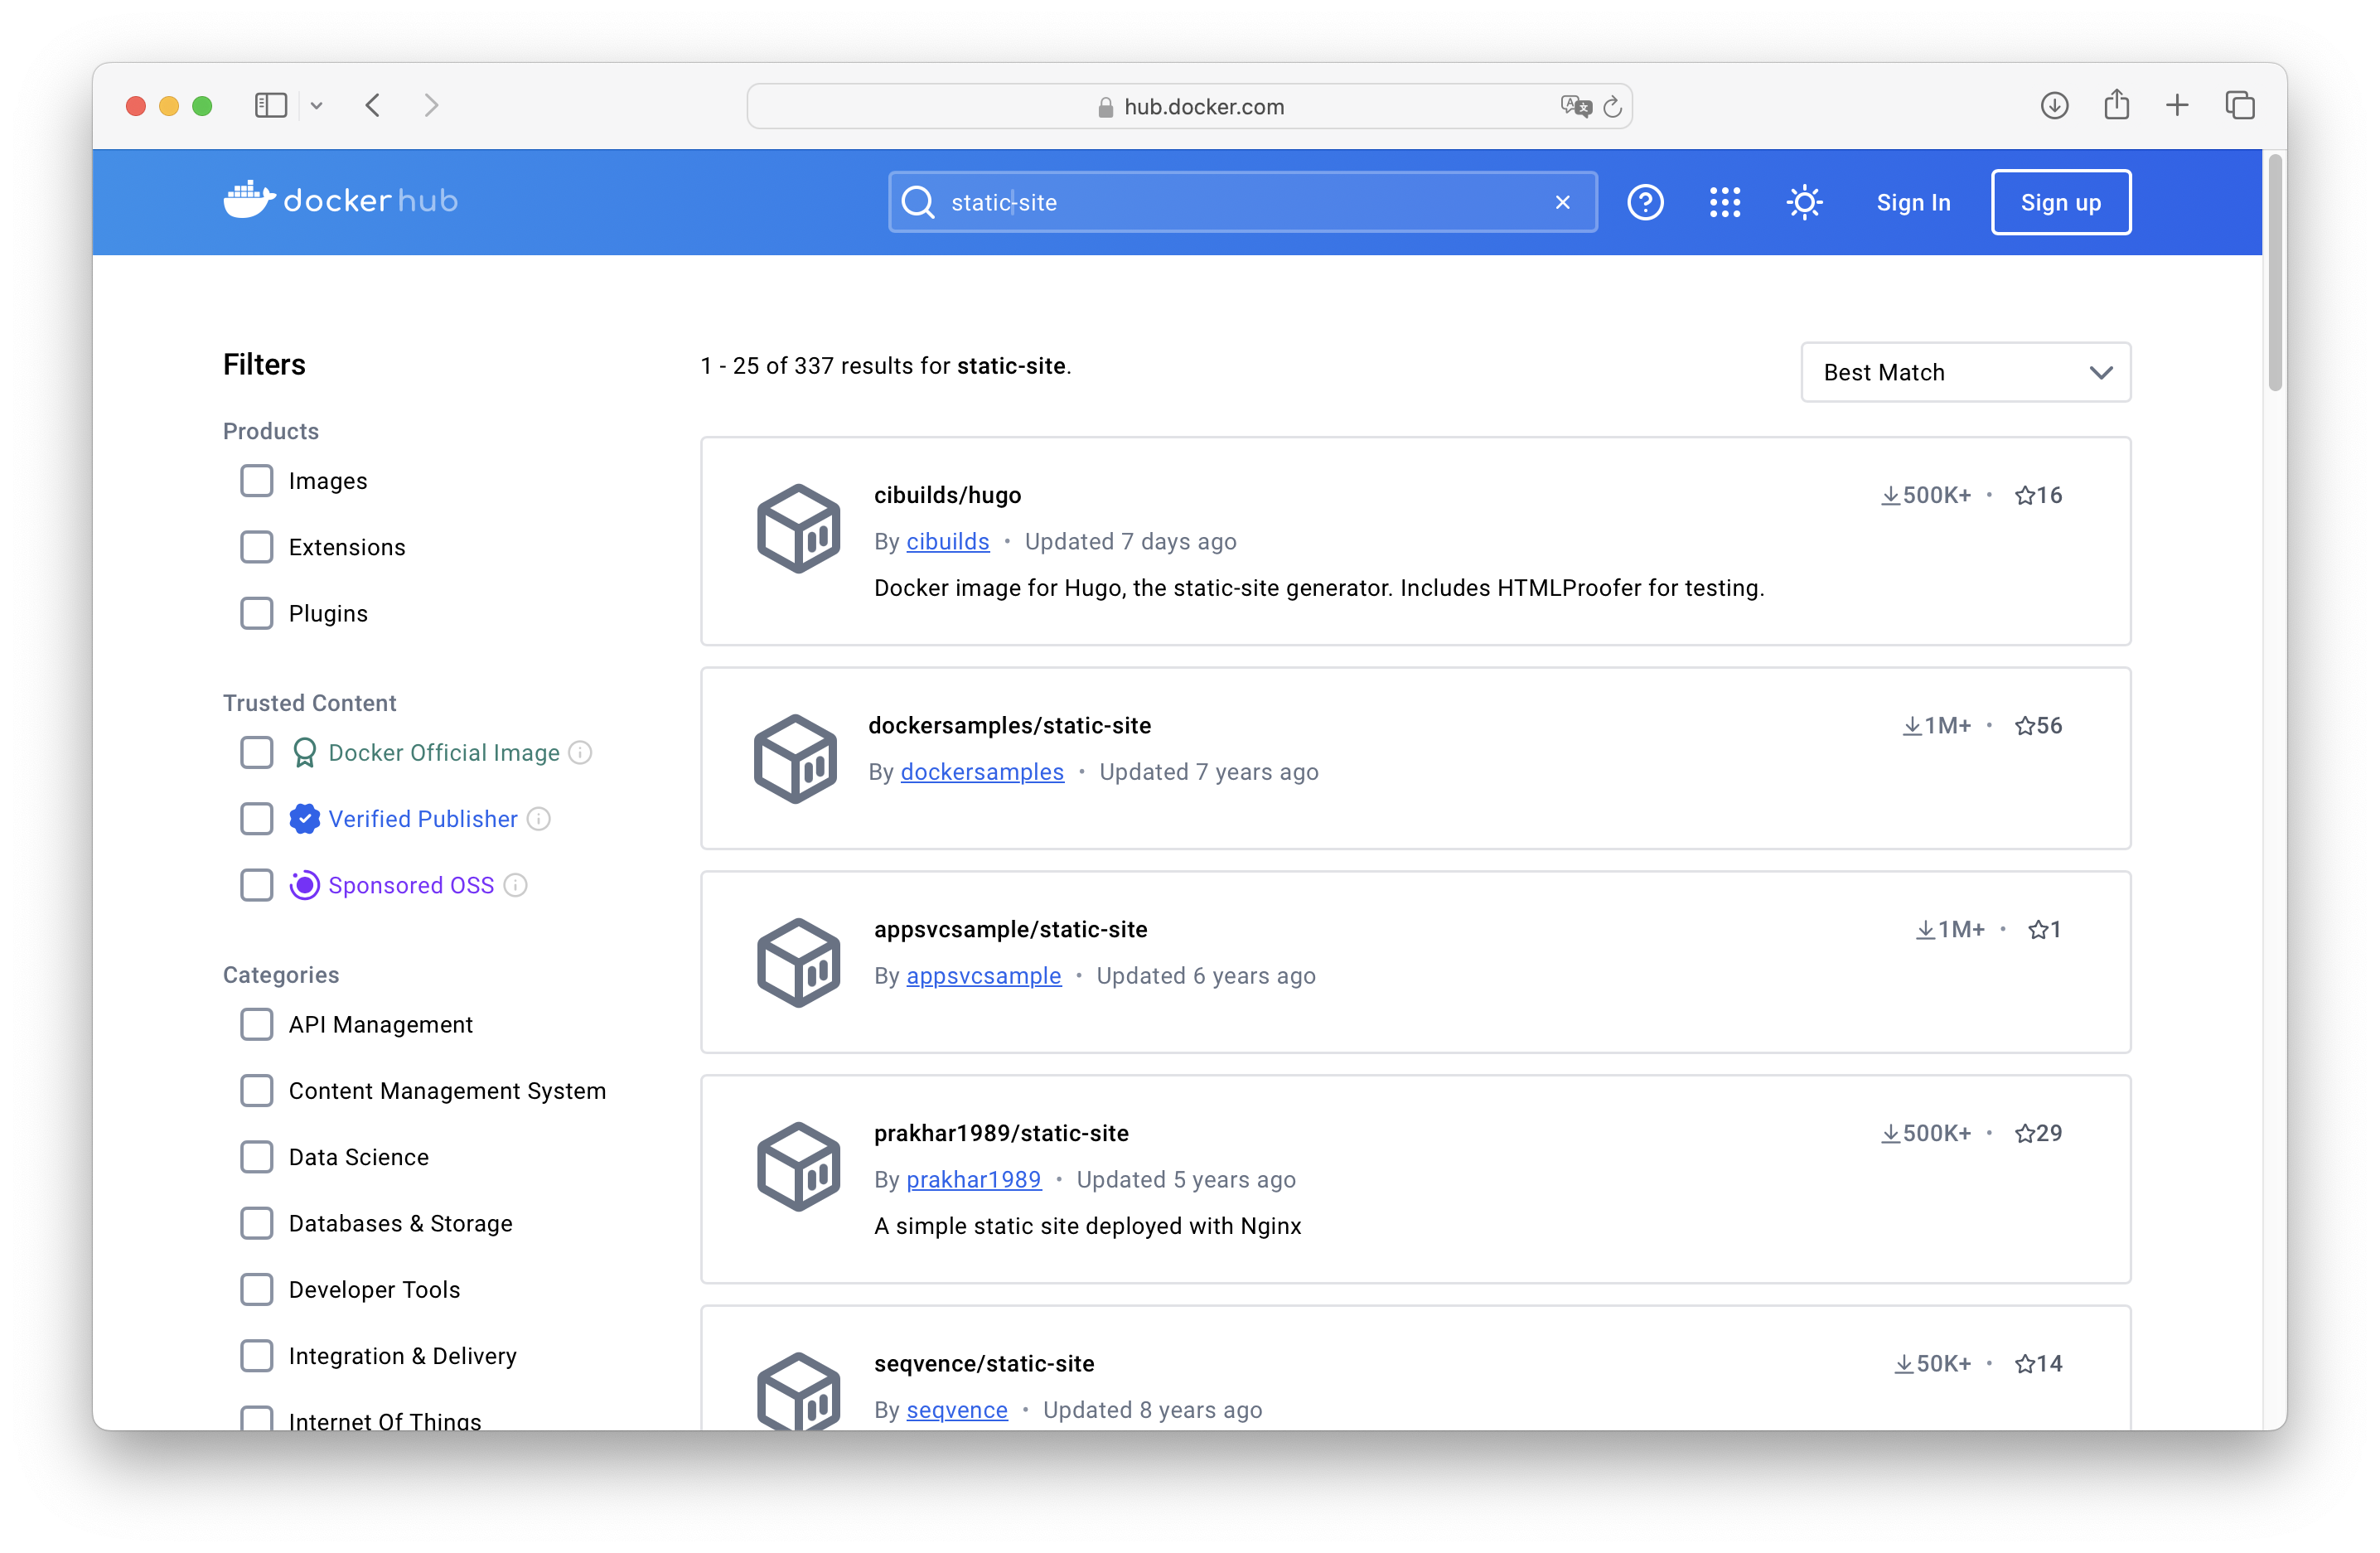
\includegraphics[width=.45\textwidth]{images/chapter4Images/ch4-1.png}
    \label{fig:nrGroup}
  }
  \hfill
  \subfloat[]{%
    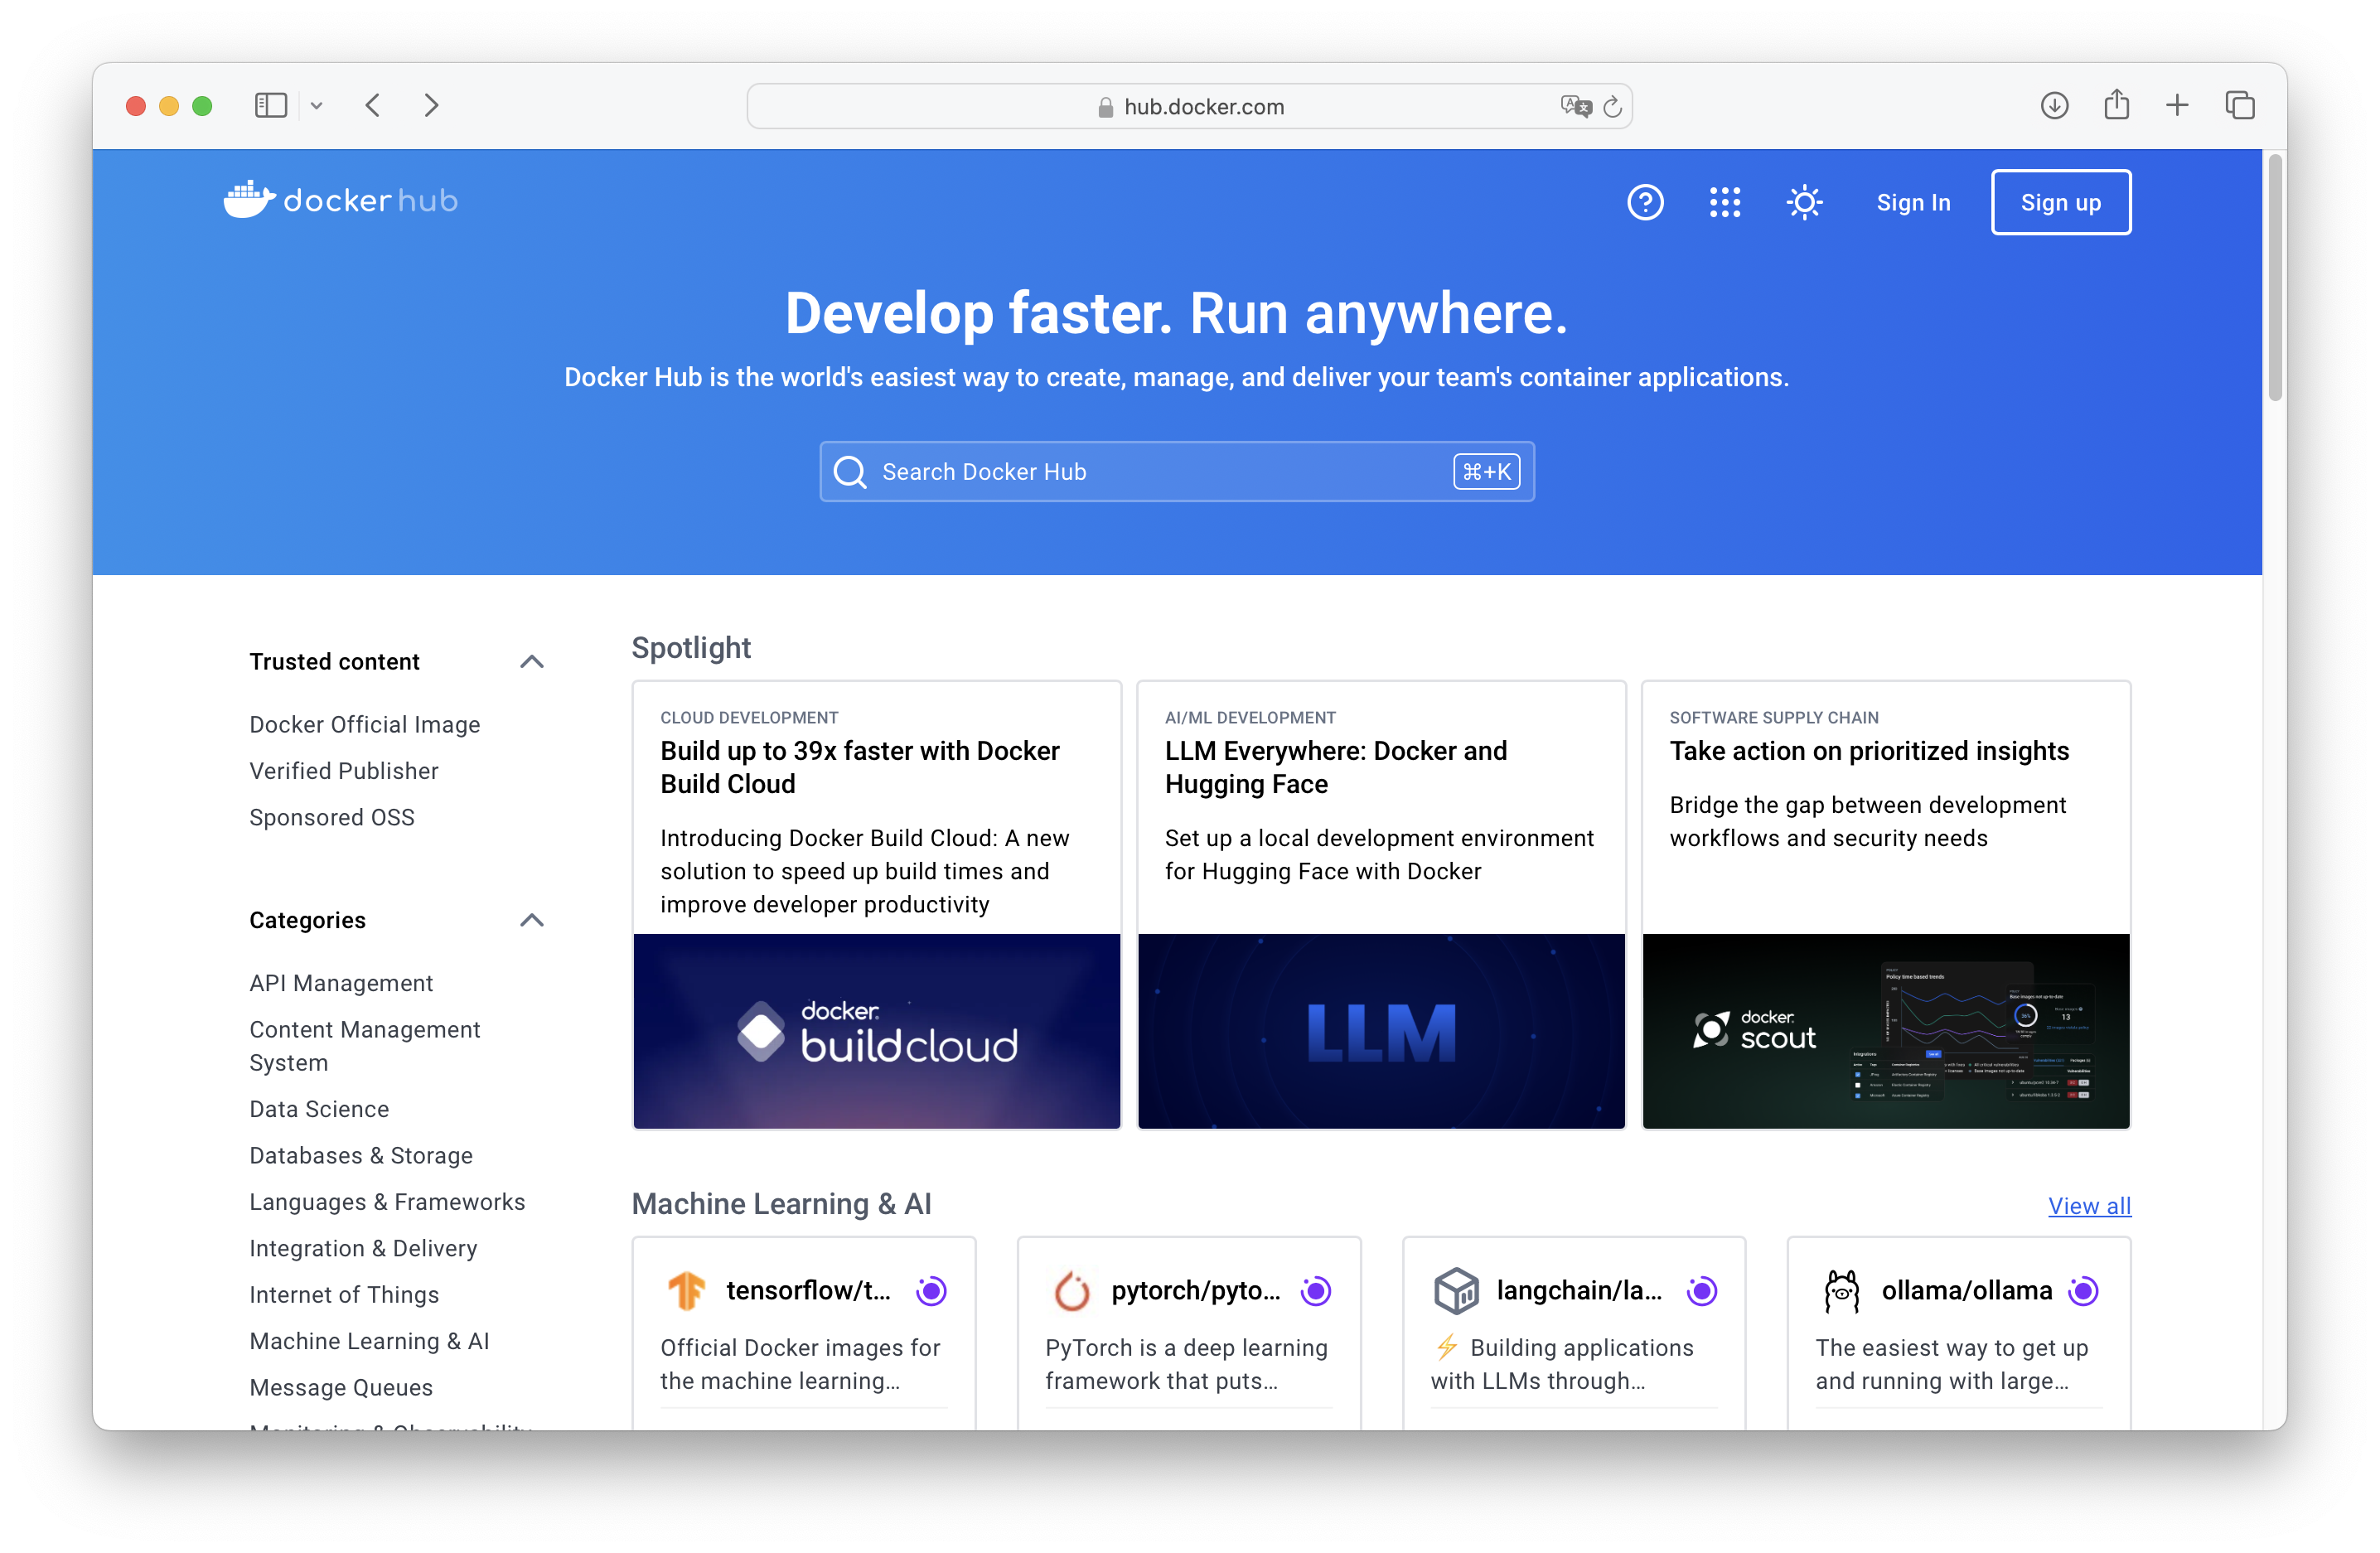
\includegraphics[width=.45\textwidth]{images/chapter4Images/ch4-2.png}
    \label{fig:zrGroup}
  }
  \caption{Docker Hub에서 static-site 이미지 가져오기}
  \label{fig:mainfig}
\end{figure*}

이 이미지는 Nginx 웹 서버를 실행하며, 이 서버는 컨테이너가 시작될 때 자동으로 시작됩니다. 이 이미지는 prakhar1989/static-site라는 이름으로 Docker Hub에 호스팅되었습니다. 이 이미지를 가져오고 실행하려면 다음 명령을 실행하세요.
\begin{lstlisting}[language=bash]
  $ sudo docker pull prakhar1989/static-site
  Using default tag: latest
  latest: Pulling from prakhar1989/static-site
  d4bce7fd68df: Pull complete 
  a3ed95caeb02: Pull complete 
  573113c4751a: Pull complete 
  31917632be33: Pull complete 
  77e66f18af1c: Pull complete 
  df3f108f3ade: Pull complete 
  d7a279eb19f5: Pull complete 
  e798589c05c5: Pull complete 
  78eeaf458ae0: Pull complete 
  Digest: sha256:bb6907c8db9ac4c6cadb25162a979e286575cd8b27727c08c7fbaf30988534db
  Status: Downloaded newer image for prakhar1989/static-site:latest
  docker.io/prakhar1989/static-site:latest
\end{lstlisting}

이미지가 로컬에 없으면 클라이언트가 먼저 레지스트리에서 이미지를 가져온 다음 이미지를 실행합니다. 모든 것이 잘 되면 터미널에 Nginx is running... 메시지가 표시됩니다. 이제 서버가 실행 중인데, 웹사이트를 어떻게 볼까요? 어떤 포트에서 실행되고 있나요? 더 중요한 것은 호스트 머신에서 컨테이너에 어떻게 액세스할까요? Ctrl+C를 눌러 컨테이너를 중지합니다.

이 경우 클라이언트가 포트를 노출하지 않으므로 포트를 게시하도록 docker run 명령을 다시 실행해야 합니다. 동시에 터미널이 실행 중인 컨테이너에 연결되지 않도록 해야 합니다. 이렇게 하면 터미널을 닫아도 컨테이너는 계속 실행됩니다. 이를 분리 모드라고 합니다.
\begin{lstlisting}[language=bash]
$ docker run -d -P --name static-site prakhar1989/static-site
e61d12292d69556eabe2a44c16cbd54486b2527e2ce4f95438e504afb7b02810
\end{lstlisting}

위 명령에서 -d는 터미널을 분리하고, -P는 모든 노출된 포트를 임의의 포트로 게시하며, --name은 컨테이너에 부여할 이름을 지정합니다. 이제 docker port [CONTAINER] 명령을 실행하여 포트를 확인할 수 있습니다.
\begin{lstlisting}[language=bash]
$ docker port static-site
80/tcp -> 0.0.0.0:32769
443/tcp -> 0.0.0.0:32768
\end{lstlisting}

브라우저에서 \url{http://localhost:32769}를 열 수 있습니다.
\begin{quote}
참고: docker-toolbox를 사용하는 경우 docker-machine ip default를 사용하여 IP를 가져와야 할 수 있습니다.
\end{quote}
클라이언트가 컨테이너로 연결을 전달할 포트를 지정할 수도 있습니다.
\begin{lstlisting}[language=bash]
$ docker run -p 8888:80 prakhar1989/static-site
Nginx is running...
\end{lstlisting}

\begin{figure}
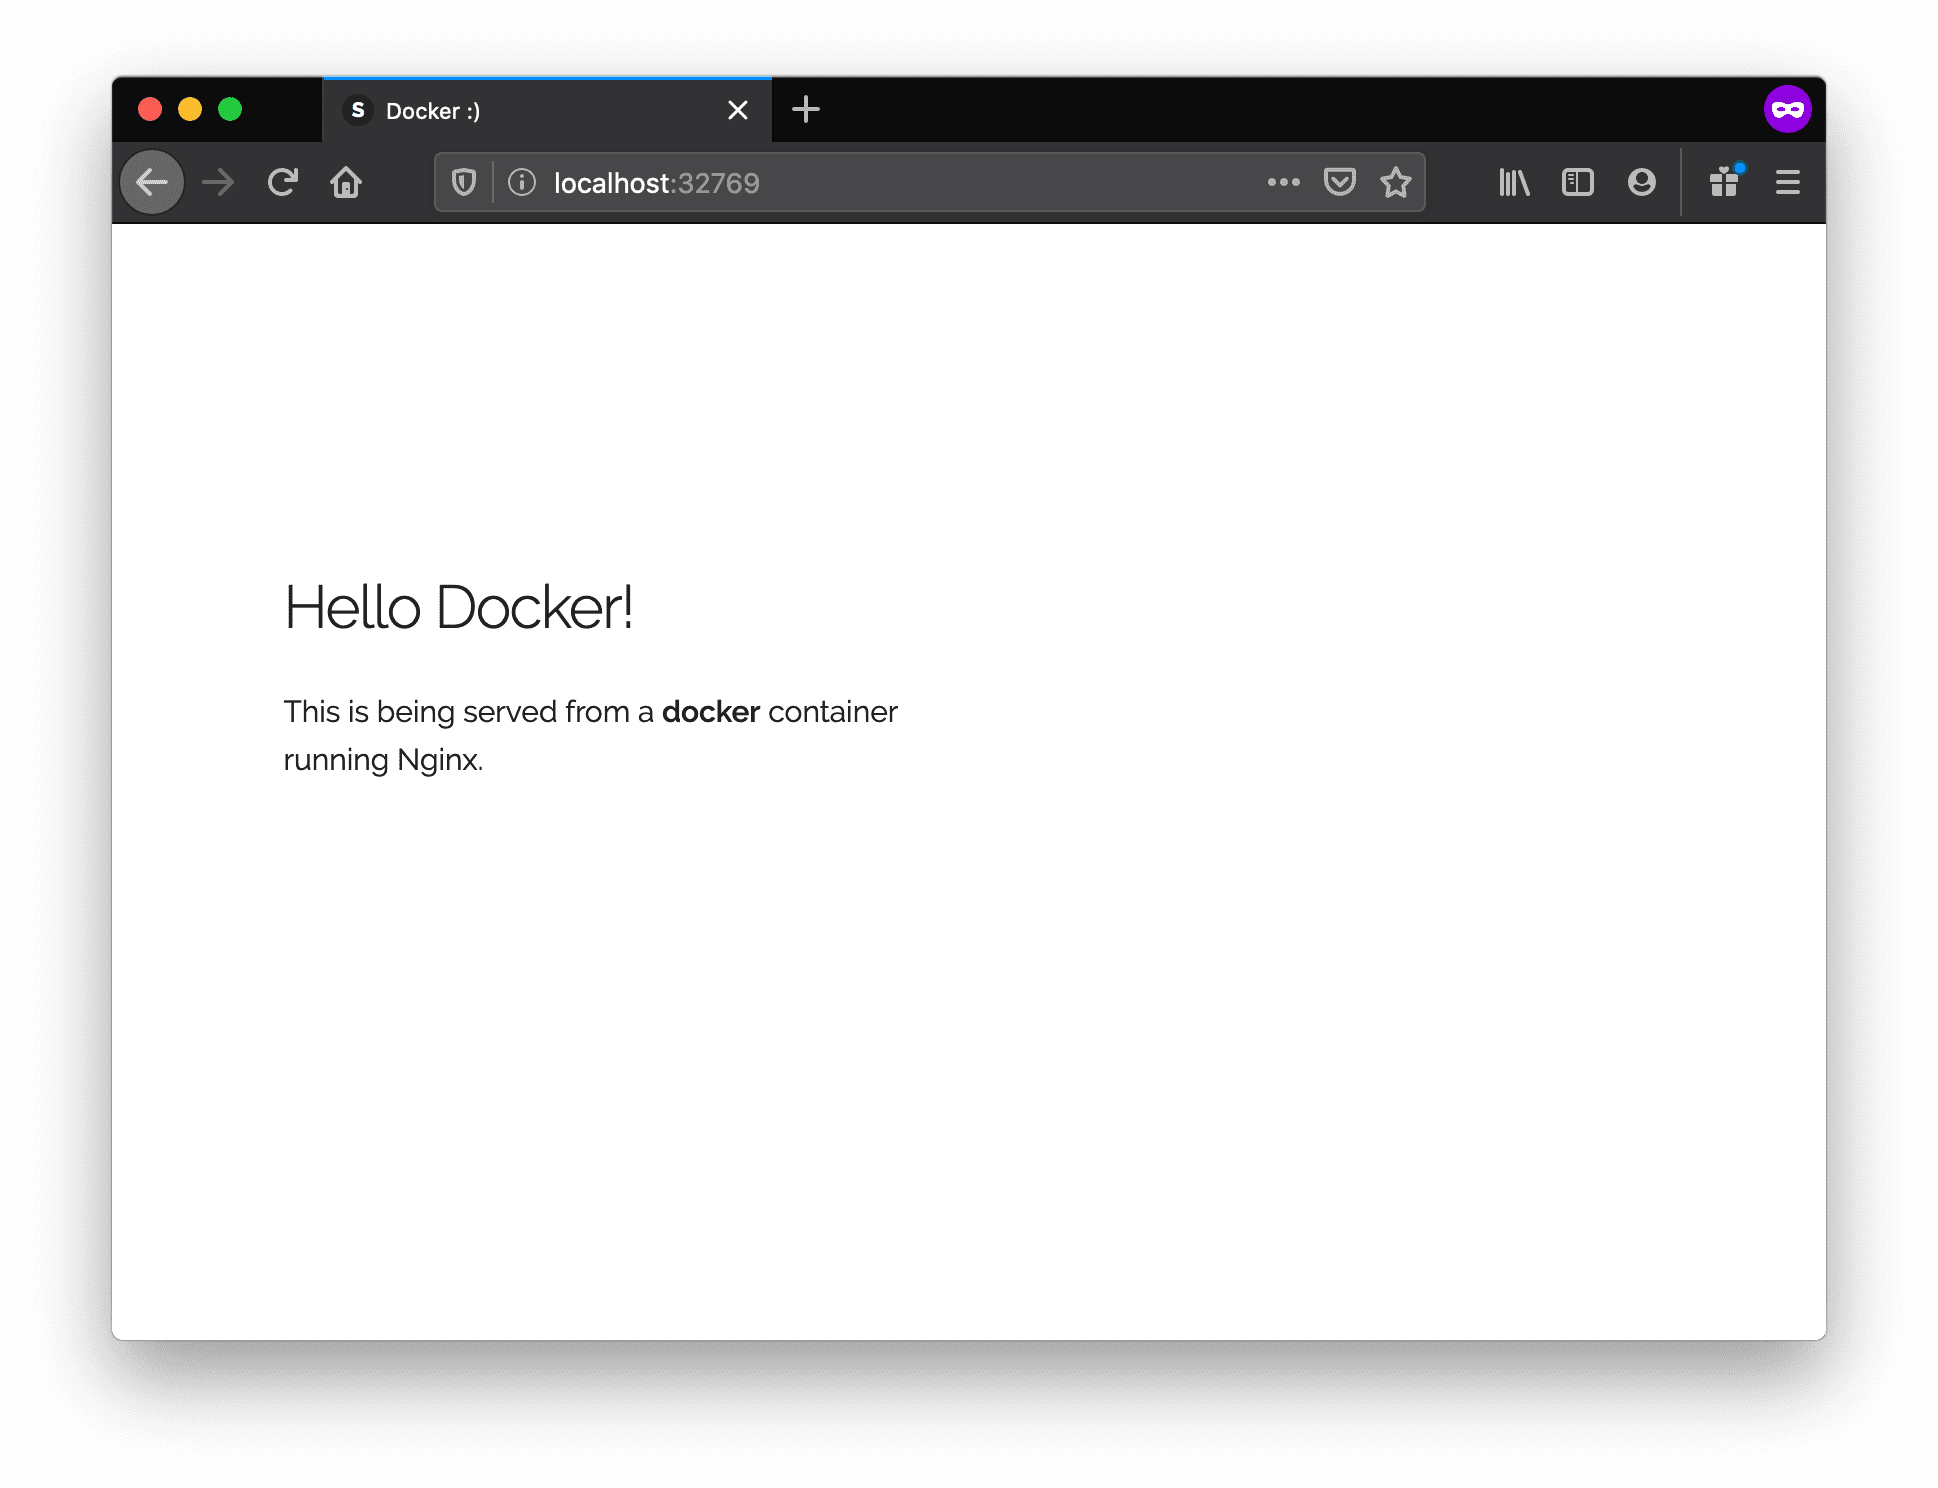
\includegraphics[width=\textwidth]{images/static.png}
\caption{Static Site}
\label{fig:static}
\end{figure}


분리된 컨테이너를 중지하려면 컨테이너 ID를 사용하여 docker stop 명령을 실행하세요. 이 경우 static-site라는 이름을 사용하여 컨테이너를 시작했습니다.
\begin{lstlisting}[language=bash]
$ docker stop static-site
static-site
\end{lstlisting}

매우 간단하죠. 실제 서버에 배포하려면 Docker를 설치하고 위 Docker 명령을 실행하면 됩니다. 이제 Docker 이미지를 사용하여 웹 서버를 실행하는 방법을 보았으므로, 자신만의 Docker 이미지를 생성하는 방법이 궁금할 것입니다. 다음 섹션에서 이를 탐구할 것입니다.

\section{Docker 이미지}
이미지를 이미 살펴보았지만, 이 섹션에서는 Docker 이미지가 무엇인지 더 자세히 살펴보고 직접 이미지를 만들어 보겠습니다! 마지막으로, 이 이미지를 사용하여 로컬에서 응용 프로그램을 실행하고 최종적으로 AWS에 배포하여 친구들과 공유할 것입니다! 흥미롭지 않나요? 그럼 시작해 봅시다.

Docker 이미지는 컨테이너의 기본입니다. 이전 예제에서는 Busybox 이미지를 레지스트리에서 가져와 Docker 클라이언트에 해당 이미지 기반의 컨테이너를 실행하도록 요청했습니다. 로컬에서 사용할 수 있는 이미지 목록을 보려면 docker images 명령을 사용하세요.
\begin{lstlisting}[language=bash]
$ docker images
REPOSITORY                      TAG                 IMAGE ID            CREATED             VIRTUAL SIZE
prakhar1989/catnip              latest              c7ffb5626a50        2 hours ago         697.9 MB
prakhar1989/static-site         latest              b270625a1631        21 hours ago        133.9 MB
python                          3-onbuild           cf4002b2c383        5 days ago          688.8 MB
martin/docker-cleanup-volumes   latest              b42990daaca2        7 weeks ago         22.14 MB
ubuntu                          latest              e9ae3c220b23        7 weeks ago         187.9 MB
busybox                         latest              c51f86c28340        9 weeks ago         1.109 MB
hello-world                     latest              0a6ba66e537a        11 weeks ago        960 B
\end{lstlisting}

위에는 레지스트리에서 가져온 이미지 목록과 직접 생성한 이미지 목록이 표시됩니다(곧 볼 수 있습니다). TAG는 이미지의 특정 스냅샷을 나타내며 IMAGE ID는 해당 이미지의 고유 식별자입니다.

간단히 말해, 이미지를 git 저장소와 유사하게 생각할 수 있습니다 - 이미지는 변경 사항을 커밋할 수 있으며 여러 버전을 가질 수 있습니다. 특정 버전 번호를 제공하지 않으면 클라이언트는 기본적으로 latest로 설정됩니다. 예를 들어, ubuntu 이미지의 특정 버전을 가져올 수 있습니다.
\begin{lstlisting}[language=bash]
$ docker pull ubuntu:18.04
\end{lstlisting}

새 Docker 이미지를 얻으려면 레지스트리(Docker Hub와 같은)에서 가져오거나 직접 생성할 수 있습니다. Docker Hub에는 수만 개의 이미지가 있습니다. 커맨드 라인을 사용하여 docker search로 이미지를 검색할 수도 있습니다.

이미지와 관련하여 주의해야 할 중요한 차이점은 기본 이미지와 자식 이미지의 차이입니다.
\begin{itemize}
    \item \textbf{기본 이미지}는 부모 이미지가 없는 이미지로, 보통 ubuntu, busybox 또는 debian과 같은 운영 체제가 있는 이미지입니다.
    \item \textbf{자식 이미지}는 기본 이미지를 기반으로 추가 기능을 제공하는 이미지입니다.
\end{itemize}

그다음으로 공식 이미지와 사용자 이미지가 있으며, 이 둘 다 기본 이미지와 자식 이미지가 될 수 있습니다.
\begin{itemize}
    \item \textbf{공식 이미지}는 Docker 팀에서 공식적으로 유지 관리하고 지원하는 이미지입니다. 이러한 이미지는 일반적으로 한 단어로 이루어져 있습니다. 위의 이미지 목록에서 python, ubuntu, busybox 및 hello-world 이미지는 공식 이미지입니다.
    \item \textbf{사용자 이미지}는 사용자(여러분과 같은)가 생성하고 공유한 이미지입니다. 기본 이미지를 기반으로 추가 기능을 제공합니다. 일반적으로 user/image-name 형식으로 작성됩니다.
\end{itemize}

\section{우리의 첫 번째 이미지}
이미지에 대한 이해가 깊어졌으니 이제 직접 이미지를 만들어 봅시다. 이 섹션의 목표는 간단한 Flask 응용 프로그램을 샌드박싱하는 이미지를 만드는 것입니다. 이 튜토리얼을 위해 귀여운 작은 Flask 앱을 이미 만들어 두었으며, 이 앱은 로드될 때마다 랜덤한 고양이 gif를 표시합니다. 고양이를 좋아하지 않는 사람이 누가 있겠습니까? 아직 하지 않았다면 다음 명령을 사용하여 로컬 저장소를 클론하세요 -
\begin{lstlisting}[language=bash]
$ git clone https://github.com/prakhar1989/docker-curriculum.git
$ cd docker-curriculum/flask-app
\end{lstlisting}

\begin{quote}
이 작업은 docker 명령을 실행하는 머신에서 클론해야 하며, Docker 컨테이너 내부에서는 클론하지 마세요.
\end{quote}

다음 단계는 이 웹 앱을 포함하는 이미지를 만드는 것입니다. 위에서 언급한 것처럼 모든 사용자 이미지는 기본 이미지를 기반으로 합니다. 우리의 응용 프로그램이 Python으로 작성되었기 때문에 사용할 기본 이미지는 Python 3가 될 것입니다.

\section{Dockerfile}
Dockerfile은 이미지 생성 시 Docker 클라이언트가 호출하는 명령 목록이 포함된 간단한 텍스트 파일입니다. 이미지 생성 프로세스를 자동화하는 간단한 방법입니다. 가장 좋은 점은 Dockerfile에서 작성하는 명령이 리눅스 명령과 거의 동일하다는 것입니다. 따라서 Dockerfile을 작성하기 위해 새로운 문법을 배울 필요가 없습니다.

응용 프로그램 디렉토리에 Dockerfile이 포함되어 있지만 처음으로 이 작업을 수행하므로 처음부터 새로 만들겠습니다. 좋아하는 텍스트 편집기에서 빈 파일을 생성하고 flask 앱과 같은 폴더에 Dockerfile이라는 이름으로 저장하세요.

기본 이미지를 지정하는 것부터 시작합니다. FROM 키워드를 사용하세요 -
\begin{lstlisting}[language=dockerfile]
FROM python:3.8
\end{lstlisting}

다음 단계는 파일을 복사하고 종속성을 설치하는 명령을 작성하는 것입니다. 먼저 작업 디렉토리를 설정한 다음 응용 프로그램의 모든 파일을 복사합니다.
\begin{lstlisting}[language=dockerfile]
# Set the working directory for the application
WORKDIR /usr/src/app
# Copy all files to the container
COPY . .
\end{lstlisting}

이제 파일을 복사했으므로 종속성을 설치할 수 있습니다.
\begin{lstlisting}[language=dockerfile]
# Install dependencies
RUN pip install --no-cache-dir -r requirements.txt
\end{lstlisting}

다음으로 노출해야 할 포트 번호를 지정해야 합니다. Flask 앱이 5000 포트에서 실행되므로 이를 표시하겠습니다.
\begin{lstlisting}[language=dockerfile]
EXPOSE 5000
\end{lstlisting}

마지막 단계는 응용 프로그램을 실행하는 명령을 작성하는 것입니다. 이는 단순히 python ./app.py입니다. 이를 위해 CMD 명령을 사용합니다 -
\begin{lstlisting}[language=dockerfile]
CMD [ "python", "./app.py" ]
\end{lstlisting}

CMD의 주요 목적은 컨테이너 시작 시 실행할 명령을 지정하는 것입니다. 이렇게 하면 Dockerfile이 준비됩니다. 다음과 같이 보일 것입니다 -
\begin{lstlisting}[language=dockerfile]
FROM python:3.8

# Set the working directory for the application
WORKDIR /usr/src/app
# Copy all files to the container
COPY . .
# Install dependencies
RUN pip install --no-cache-dir -r requirements.txt
# Define the port number the container should expose
EXPOSE 5000
# Run the command
CMD ["python", "./app.py"]
\end{lstlisting}

이제 Dockerfile이 준비되었으므로 이미지를 빌드할 수 있습니다. docker build 명령은 Dockerfile에서 Docker 이미지를 생성하는 작업을 수행합니다.

아래 섹션에서는 동일한 명령을 실행한 출력을 보여줍니다. 명령을 직접 실행하기 전에(점을 잊지 마세요) 제 사용자 이름을 여러분의 사용자 이름으로 바꾸세요. 이 사용자 이름은 Docker Hub에 등록할 때 생성한 사용자 이름과 동일해야 합니다. 아직 계정을 생성하지 않았다면, 지금 바로 생성해 주세요. docker build 명령은 매우 간단합니다 - 선택적으로 -t와 위치를 사용하여 태그 이름과 Dockerfile이 포함된 디렉토리를 지정할 수 있습니다.
\begin{lstlisting}[language=bash]
$ docker build -t yourusername/catnip .
Sending build context to Docker daemon 8.704 kB
Step 1 : FROM python:3.8
# Executing 3 build triggers...
Step 1 : COPY requirements.txt /usr/src/app/
 ---> Using cache
Step 1 : RUN pip install --no-cache-dir -r requirements.txt
 ---> Using cache
Step 1 : COPY . /usr/src/app
 ---> 1d61f639ef9e
Removing intermediate container 4de6ddf5528c
Step 2 : EXPOSE 5000
 ---> Running in 12cfcf6d67ee
 ---> f423c2f179d1
Removing intermediate container 12cfcf6d67ee
Step 3 : CMD python ./app.py
 ---> Running in f01401a5ace9
 ---> 13e87ed1fbc2
Removing intermediate container f01401a5ace9
Successfully built 13e87ed1fbc2
\end{lstlisting}

python:3.8 이미지를 가지고 있지 않다면, 클라이언트가 먼저 이미지를 가져오고 나서 여러분의 이미지를 생성할 것입니다. 따라서 명령을 실행한 출력은 저와 다를 것입니다. 모든 것이 잘 되었다면, 이미지는 준비되었을 것입니다! docker images를 실행하여 이미지가 표시되는지 확인하세요.

이 섹션의 마지막 단계는 이미지를 실행하고 실제로 작동하는지 확인하는 것입니다(제 사용자 이름을 여러분의 사용자 이름으로 바꾸세요).
\begin{lstlisting}[language=bash]
$ docker run -p 8888:5000 yourusername/catnip
 * Running on http://0.0.0.0:5000/ (Press CTRL+C to quit)
\end{lstlisting}

방금 실행한 명령은 컨테이너 내부의 서버에 5000 포트를 사용하고 이를 외부적으로 8888 포트에서 노출했습니다. 8888 포트를 사용하는 URL로 이동하면 앱이 활성화된 것을 볼 수 있습니다.

\begin{figure}
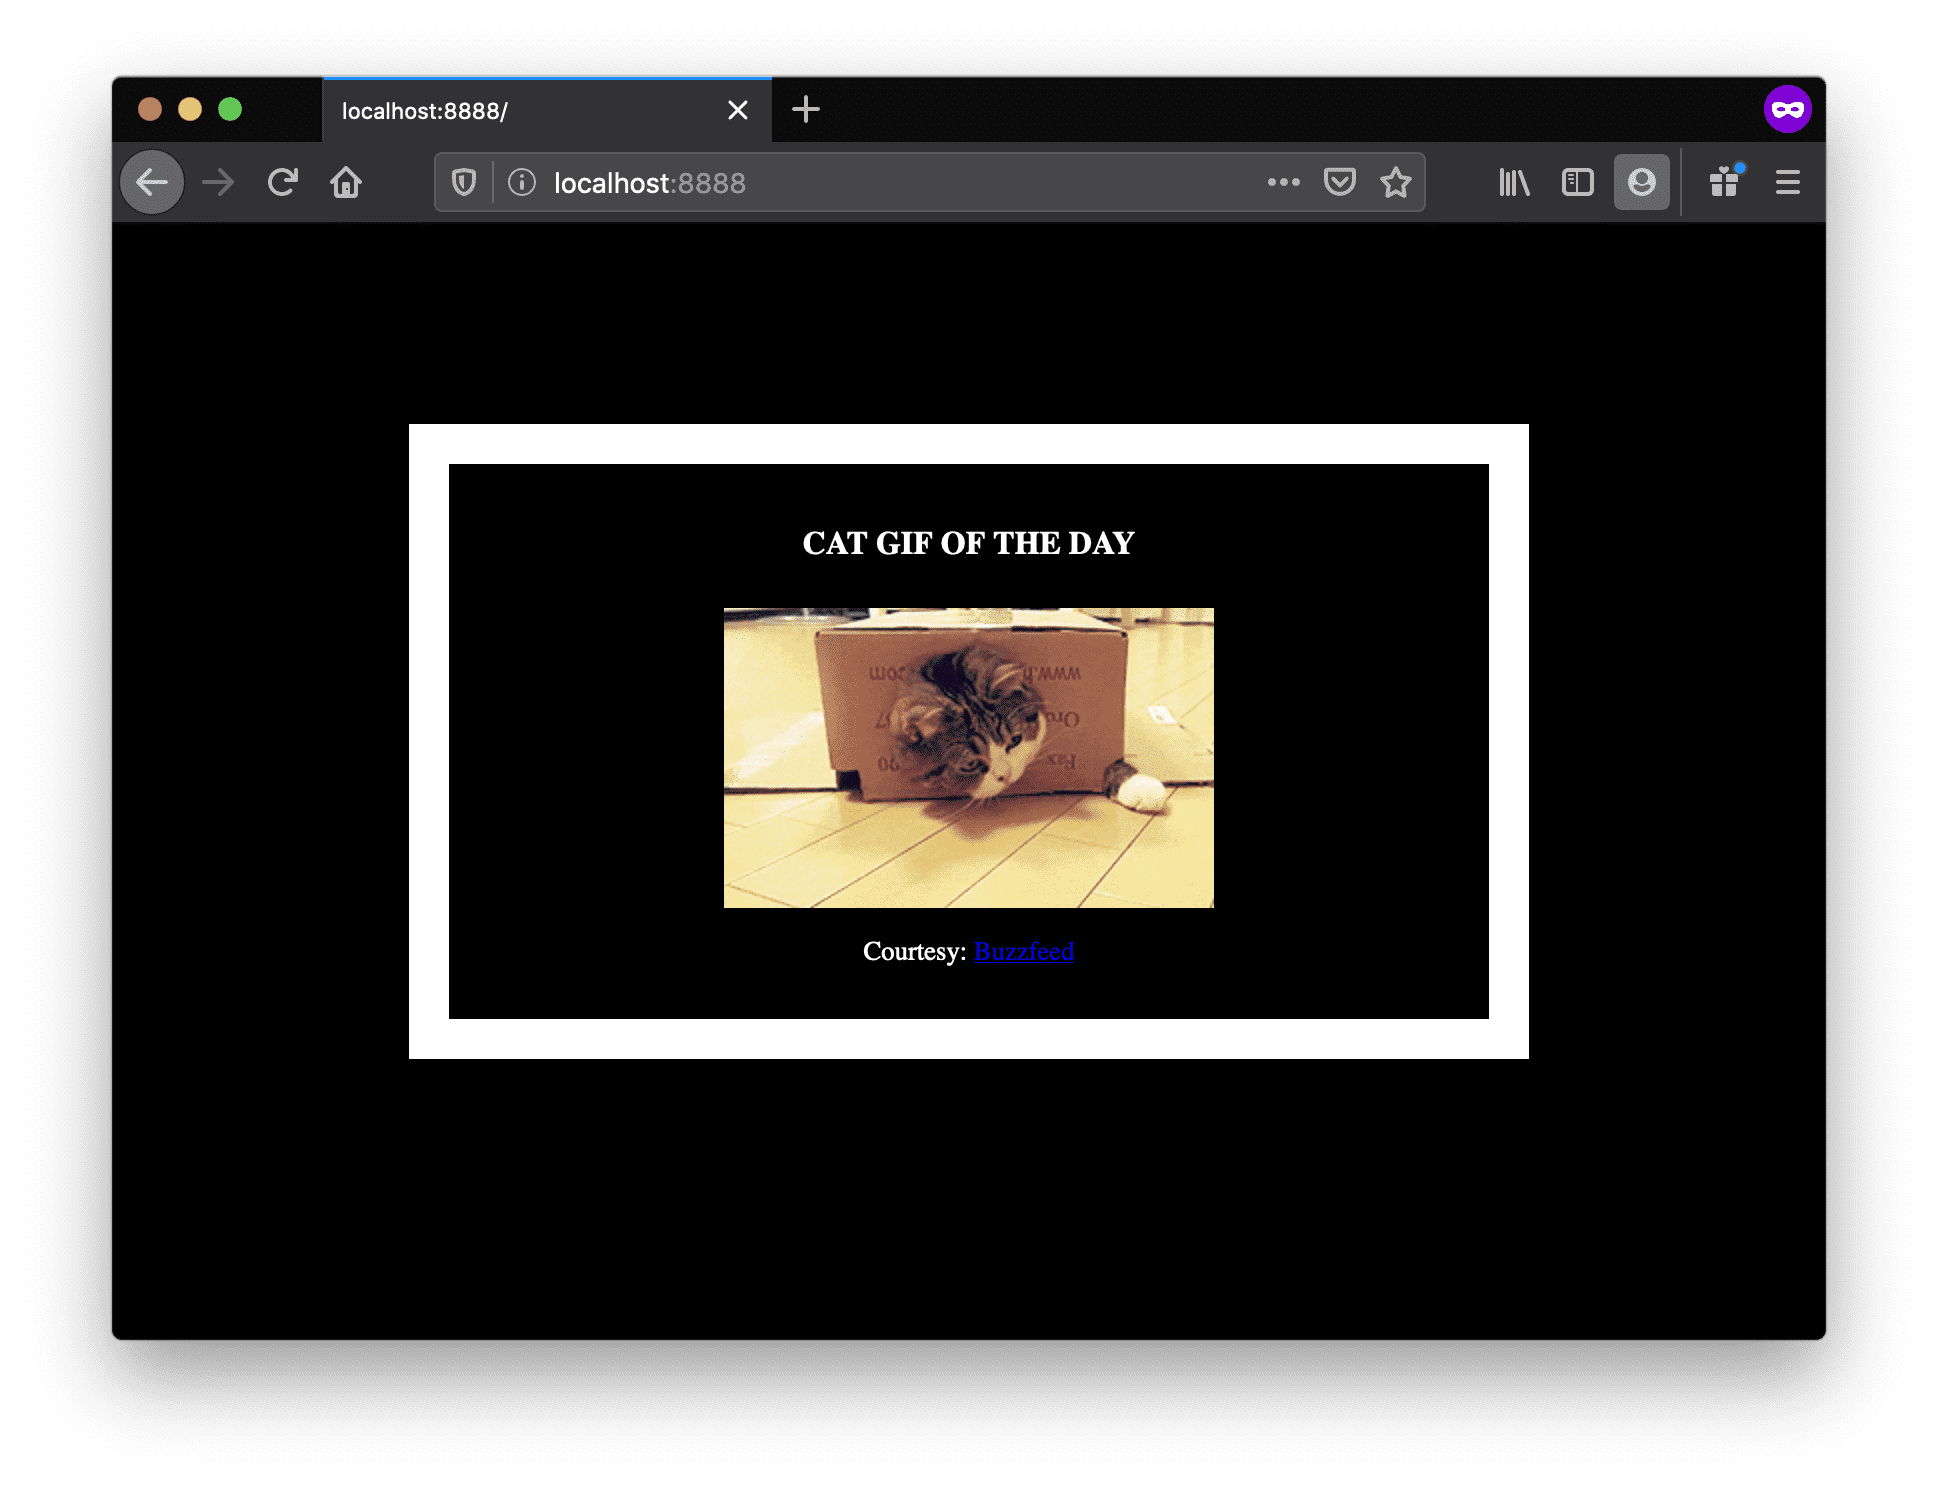
\includegraphics[width=\textwidth]{images/catgif.png}
\caption{Cat GIF Website}
\end{figure}

축하합니다! 첫 번째 Docker 이미지를 성공적으로 생성했습니다.

\section{AWS에서 Docker}
응용 프로그램을 친구와 공유할 수 없다면 무슨 소용이 있을까요? 이 섹션에서는 응용 프로그램을 클라우드에 배포하여 친구와 공유할 수 있도록 하는 방법을 살펴보겠습니다! 우리는 AWS Elastic Beanstalk을 사용하여 몇 번의 클릭만으로 응용 프로그램을 실행할 것입니다. 또한 Beanstalk을 사용하여 응용 프로그램을 확장하고 관리하는 것이 얼마나 쉬운지 볼 것입니다!

\subsection{Docker push}
AWS에 앱을 배포하기 전에 해야 할 첫 번째 일은 AWS에서 접근할 수 있는 레지스트리에 이미지를 게시하는 것입니다. 사용할 수 있는 Docker 레지스트리에는 여러 가지가 있습니다(자신만의 레지스트리를 호스팅할 수도 있습니다). 지금은 Docker Hub를 사용하여 이미지를 게시하겠습니다.

이미지를 처음으로 푸시하는 경우 클라이언트가 로그인하라는 메시지를 표시할 것입니다. Docker Hub에 로그인할 때 사용한 것과 동일한 자격 증명을 제공하세요.
\begin{lstlisting}[language=bash]
$ docker login
Login in with your Docker ID to push and pull images from Docker Hub. If you do not have a Docker ID, head over to https://hub.docker.com to create one.
Username: yourusername
Password:
WARNING! Your password will be stored unencrypted in /Users/yourusername/.docker/config.json
Configure a credential helper to remove this warning. See https://docs.docker.com/engine/reference/commandline/login/credential-store

Login Succeeded
\end{lstlisting}

게시하려면 위 이미지 태그의 이름을 여러분의 이름으로 바꾸는 것을 기억하면서 아래 명령을 입력하세요. 클라이언트가 어디에 게시할지 알 수 있도록 $yourusername/image_name$ 형식을 유지하는 것이 중요합니다.
\begin{lstlisting}[language=bash]
$ docker push yourusername/catnip
\end{lstlisting}

이 작업이 완료되면 Docker Hub에서 여러분의 이미지를 볼 수 있습니다. 예를 들어, 여기는 제 이미지의 웹 페이지입니다.
\begin{quote}
참고: 앞으로 나아가기 전에 명확히 하고 싶은 것은, AWS에 배포하기 위해 이미지를 공개 레지스트리(또는 어떤 레지스트리)에 호스팅하는 것이 필수적이지 않다는 것입니다. 다음 백만 달러 스타트업을 위한 코드를 작성하는 경우 이 단계를 건너뛸 수 있습니다. 이미지를 공개적으로 푸시하는 이유는 중간 구성 단계를 건너뛰어 배포를 매우 간단하게 만들기 때문입니다.
\end{quote}
이제 여러분의 이미지가 온라인에 있으므로 Docker가 설치된 누구나 단일 명령으로 여러분의 앱을 사용할 수 있습니다.
\begin{lstlisting}[language=bash]
$ docker run -p 8888:5000 yourusername/catnip
\end{lstlisting}

로컬 개발 환경 설정 / 응용 프로그램 구성을 공유하는 데 어려움을 겪은 적이 있다면, 이것이 얼마나 멋진 것인지 알 것입니다. 이것이 Docker가 멋진 이유입니다!

\subsection{Beanstalk}
AWS Elastic Beanstalk (EB)은 AWS에서 제공하는 PaaS (Platform as a Service)입니다. Heroku, Google App Engine 등을 사용해 본 적이 있다면 익숙할 것입니다. 개발자로서 여러분은 EB에게 앱을 어떻게 실행할지 알려주기만 하면 나머지는 EB가 처리합니다 - 확장, 모니터링 및 업데이트를 포함하여. 2014년 4월에 EB는 단일 컨테이너 Docker 배포를 지원하기 시작했으며, 이를 사용하여 앱을 배포할 것입니다. EB는 매우 직관적인 CLI를 가지고 있지만, 일부 설정이 필요하므로 간단하게 유지하기 위해 웹 UI를 사용하여 응용 프로그램을 시작하겠습니다.

따라하려면 기능하는 AWS 계정이 필요합니다. 아직 계정이 없으신 분은 지금 바로 만들어 주세요 - 신용 카드 정보를 입력해야 합니다. 걱정하지 마세요, 무료입니다. 이 튜토리얼에서 하는 모든 작업도 무료입니다! 시작해 봅시다.

단계는 다음과 같습니다:
\begin{itemize}
    \item AWS 콘솔에 로그인하세요.
    \item Elastic Beanstalk을 클릭하세요. 왼쪽 상단의 컴퓨팅 섹션에 있을 것입니다. 또는 Elastic Beanstalk 콘솔에 액세스할 수 있습니다.
\end{itemize}

\begin{figure}
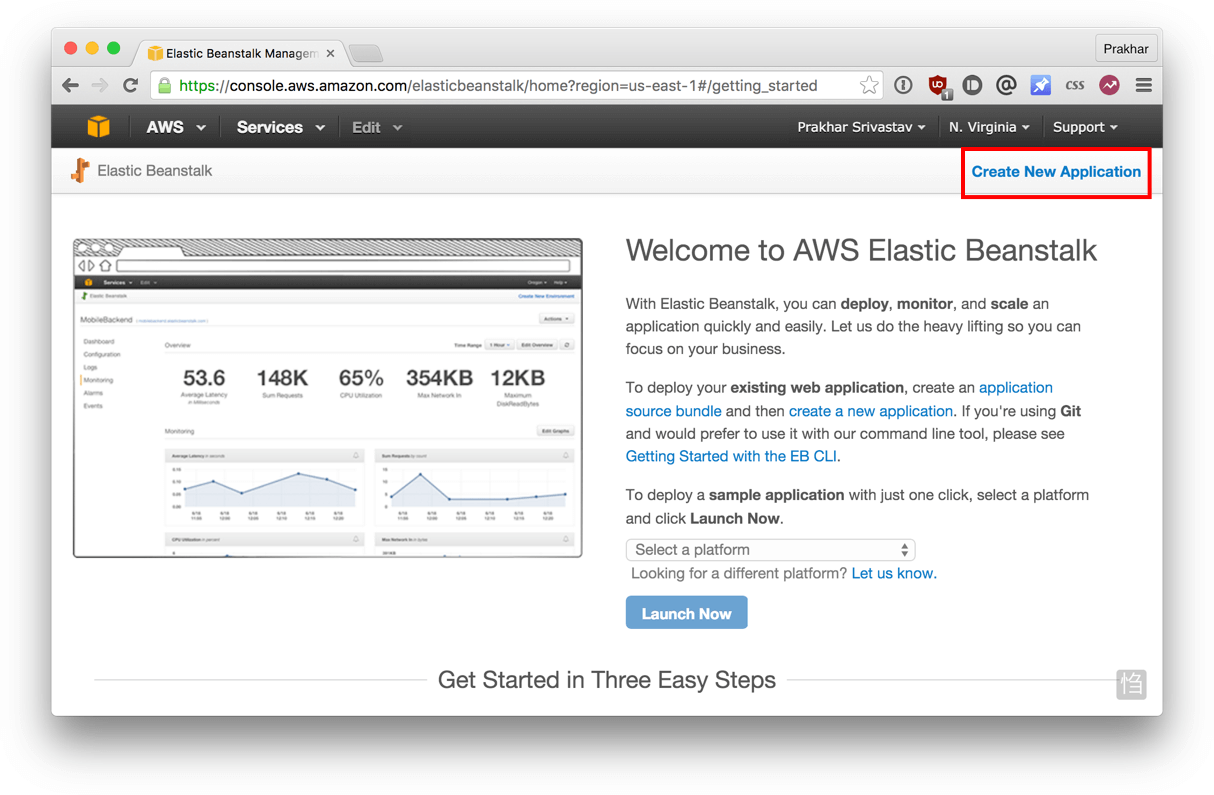
\includegraphics[width=\textwidth]{images/eb-start.png}
\caption{Elastic Beanstalk Start}
\label{fig:eb-start}
\end{figure}


\begin{itemize}
    \item 오른쪽 상단의 "새 응용 프로그램 생성"을 클릭하세요.
    \item 기억할 수 있는(그러나 고유한) 이름을 입력하고(선택 사항) 설명을 입력하세요.
    \item 새 환경 화면에서 새 환경을 만들고 웹 서버 환경을 선택하세요.
    \item 도메인을 선택하여 환경 정보를 입력하세요. 이 URL은 친구와 공유할 URL이므로 기억하기 쉬운 것으로 선택하세요.
    \item 기본 구성 섹션에서 미리 정의된 플랫폼에서 Docker를 선택하세요.
\end{itemize}

\begin{figure}
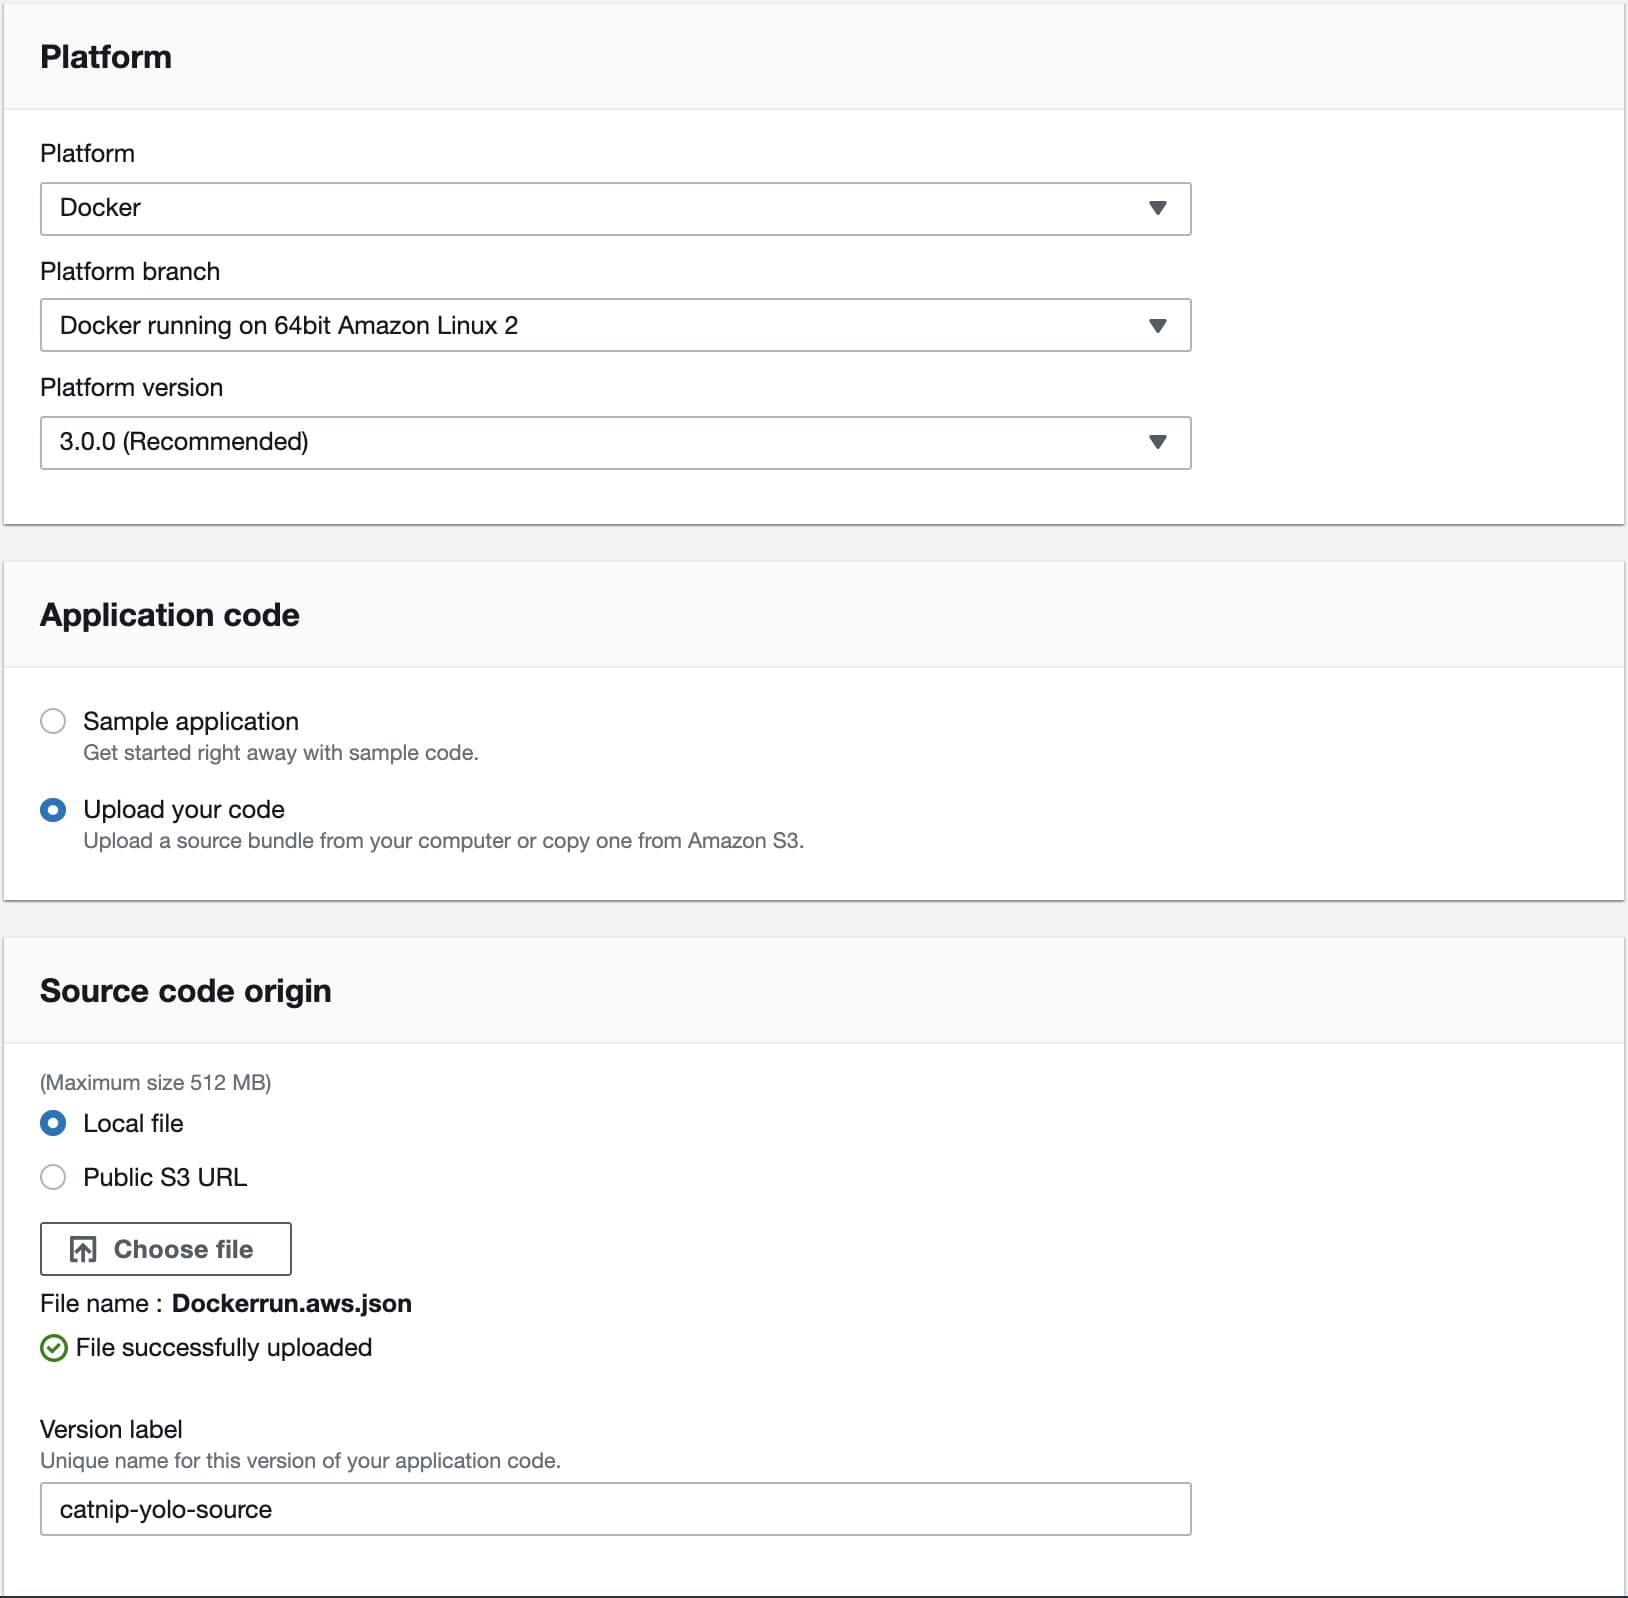
\includegraphics[width=\textwidth]{images/eb-docker.jpeg}
\caption{Elastic Beanstalk Environment Type}
\end{figure}


\begin{itemize}
    \item 이제 응용 프로그램 코드를 업로드해야 합니다. 그러나 응용 프로그램이 Docker 컨테이너로 패키징되었기 때문에 EB에게 컨테이너에 대해 알려주기만 하면 됩니다. flask-app 폴더에 있는 Dockerrun.aws.json 파일을 열고 이미지의 이름을 자신의 이미지 이름으로 편집하세요. 파일 내용을 곧 설명하겠습니다. 완료되면 "코드 업로드" 라디오 버튼을 선택하고 이 파일을 선택한 다음 "업로드"를 클릭하세요.
    \item "환경 생성"을 클릭하세요. 최종 화면에 환경이 설정 중이라는 스피너가 표시됩니다. 처음 설정에는 약 5분이 걸립니다.
\end{itemize}
기다리는 동안 Dockerrun.aws.json 파일에 무엇이 들어 있는지 간략히 살펴보겠습니다. 이 파일은 AWS 전용 파일로, EB에게 응용 프로그램 및 Docker 구성에 대한 세부 정보를 제공합니다.
\begin{lstlisting}[language=dockerfile]
{
  "AWSEBDockerrunVersion": "1",
  "Image": {
    "Name": "prakhar1989/catnip",
    "Update": "true"
  },
  "Ports": [
    {
      "ContainerPort": 5000,
      "HostPort": 8000
    }
  ],
  "Logging": "/var/log/nginx"
}
\end{lstlisting}

파일은 매우 간단하지만, 공식 문서를 참조하여 더 많은 정보를 얻을 수 있습니다. EB에게 사용할 이미지의 이름과 컨테이너가 열어야 할 포트를 제공합니다.

이제 인스턴스가 준비되었을 것입니다. EB 페이지로 이동하면 앱이 활성화되고 있는지 표시하는 녹색 체크 표시를 볼 수 있습니다.
\begin{figure}
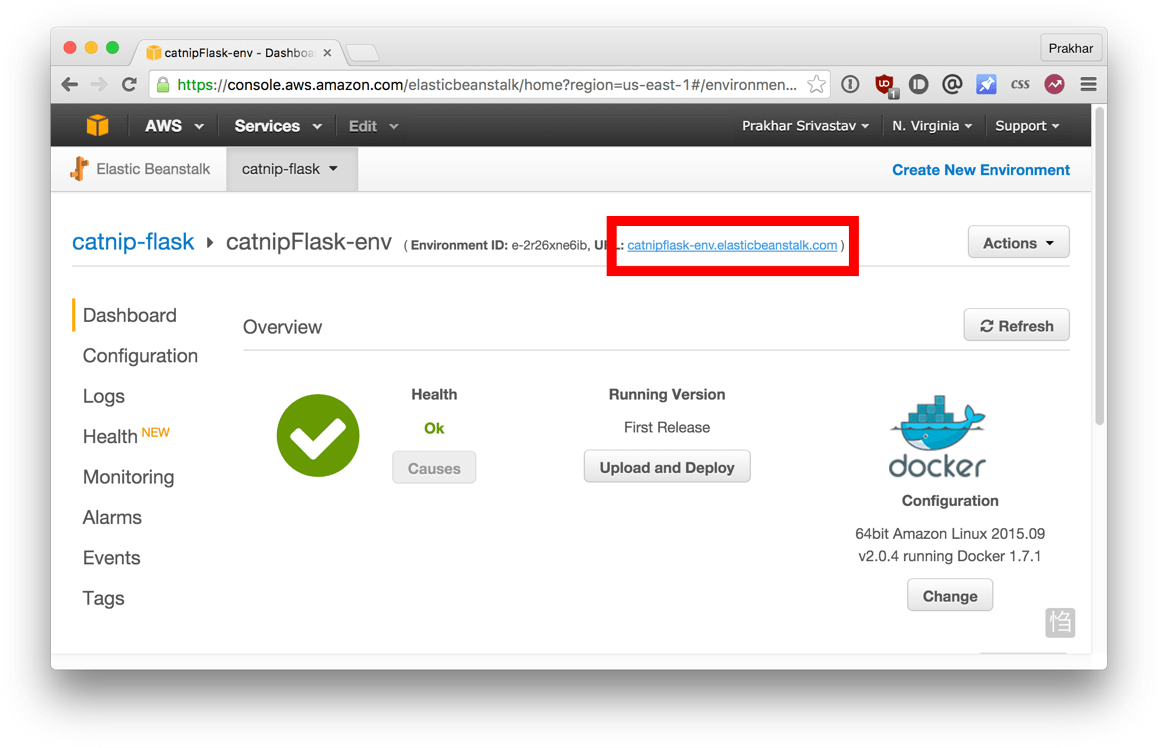
\includegraphics[width=\textwidth]{images/eb-deploy.png}
\caption{EB Deploy}
\end{figure}



브라우저에서 URL을 열고 응용 프로그램이 실행되는 것을 확인하세요. 이 링크를 친구와 가족에게 이메일 / IM / 스냅챗으로 보내서 고양이 gif를 즐길 수 있도록 하세요.

\subsection{정리}
응용 프로그램의 영광을 즐긴 후에는 추가 리소스에 대한 비용이 청구되지 않도록 환경을 종료하는 것을 잊지 마세요.

\begin{figure}
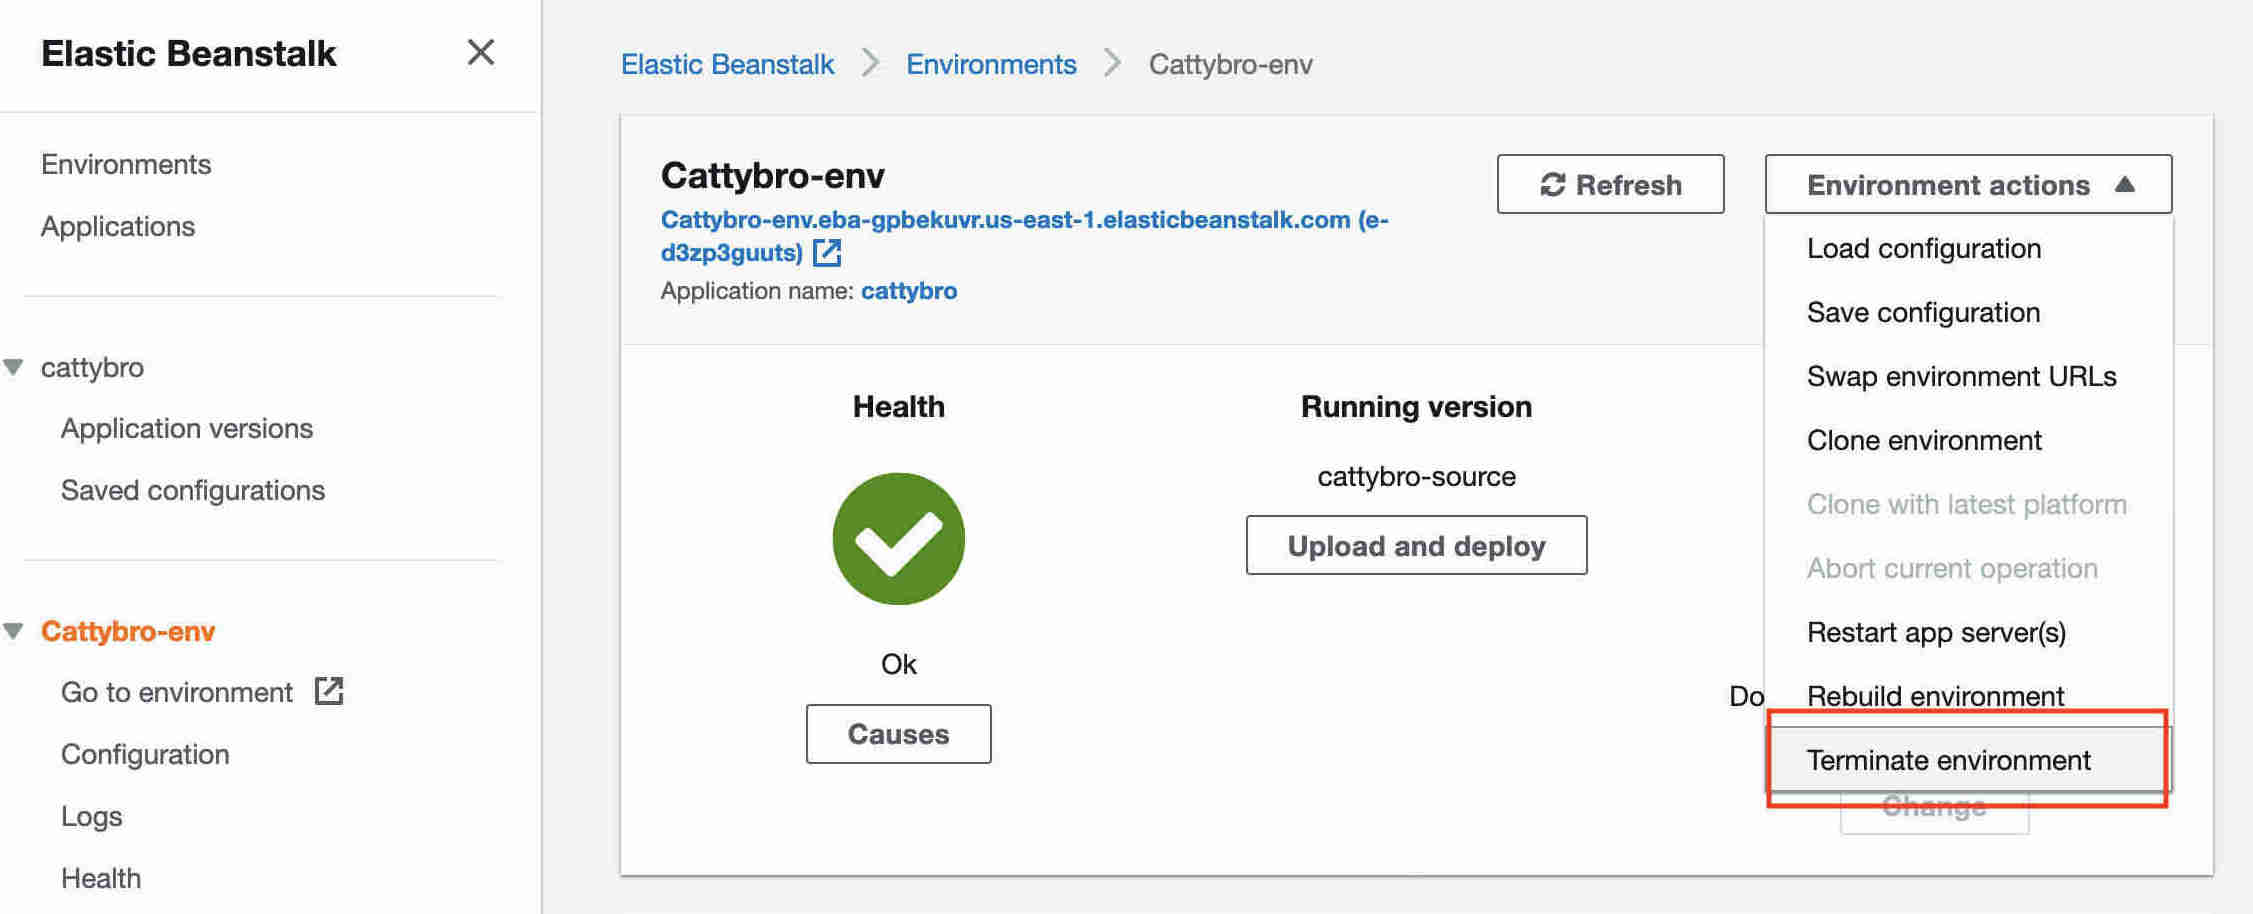
\includegraphics[width=\textwidth]{images/eb-terminate.jpg}
\caption{Terminate EB}
\end{figure}


축하합니다! 첫 번째 Docker 응용 프로그램을 배포했습니다! 많은 단계처럼 보일 수 있지만, EB의 커맨드 라인 도구를 사용하면 Heroku의 기능을 몇 번의 키 스트로크로 거의 모방할 수 있습니다! Docker가 클라우드에서 응용 프로그램을 구축하고 배포하는 많은 어려움을 덜어준다는 것에 동의하시길 바랍니다. AWS의 단일 컨테이너 Docker 환경에 대한 문서를 읽어보시길 권장합니다.

튜토리얼의 마지막 부분에서는 좀 더 복잡한 실제 환경을 모방하는 응용 프로그램을 배포할 것입니다. 영구적인 백엔드 저장소 계층이 있는 앱입니다. 바로 시작해 봅시다!

\chapter{docker 이미지 만들기}
우리는 이제 docker를 이용하여 서버를 설치할 수 있다. 몇번의 명령어를 실행하면 이미 만들어져 있는 서버를 순식간에 만들어낼 수 있다니 놀랍지 않나요? 이번 장에서는 앞에서 설치한 ststic-site를 수정하여 나만의 static site로 만드는 방법을 학습한다. 이 때 중요한 명령어는 commit이다. 

\section{commit하기}
지금 여러분의 컴퓨터에 설치되어 있는 이미지가 어떤 것들이 있는지 살펴보자. 
아래 명령어를 실행하면 현재 다운로드 되어 있는 이미지를 볼 수 있다. 이 이미지를 컨테이너에 넣은 다음 실행해야 서버가 동작한다. `docker images` 를 실행하면 의 이미지가 나열된 결과를 볼수 있고, 지난 시간에 사용하였던 static-site가 보인다. 이 도커 이미지를 컨테이너에 넣고 실행하자. 아래와 같이 실행하면 된다. 이 도커 이미지를 실행시키고 myserver라고 이름 붙인다. 컨테이너를 실행 후 firefox를 열어 http://localhost:8080/ 에 접속하면 웹사이트를 볼 수 있다. 

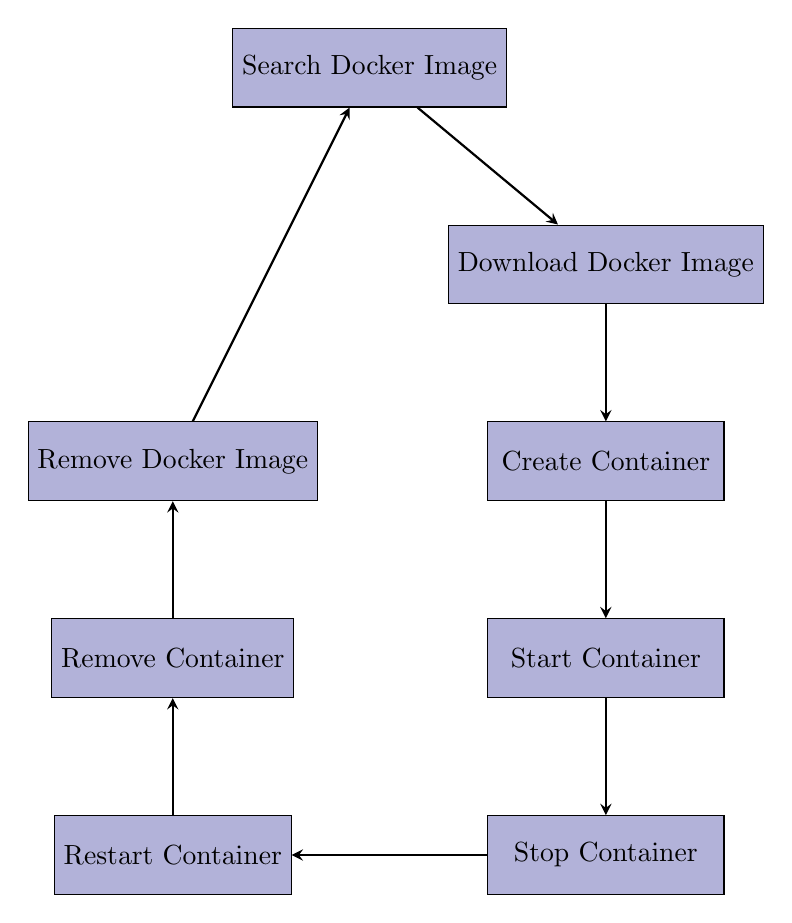
\begin{tikzpicture}[node distance=2.5cm, auto]

    % Nodes
    \node (search) [process] {Search Docker Image};
    \node (download) [process, below of=search, xshift=3cm] {Download Docker Image};
    \node (create) [process, below of=download] {Create Container};
    \node (start) [process, below of=create] {Start Container};
    \node (stop) [process, below of=start] {Stop Container};
    \node (restart) [process, left of=stop, xshift=-3cm] {Restart Container};
    \node (remove) [process, above of=restart] {Remove Container};
    \node (rmi) [process, above of=remove] {Remove Docker Image};

    % Arrows
    \draw [arrow] (search) -- (download);
    \draw [arrow] (download) -- (create);
    \draw [arrow] (create) -- (start);
    \draw [arrow] (start) -- (stop);
    \draw [arrow] (stop) -- (restart);
    \draw [arrow] (restart) -- (remove);
    \draw [arrow] (remove) -- (rmi);
    \draw [arrow] (rmi) -- (search);

\end{tikzpicture}

\begin{lstlisting}[language=Shell]
$ sudo docker images 
REPOSITORY                TAG       IMAGE ID       CREATED         SIZE
mynginx                   latest    3ee48dfc2712   14 hours ago    249MB
nginx                     latest    5ef79149e0ec   12 days ago     188MB
busybox                   latest    65ad0d468eb1   15 months ago   4.26MB
hello-world               latest    d2c94e258dcb   16 months ago   13.3kB
prakhar1989/static-site   latest    f01030e1dcf3   8 years ago     134MB

$ sudo docker run -it -d -p 8080:80 --name myserver prakhar1989/static-site
ec12360056844129f863e79a30869887eee0c4ee87a9e3ea69b2a9aa309af5b0
\end{lstlisting}

이제 이 웹사이트를 수정하려면 컨테이너 안으로 들어가야 한다. 컨테이너에 접속하여 작업을 하기 위해서는 다음과 같은 명령어가 필요하다. 이제 컨테이너 안에서 작업할 수 있다. 작업을 위해 /usr/share/nginx/html/ 이동하고, ls 명령어를 이용하여 파일을 확인한다. 이제 index.html을 수정하여 나만의 홈페이지를 만든다. 
\begin{lstlisting}[language=Shell]
# docker exec -it [container name] /bin/bash
$ sudo docker exec -it myserver /bin/bash
root@ec1236005684:/# 
root@ec1236005684:/# cd /usr/share/nginx/html/
root@ec1236005684:/usr/share/nginx/html# ls
50x.html  css  images  index.html
root@ec1236005684:/usr/share/nginx/html# 
\end{lstlisting}

index.html 파일을 수정하기 위해서 vi 에이터를 사용해 본다. 자신이 익숙한 에디터를 사용해도 된다. vi 에디터가 없다면 cat명령어 사용법을 공부한 후 시도 해본다. 

\begin{figure}[htp]
    \centering
    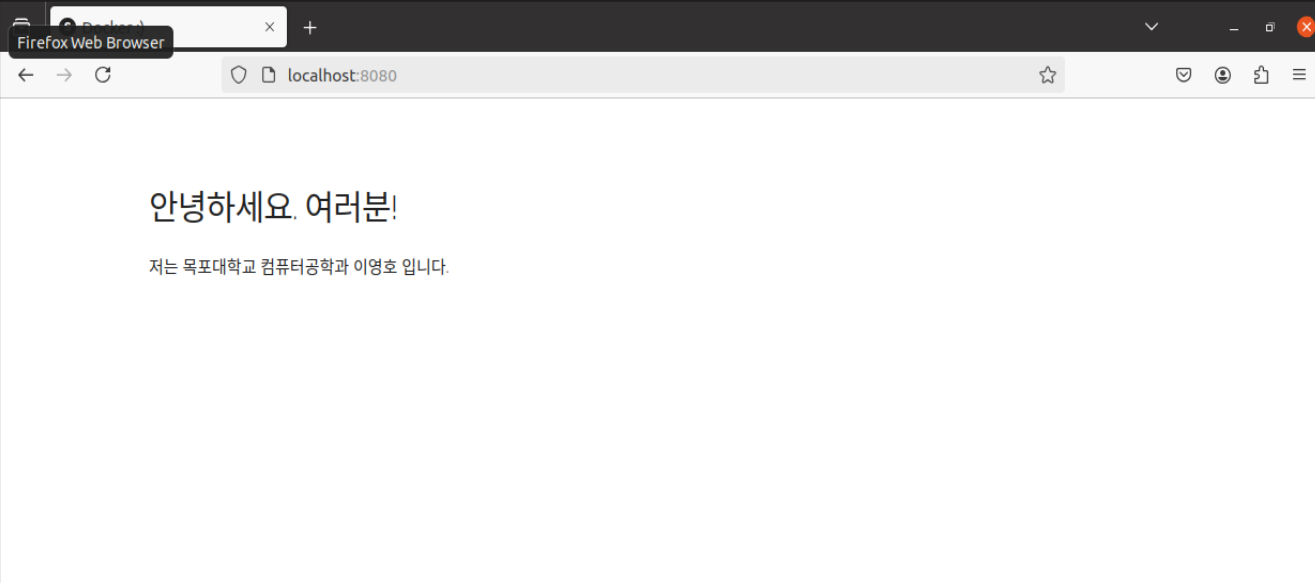
\includegraphics[width=\textwidth]{images/chaptert5images/image.png}
\end{figure}

이제 여러분은 도커 이미지를 받아 새로운 서버를 만들 수 있게 되었다. 하지만 컨테이너는 읽기만 가능하고 쓰기는 불가능하다. 즉, 실행종료 후에 다시 실행하면 여러분의 작업 내용은 삭제된다. 따라서 새로운 도커 이미지, 즉 여러분 만의 도커 이미지를 만들 수 있어야 한다. 

\begin{lstlisting}[language=Shell]
root@ec1236005684:/usr/share/nginx/html# exit
    exit
$ sudo docker stop myserver 
    myserver
$ sudo docker commit myserver mynewserver
sha256:3372a92d9e3f83605e5149ccf794a4b85121f023738f8e76a7d74896e1c199bc
$ sudo docker images
    REPOSITORY                TAG       IMAGE ID       CREATED         SIZE
    mynewserver               latest    3372a92d9e3f   7 seconds ago   134MB
    mynginx                   latest    3ee48dfc2712   14 hours ago    249MB
    nginx                     latest    5ef79149e0ec   12 days ago     188MB
    busybox                   latest    65ad0d468eb1   15 months ago   4.26MB
    hello-world               latest    d2c94e258dcb   16 months ago   13.3kB
    prakhar1989/static-site   latest    f01030e1dcf3   8 years ago     134MB
$ sudo docker run -it -d -p 8080:80 --name myserver2 mynewserver
    b4f7a1fe87876611583293bd0e0beaf9e5ed1facf37ae26f2a1aa83c0819cdcc
\end{lstlisting}

\begin{KnowledgeBox}{도커 이미지 만들기}
    \textbf{영상}
\url{https://www.youtube.com/watch?v=RMNOQXs-f68}
\end{KnowledgeBox}

\chapter{결론}
축하합니다! 이제 Docker를 사용하여 다중 컨테이너 응용 프로그램을 실행하고 배포할 수 있습니다. 이 튜토리얼을 통해 많은 것을 배웠기를 바랍니다. Docker는 매우 강력한 도구이며, 이를 사용하여 프로덕션 응용 프로그램을 쉽게 실행하고 배포할 수 있습니다. 이 튜토리얼에서 다루지 않은 많은 고급 기능이 있으므로 공식 문서를 읽어보시길 권장합니다.

\section{다음 단계는?}
Docker를 배우는 여정을 계속하고 싶다면 다음 단계를 고려해 보세요.
\begin{itemize}
    \item 공식 문서를 읽어보세요. Docker에는 매우 잘 작성된 문서가 있습니다.
    \item Docker를 사용하여 더 많은 응용 프로그램을 실행해 보세요. 연습할수록 더 잘할 수 있습니다.
    \item 프로덕션 환경에서 Docker를 사용해 보세요. Docker를 사용하여 프로덕션 응용 프로그램을 실행하면 많은 것을 배울 수 있습니다.
\end{itemize}

\chapter*{부록}
\addcontentsline{toc}{chapter}{부록} % 부록을 목차에 추가
\section*{맥OS용 가상 머신 UTM 설정하기}
\addcontentsline{toc}{section}{맥OS용 가상 머신 UTM 설정하기} % 부록의 섹션도 목차에 추가
여러분이 맥북을 소유하고 있으며, 맥북에 가상머신을 설치하여 실습을 하고 싶다면 UTM을 사용하세요. 애플 실리콘이 장착된 맥북에서는 버추얼 박스를 사용하지 못합니다. UTM은 iOS나 맥OS 에서 실행되는 가상 머신입니다. UTM을 사용하면 맥OS 기기에서 Linux, Windows, FreeBSD, Solaris, Haiku OS 등을 실행할 수 있습니다. UTM을 사용하면 iOS 기기에서 Docker를 실행할 수 있습니다. 

UTM은 항상 완전히 무료이고 오픈 소스입니다. Mac App Store 버전은 GitHub 버전과 동일하며, 누락된 기능은 없습니다. Mac App Store 버전의 유일한 이점은 자동 업데이트를 받을 수 있다는 것입니다. App Store 버전을 구매하면 UTM 개발에 직접적인 자금을 제공하며, 당신의 지지를 표현할 수 있습니다.

UTM을 사용하려면 다음 단계를 따르세요:
\begin{enumerate}
    \item UTM 앱을 다운로드하고 설치하세요. download from github(무료)를 선택하세요. \\$https://docs.getutm.app/installation/macos/$
    \item 우분투 20.04 LTS 이미지를 다운로드하세요. \\$https://ubuntu.com/download/desktop$
    \item UTM 앱을 실행하고, 아래 그림과 같이 "+" 버튼을 눌러 새 가상 머신을 추가하세요. (우분투 20.04 LTS를 선택하세요.)
    \item 가상 머신을 추가하면, 아래 그림과 같이 설정을 변경하세요.
    \item 가상 머신을 시작하고, 아래 그림과 같이 가상 머신에 접속하세요.
\end{enumerate}

\subsection{UTM을 이용하여 Ubuntu 설치하기}

\begin{figure}[htbp]
    \centering
    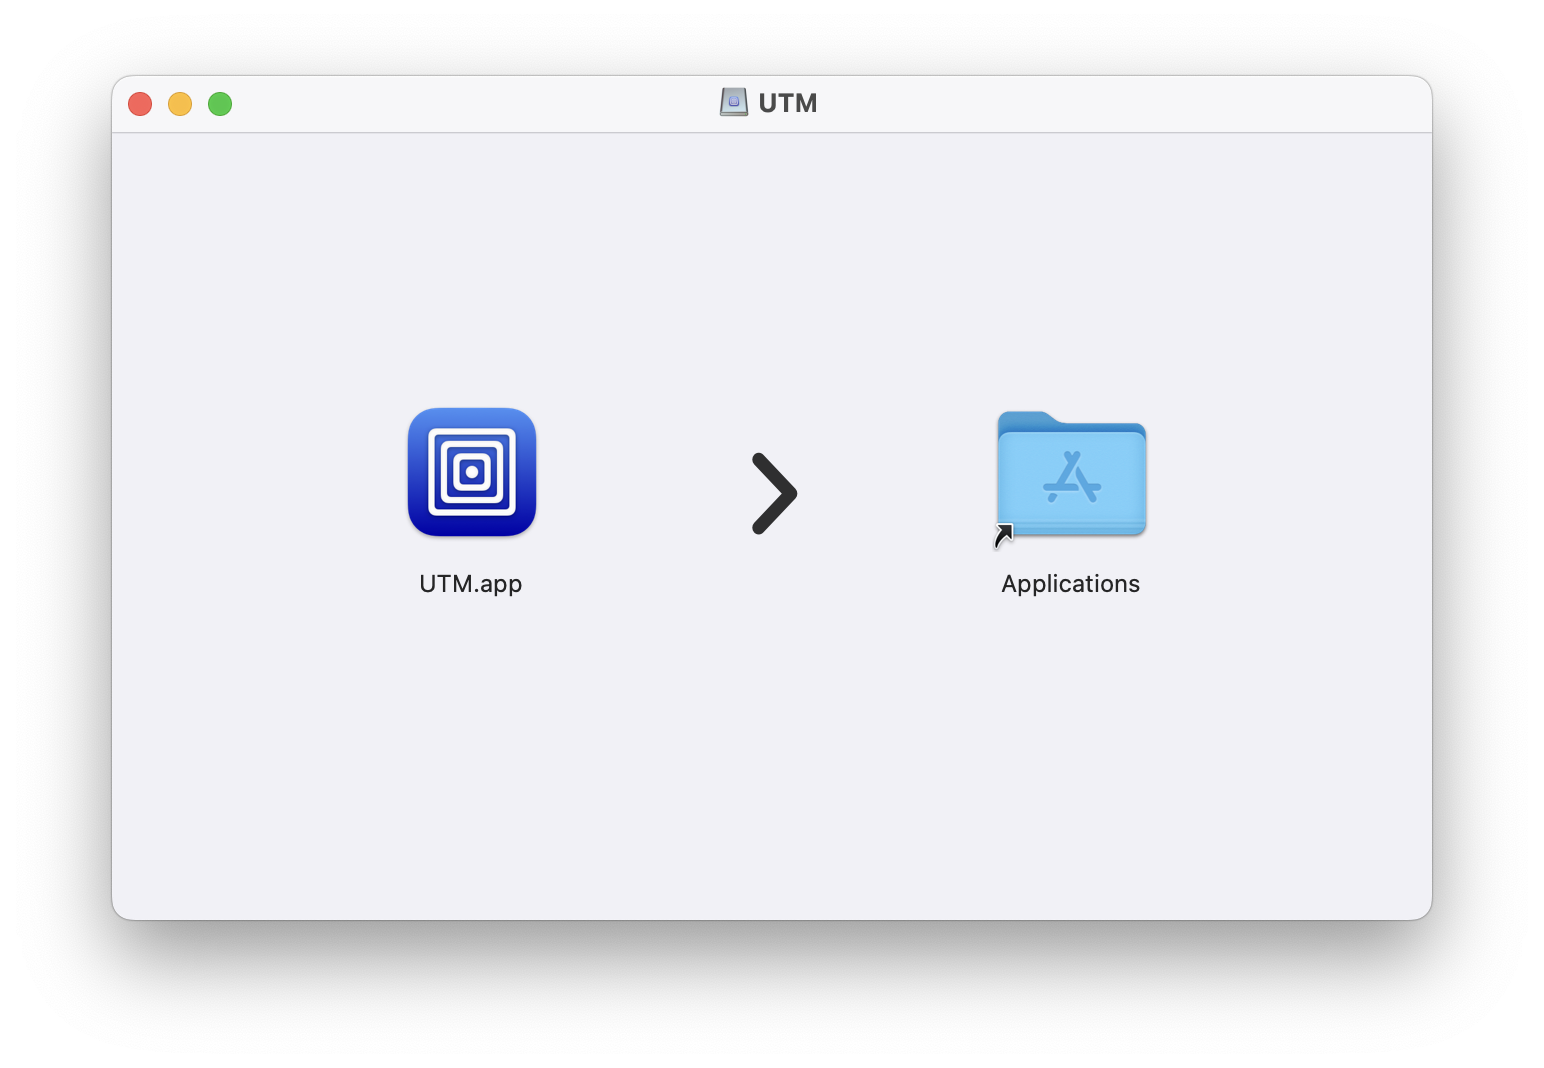
\includegraphics[width=0.9\textwidth]{images/chapter2Images/ch2_image_01.png}
    \caption{설치 프로세스 시작}
\end{figure}

\begin{figure}[htbp]
    \centering
    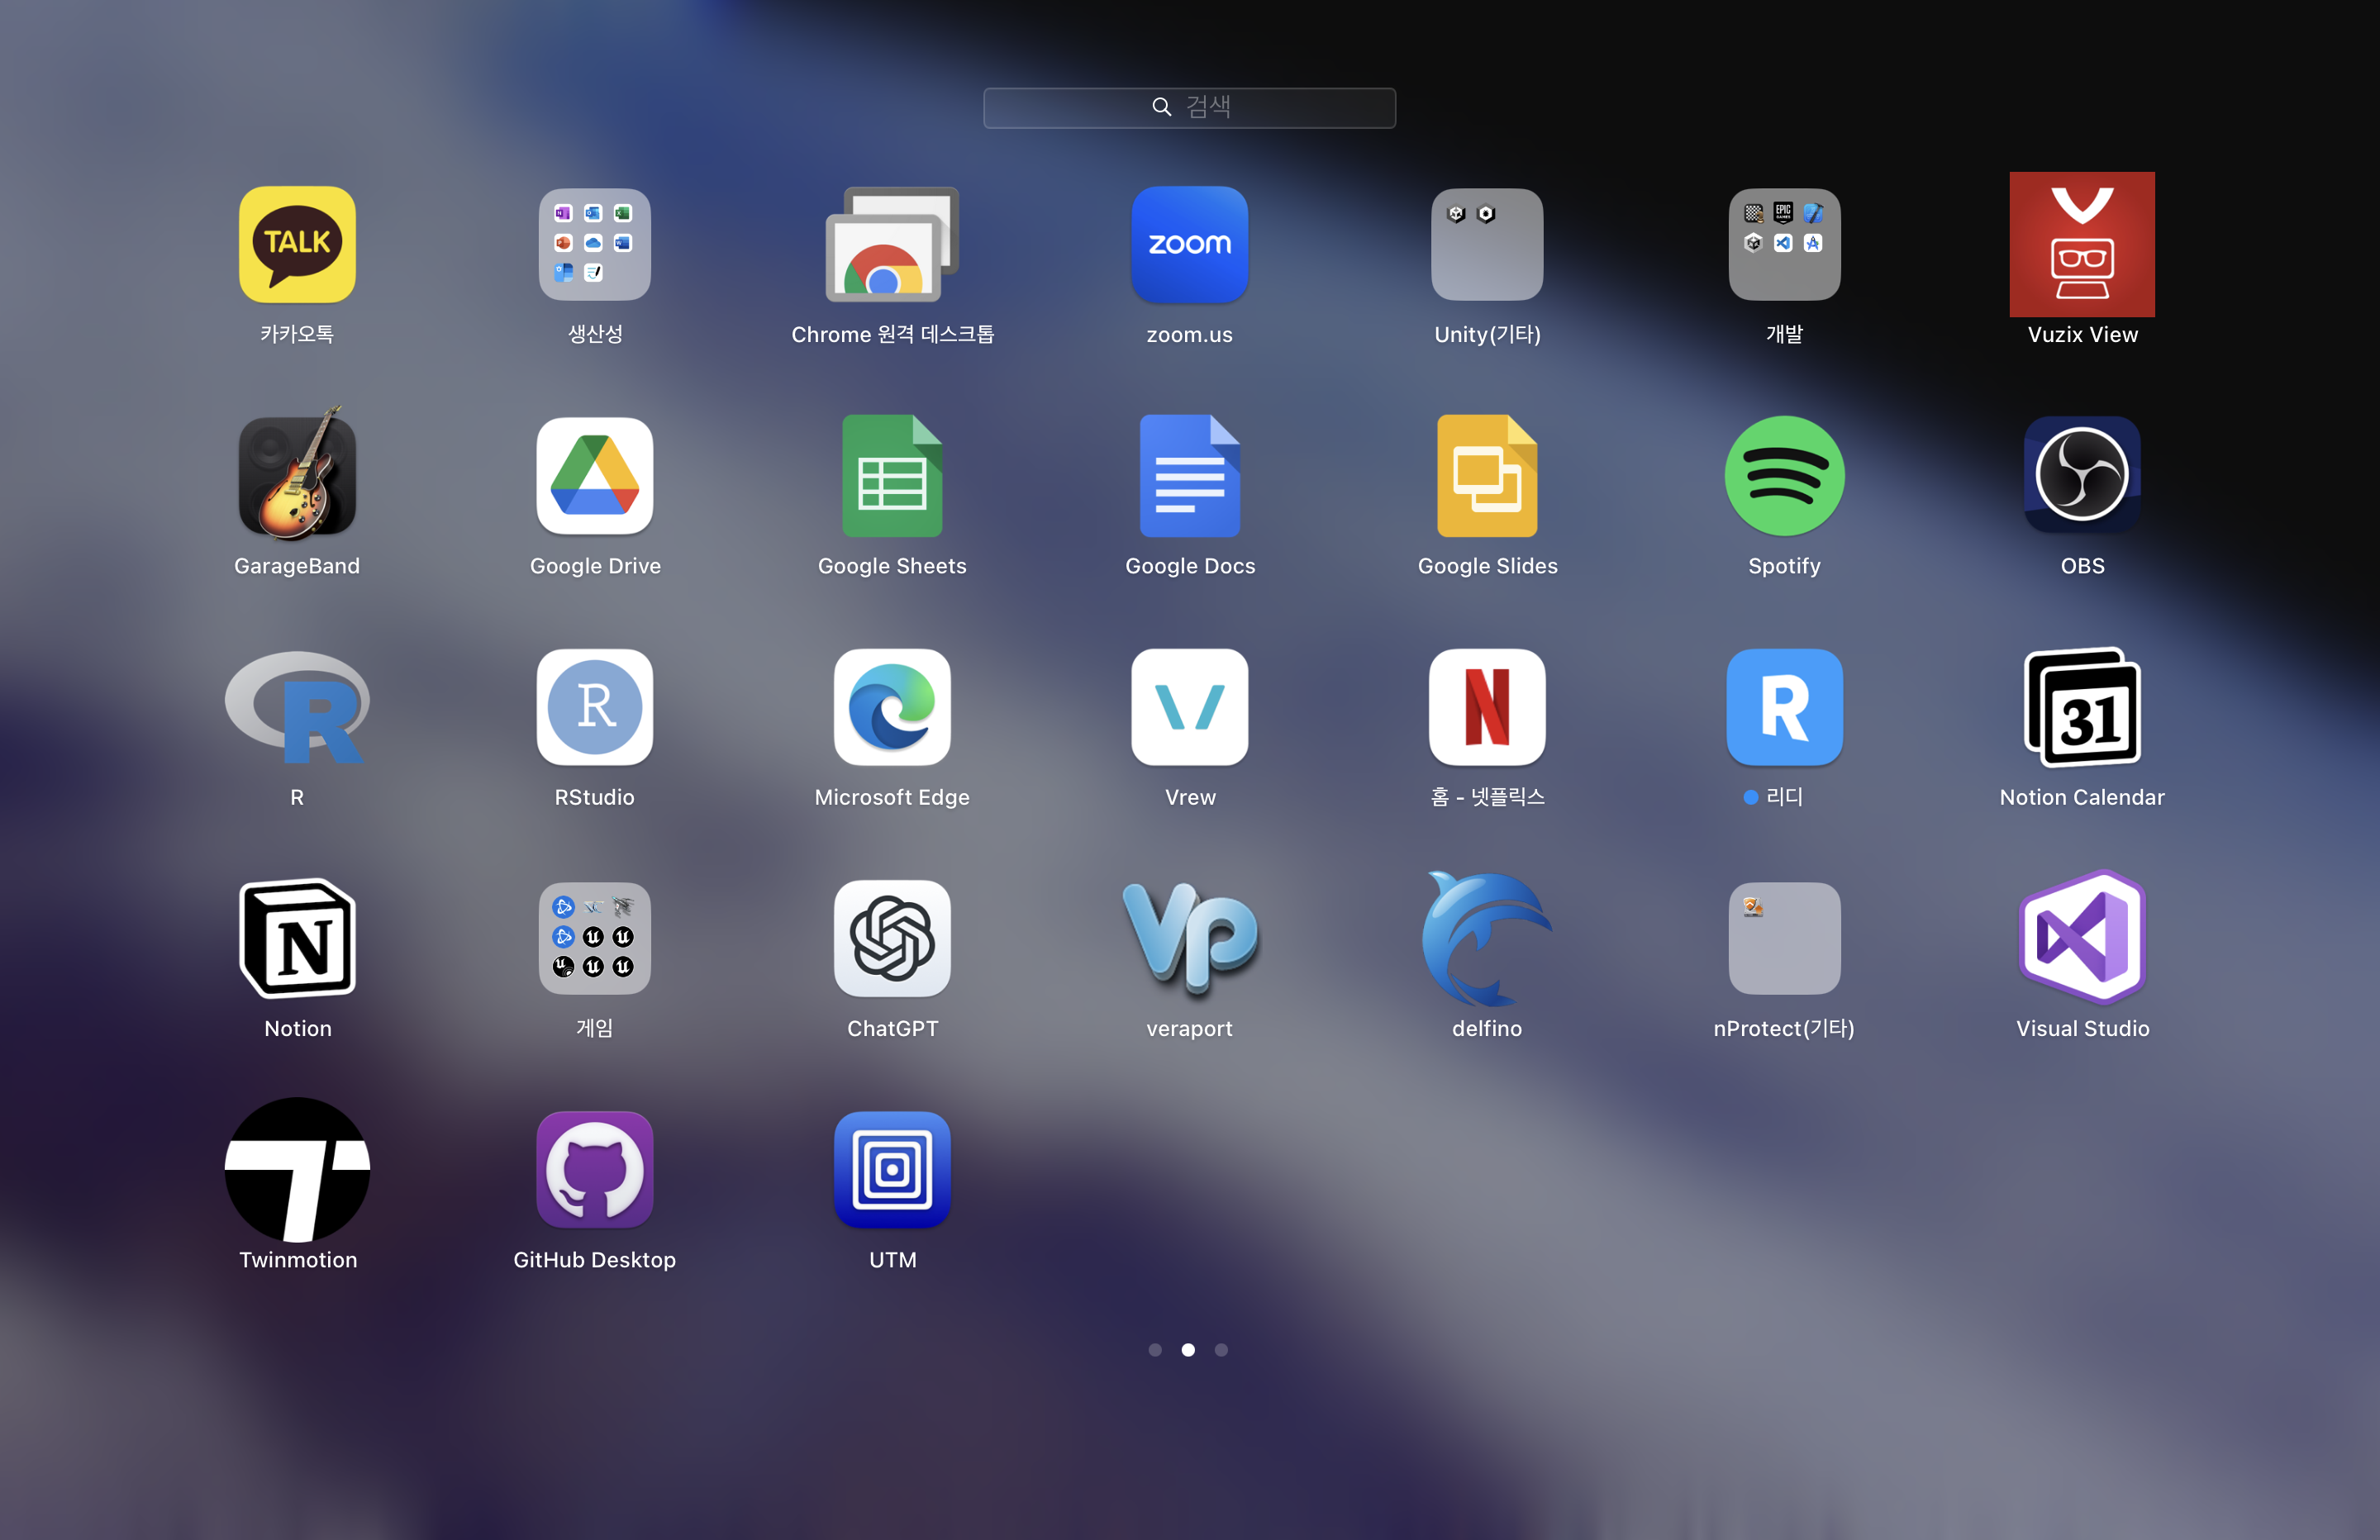
\includegraphics[width=0.9\textwidth]{images/chapter2Images/ch2_image_02.png}
    \caption{설치 언어 선택}
\end{figure}

\begin{figure}[htbp]
    \centering
    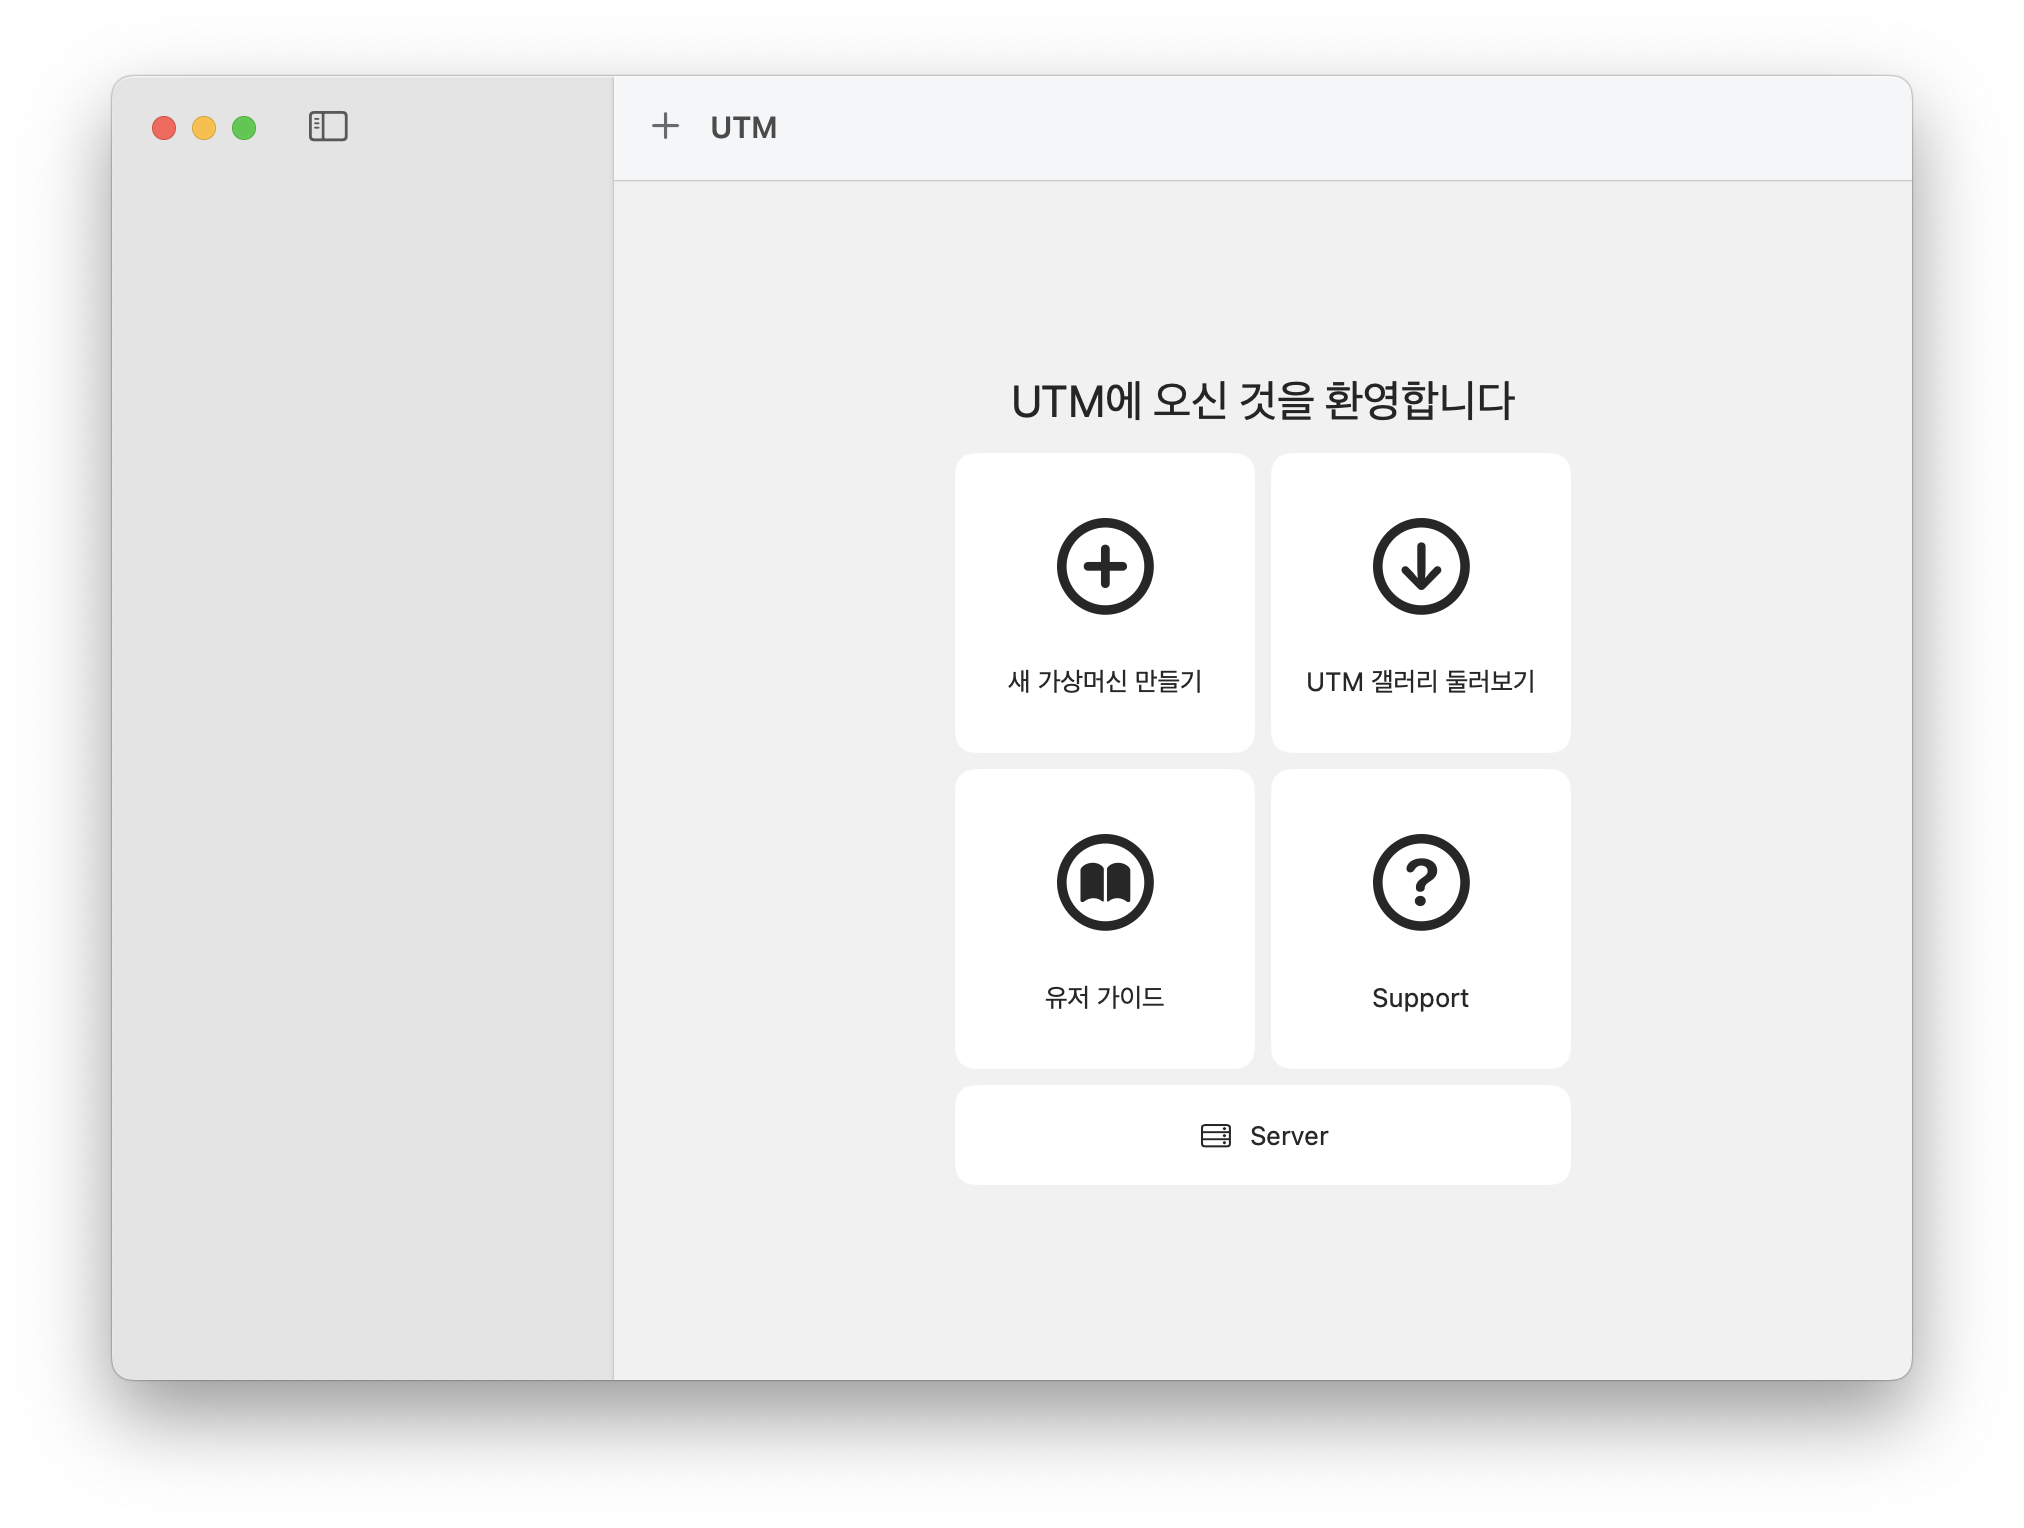
\includegraphics[width=0.9\textwidth]{images/chapter2Images/ch2_image_03.png}
    \caption{설치 준비}
\end{figure}

\begin{figure}[htbp]
    \centering
    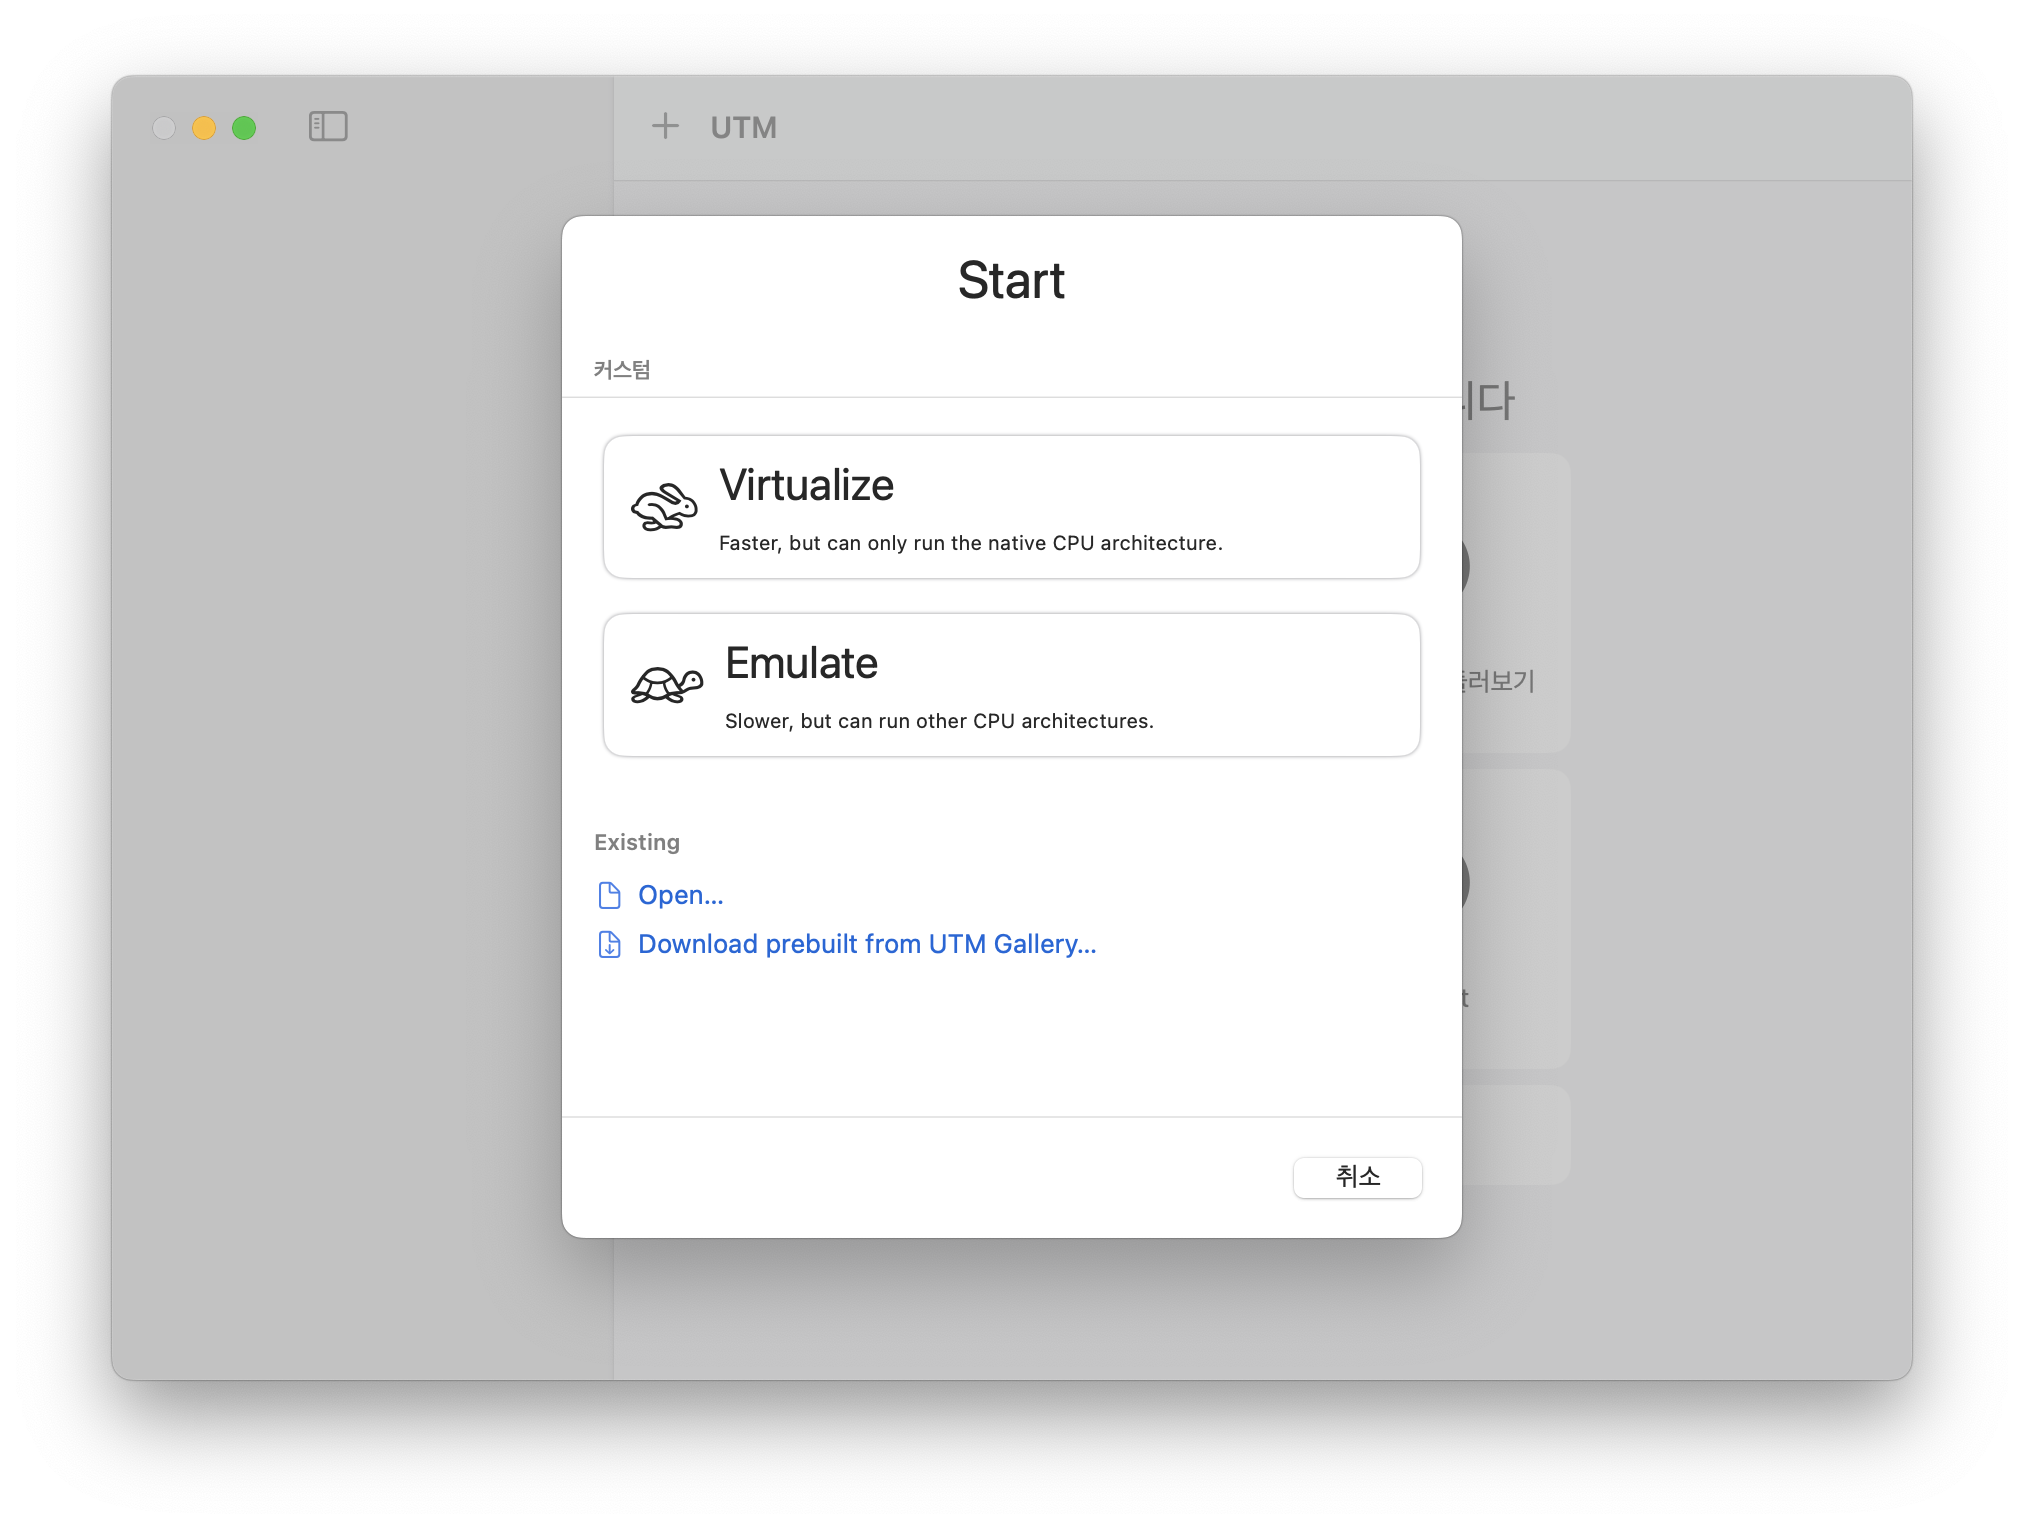
\includegraphics[width=0.9\textwidth]{images/chapter2Images/ch2_image_04.png}
    \caption{시스템 구성}
\end{figure}

\begin{figure}[htbp]
    \centering
    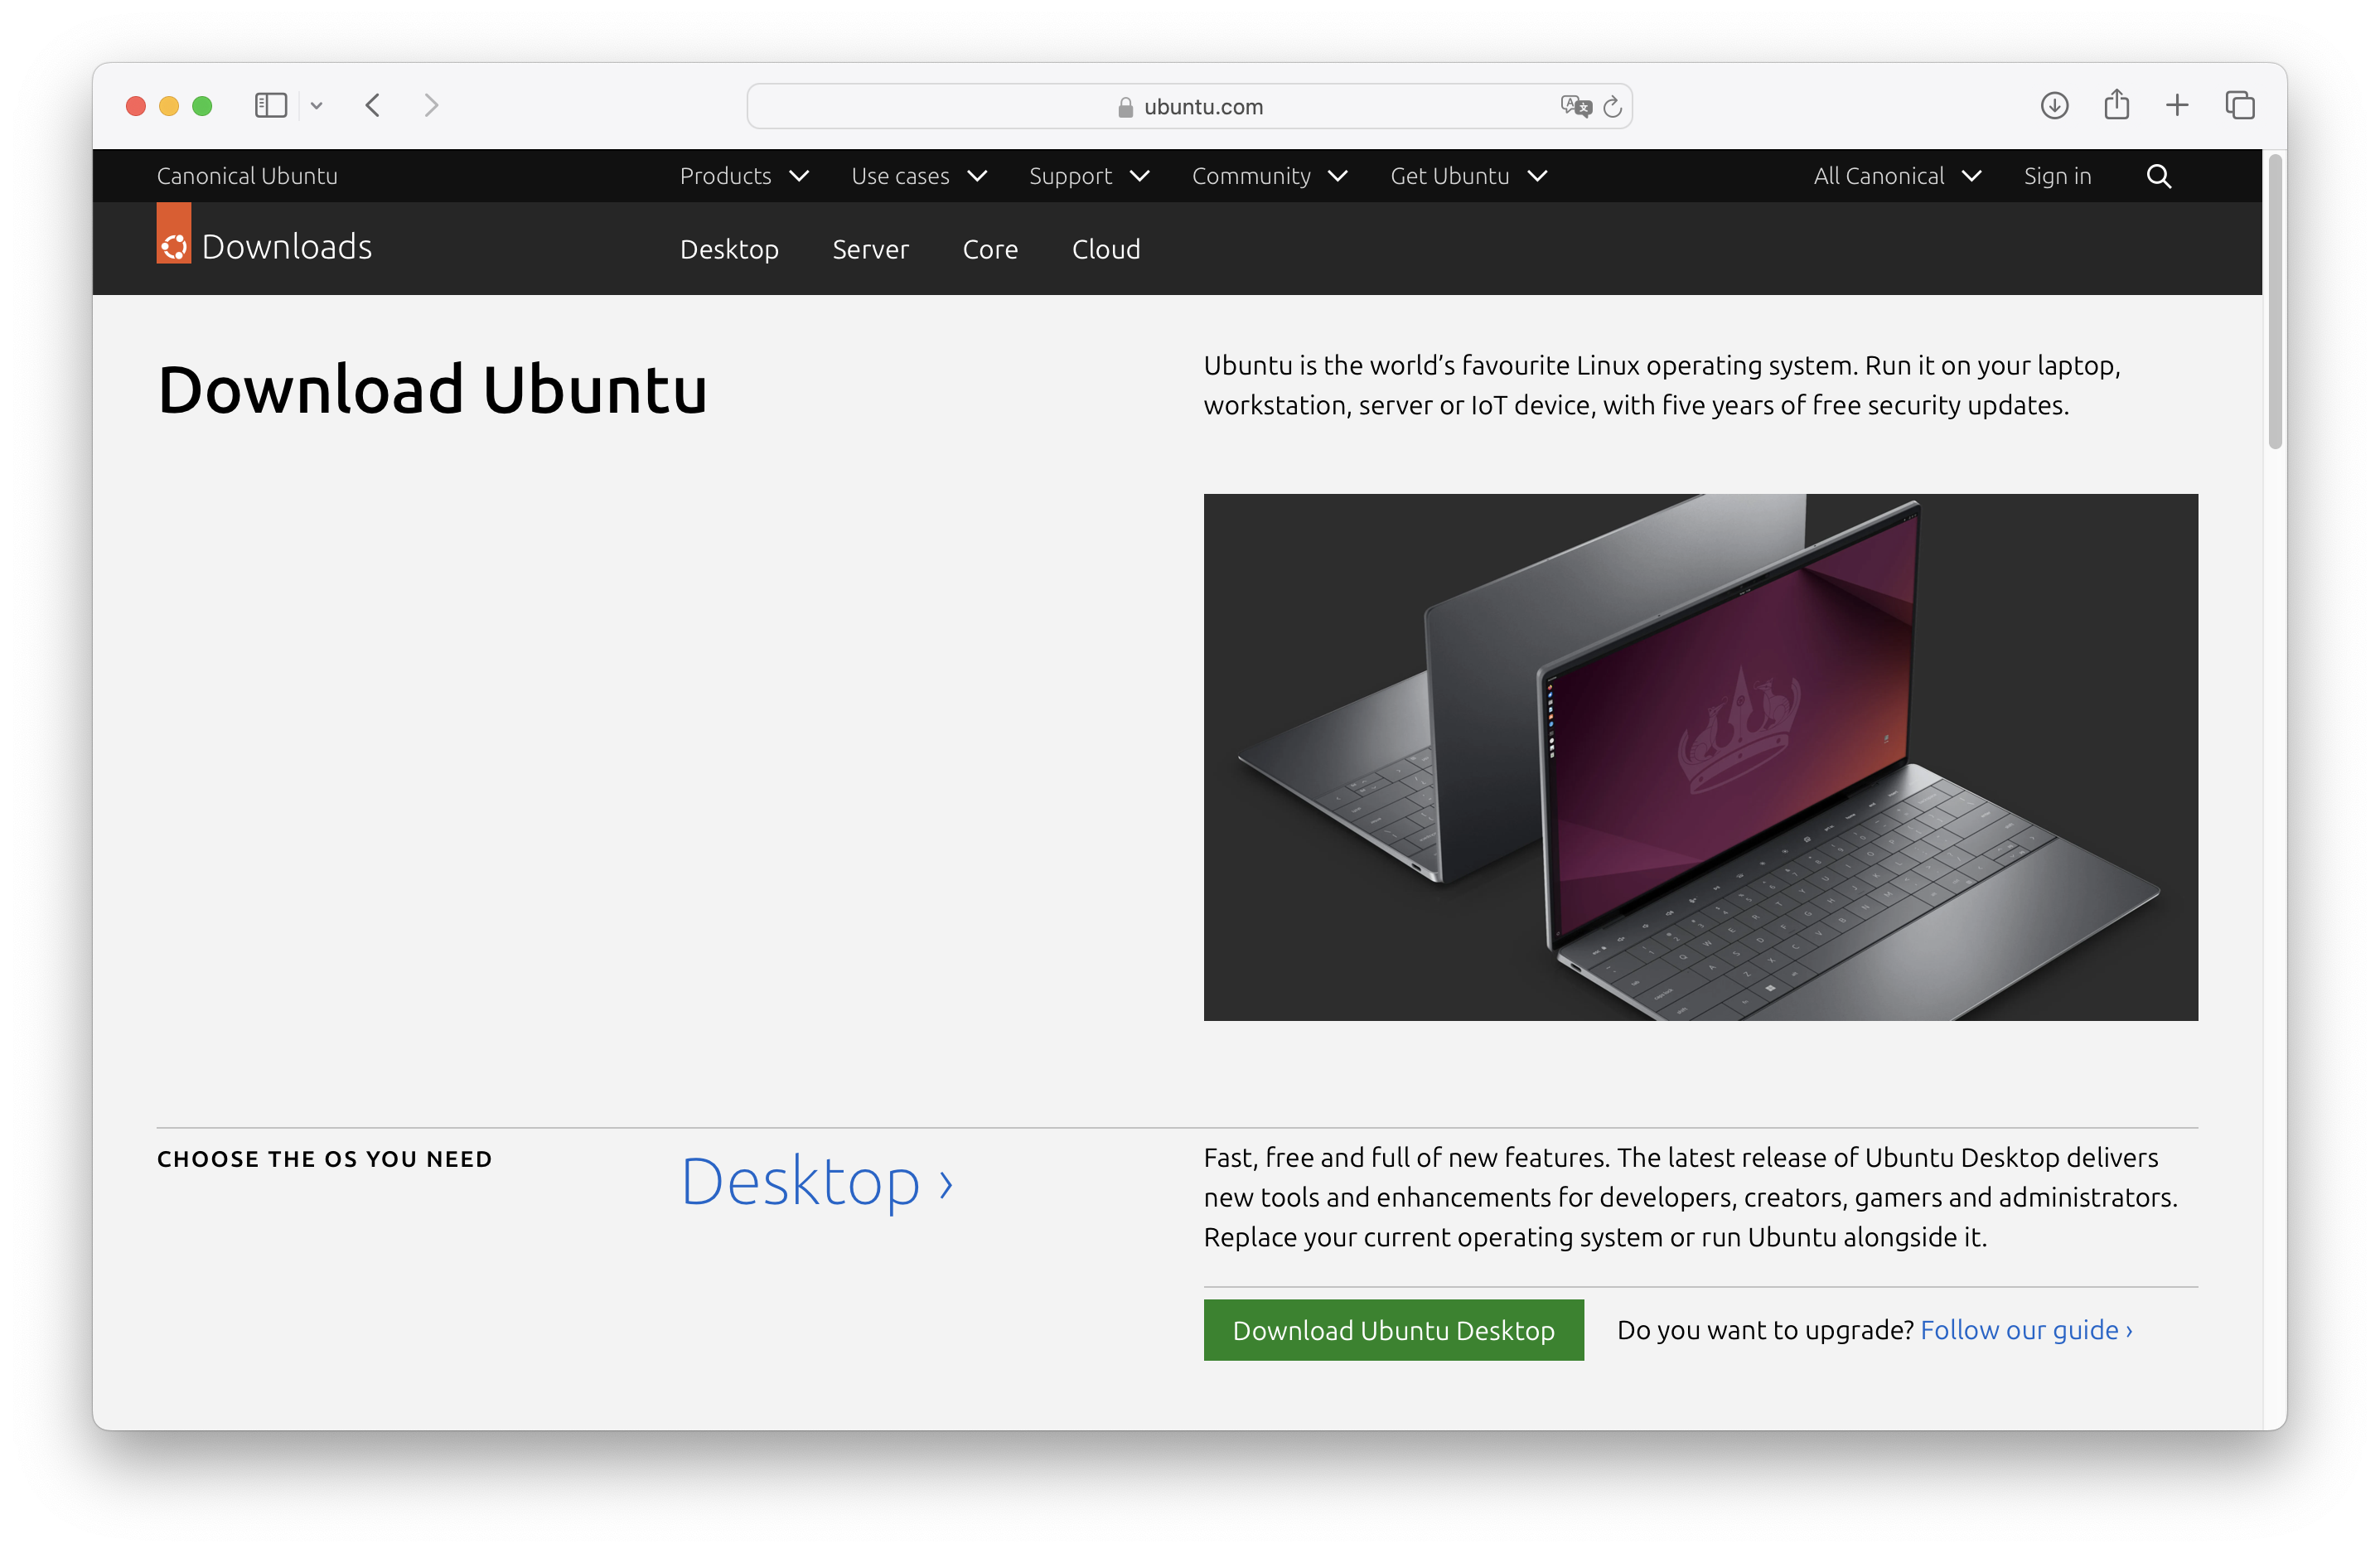
\includegraphics[width=0.9\textwidth]{images/chapter2Images/ch2_image_05.png}
    \caption{시스템 파일 설치}
\end{figure}

\begin{figure}[htbp]
    \centering
    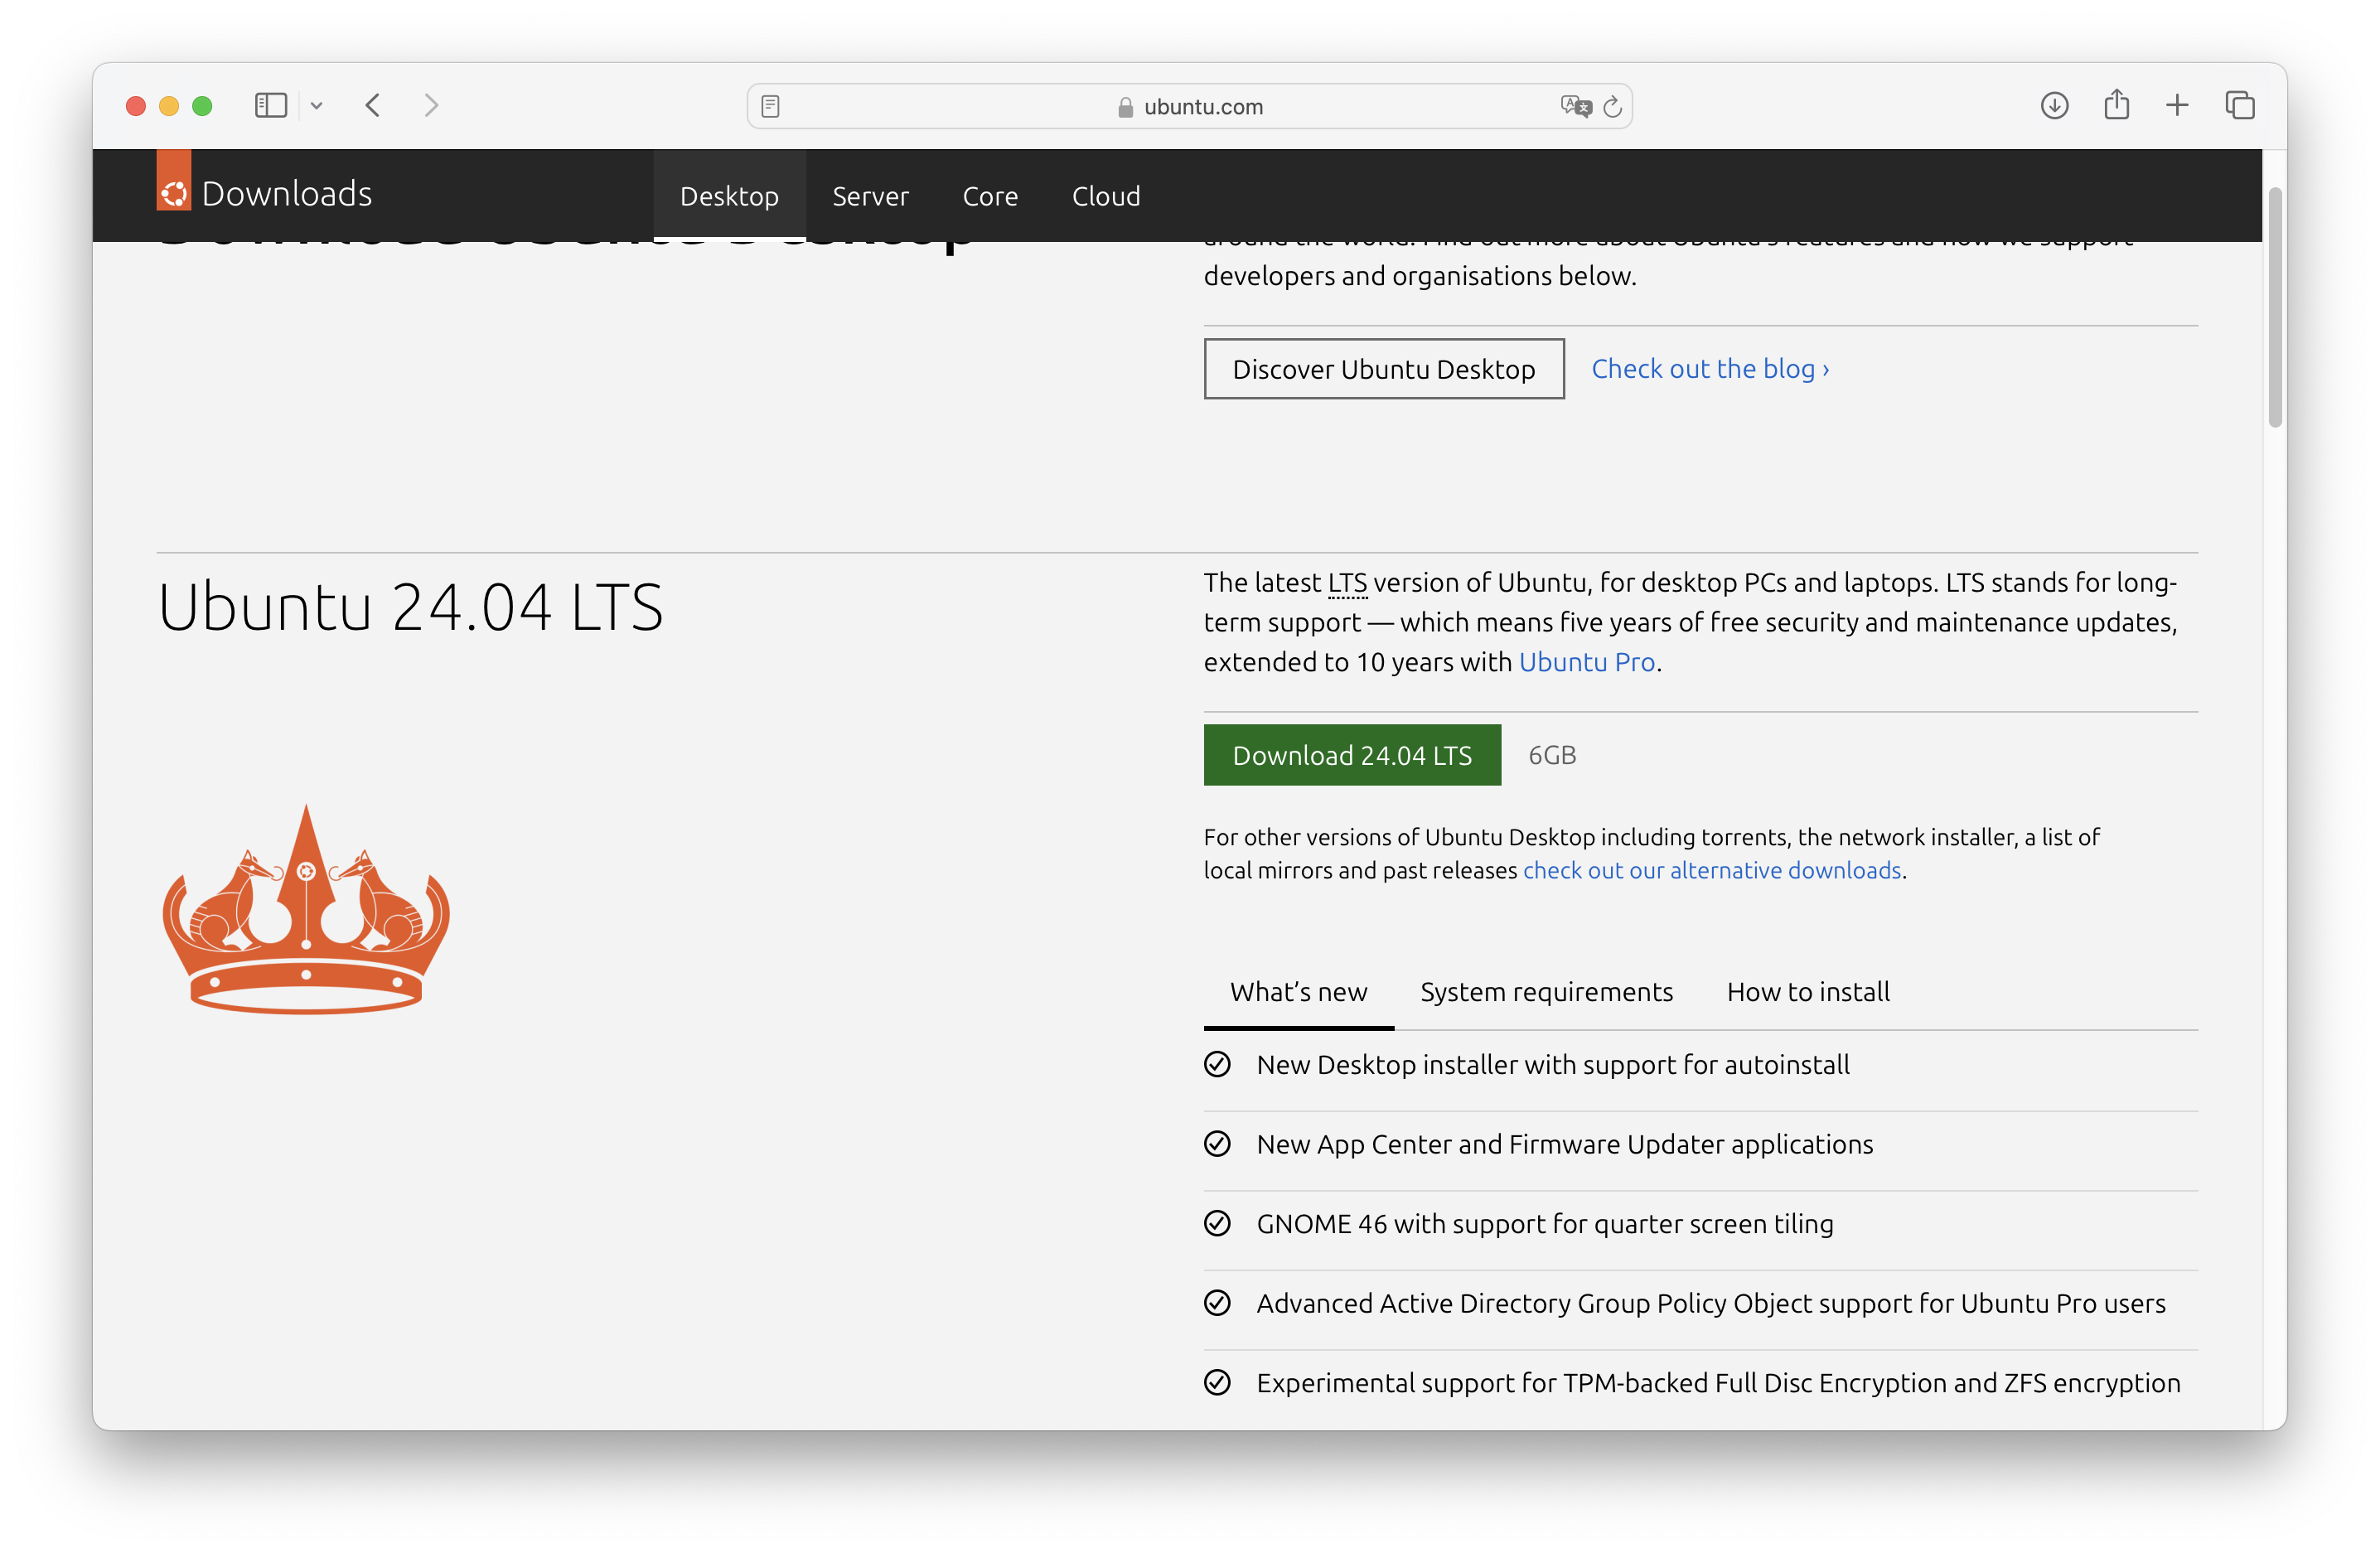
\includegraphics[width=0.9\textwidth]{images/chapter2Images/ch2_image_06.png}
    \caption{설치 완료}
\end{figure}

\begin{figure}[htbp]
    \centering
    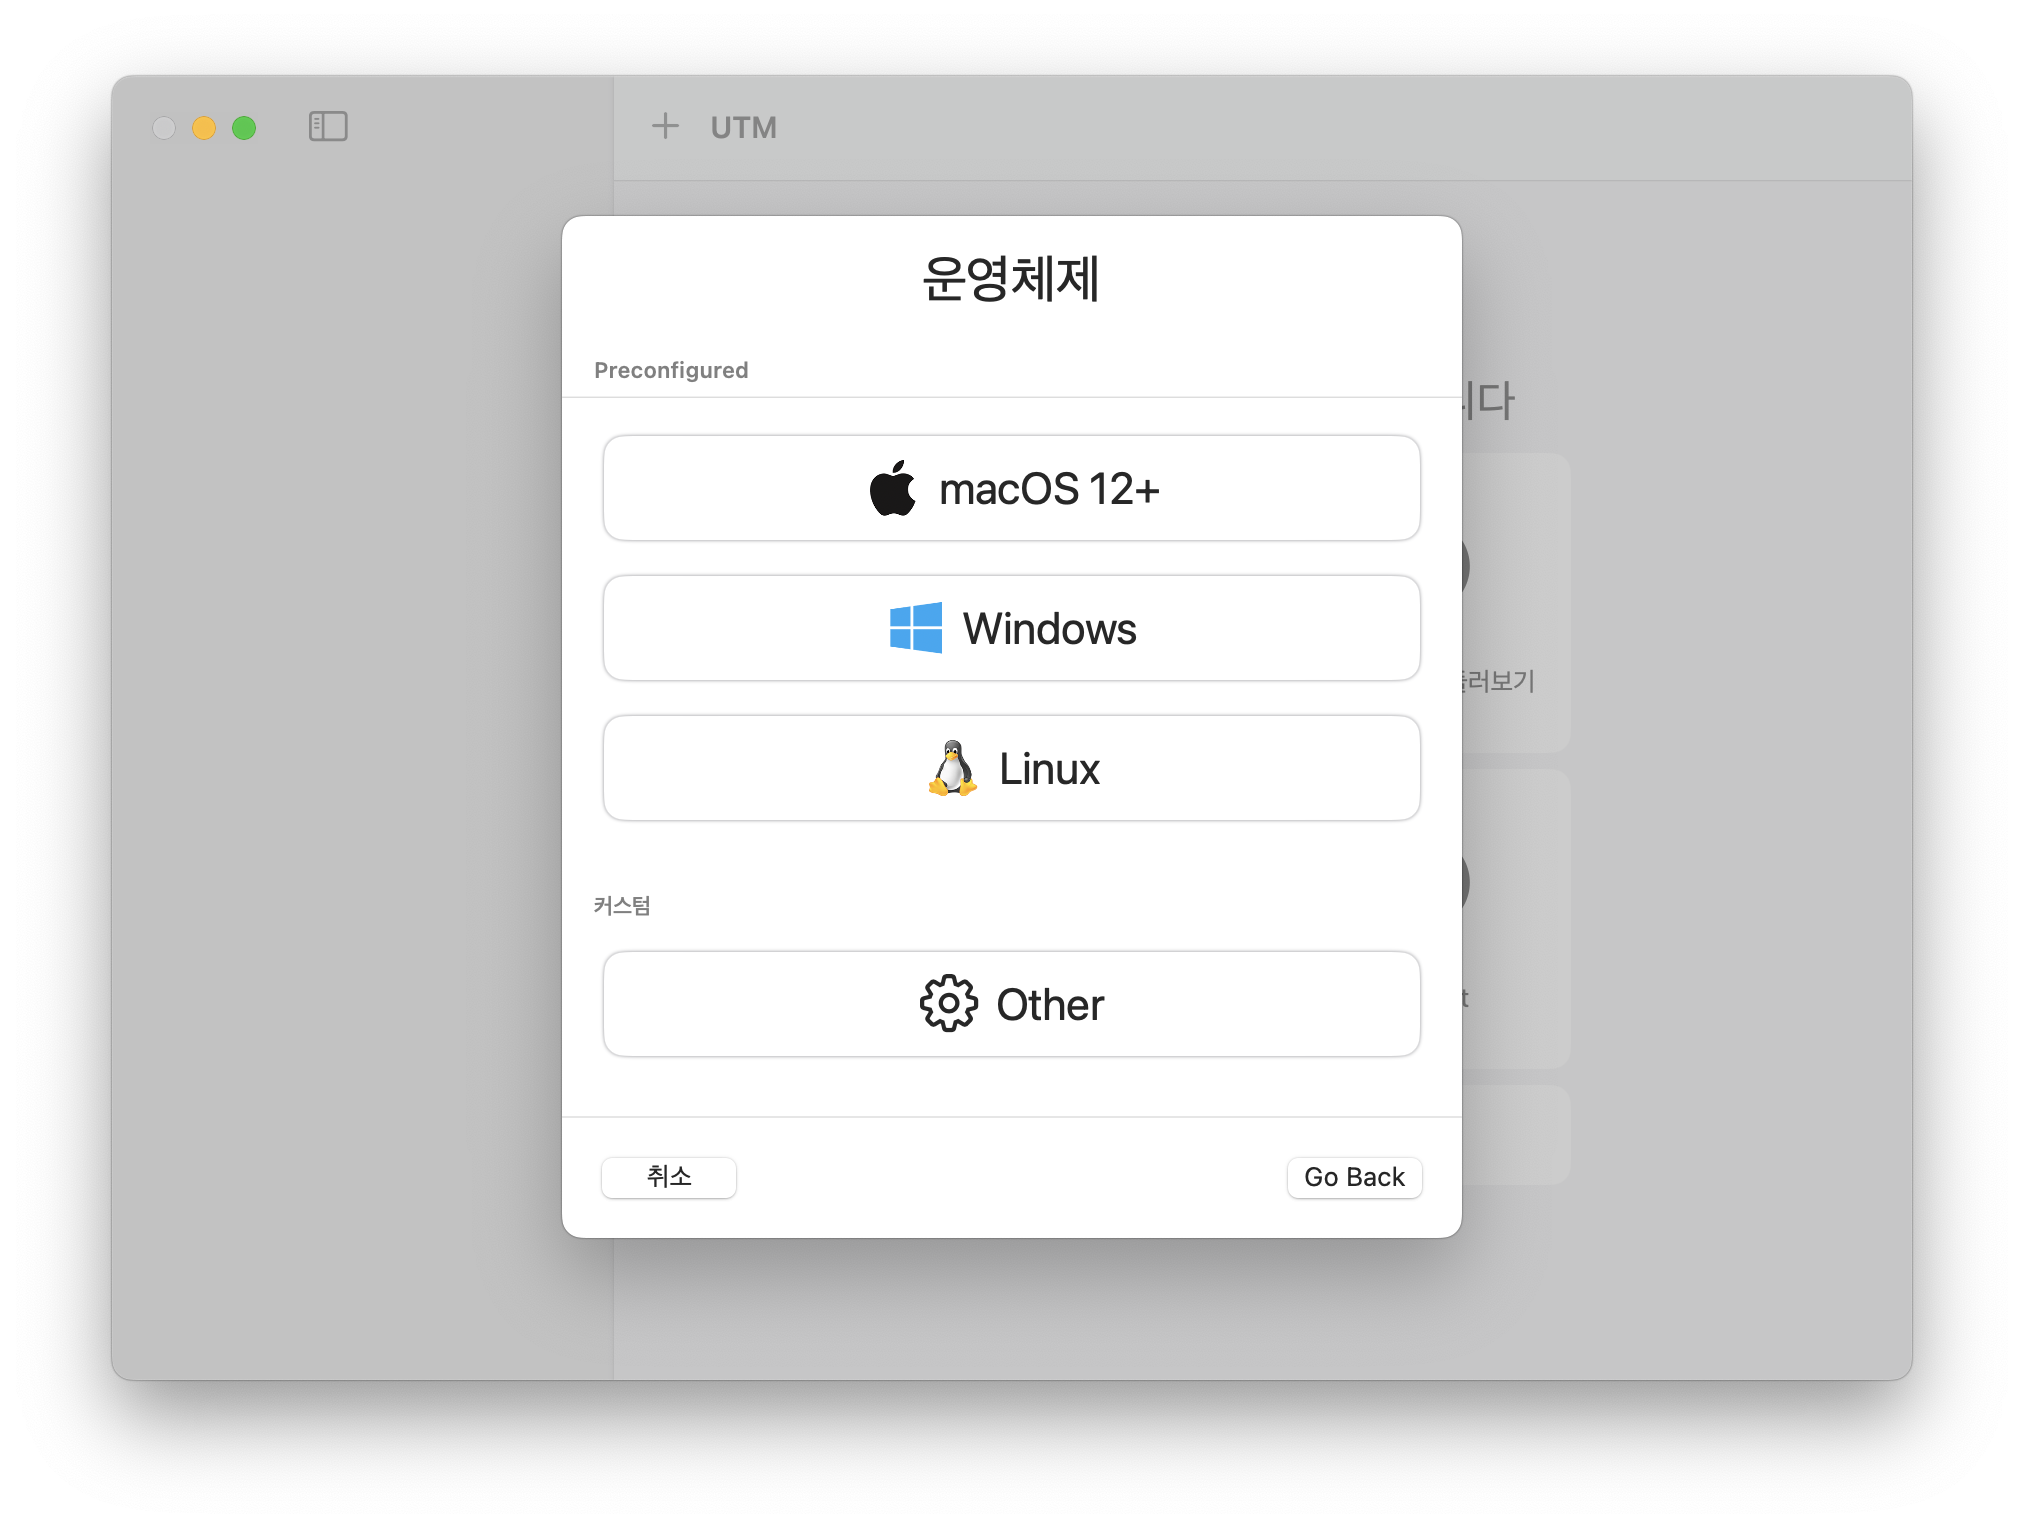
\includegraphics[width=0.9\textwidth]{images/chapter2Images/ch2_image_07.png}
    \caption{시스템 재시작}
\end{figure}

\begin{figure}[htbp]
    \centering
    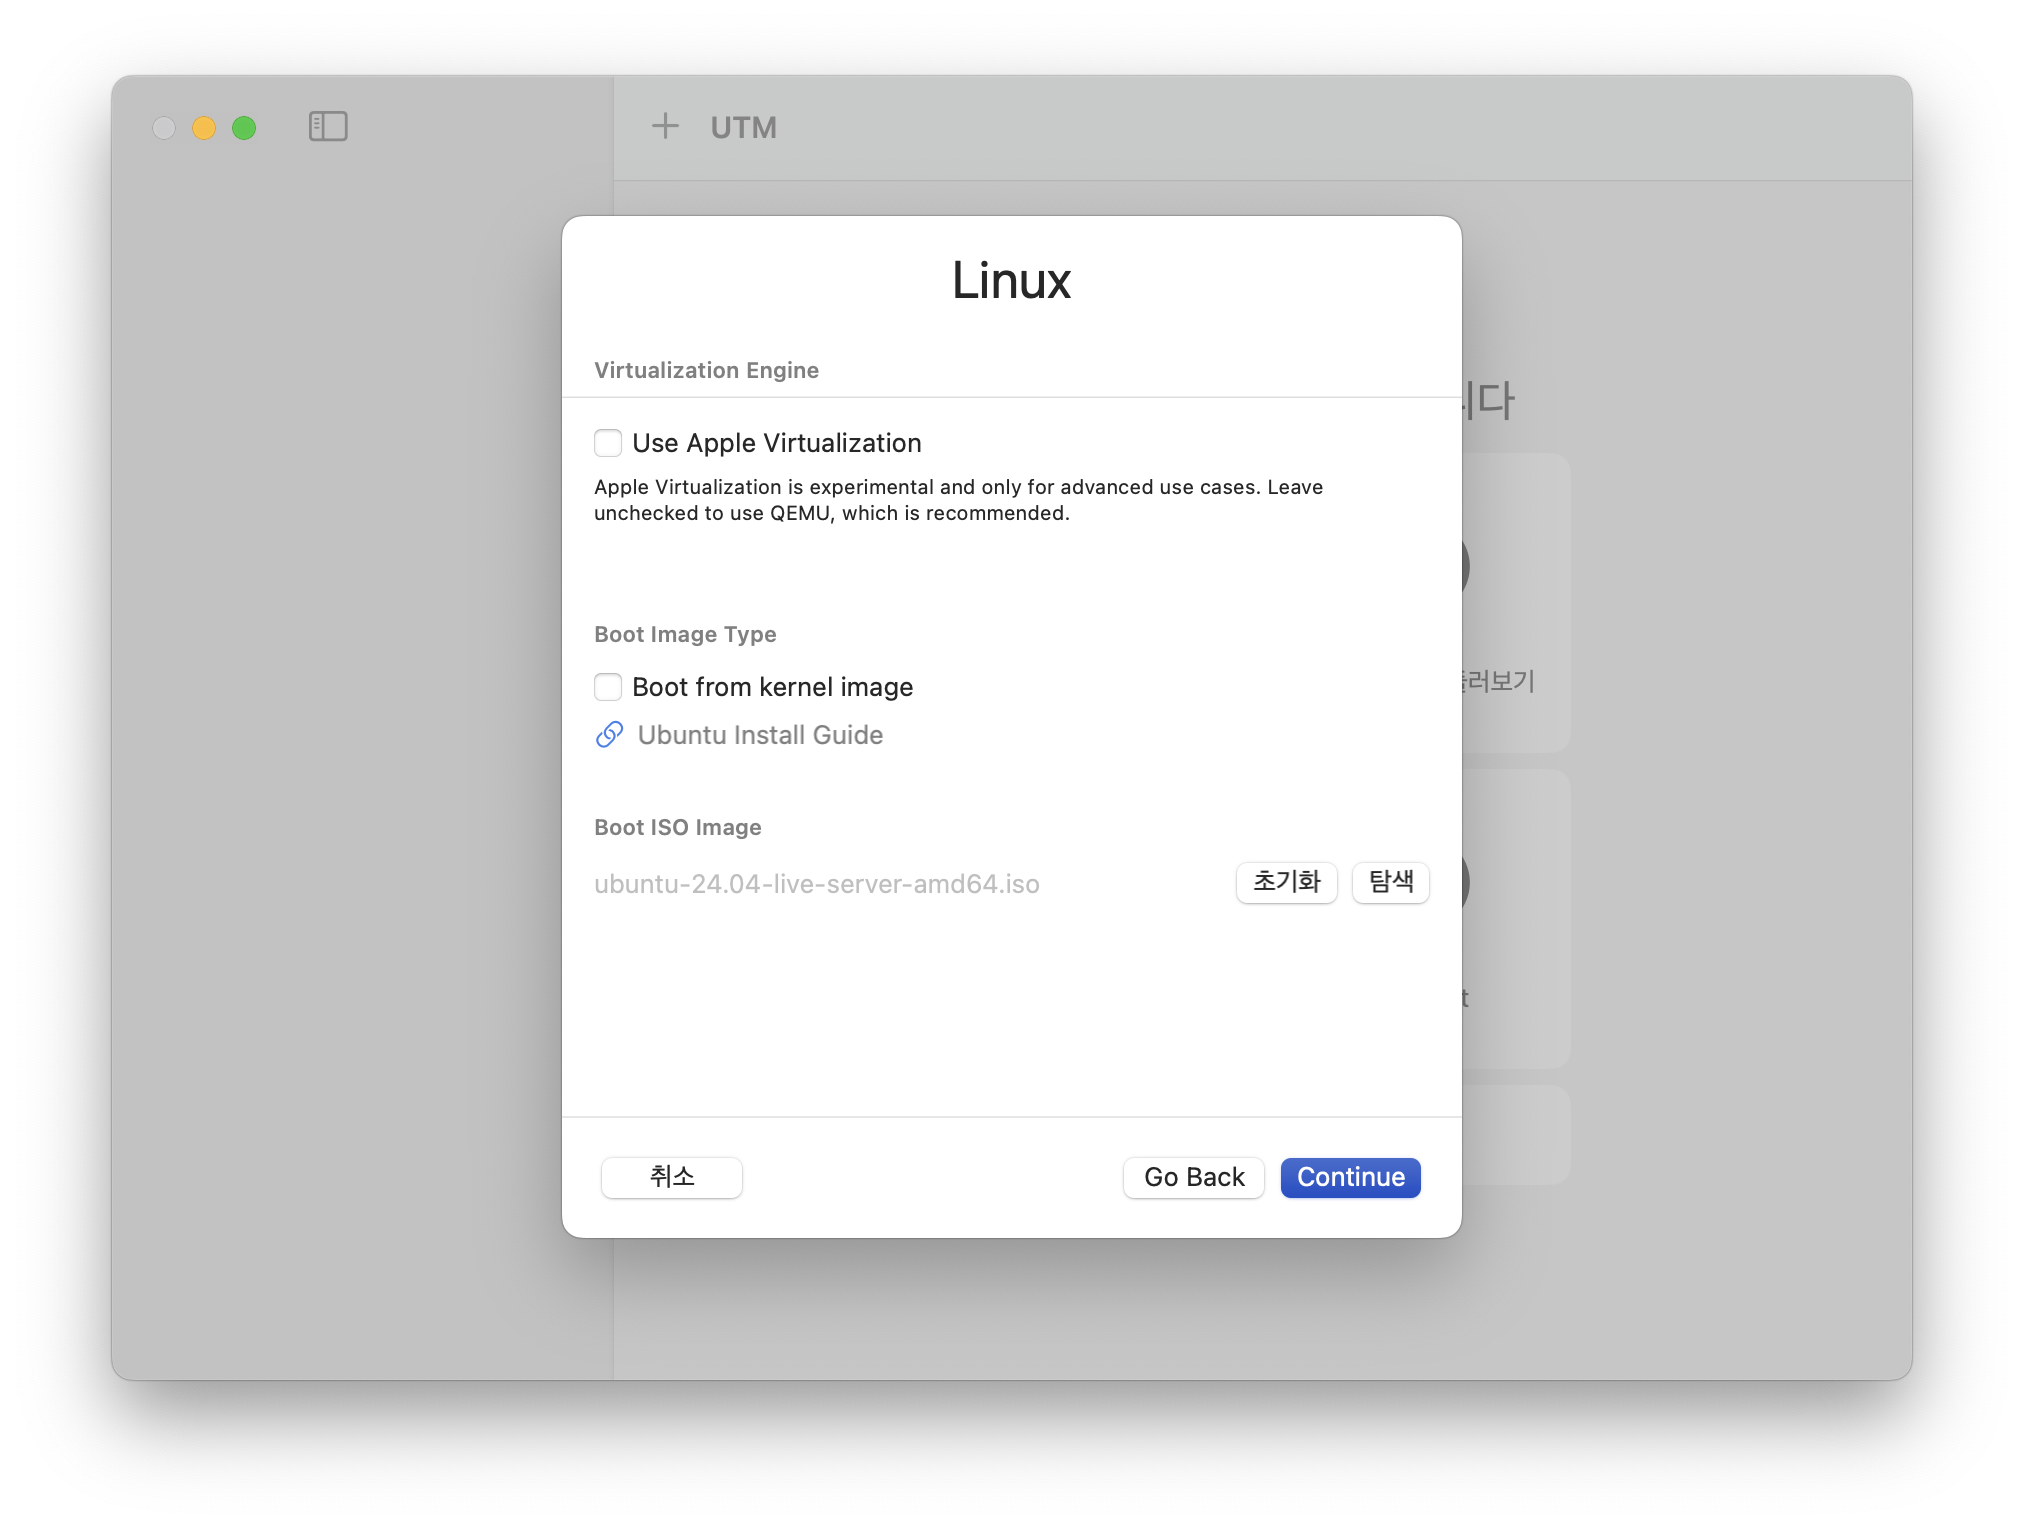
\includegraphics[width=0.9\textwidth]{images/chapter2Images/ch2_image_08.png}
    \caption{설정 완료}
\end{figure}

\begin{figure}[htbp]
    \centering
    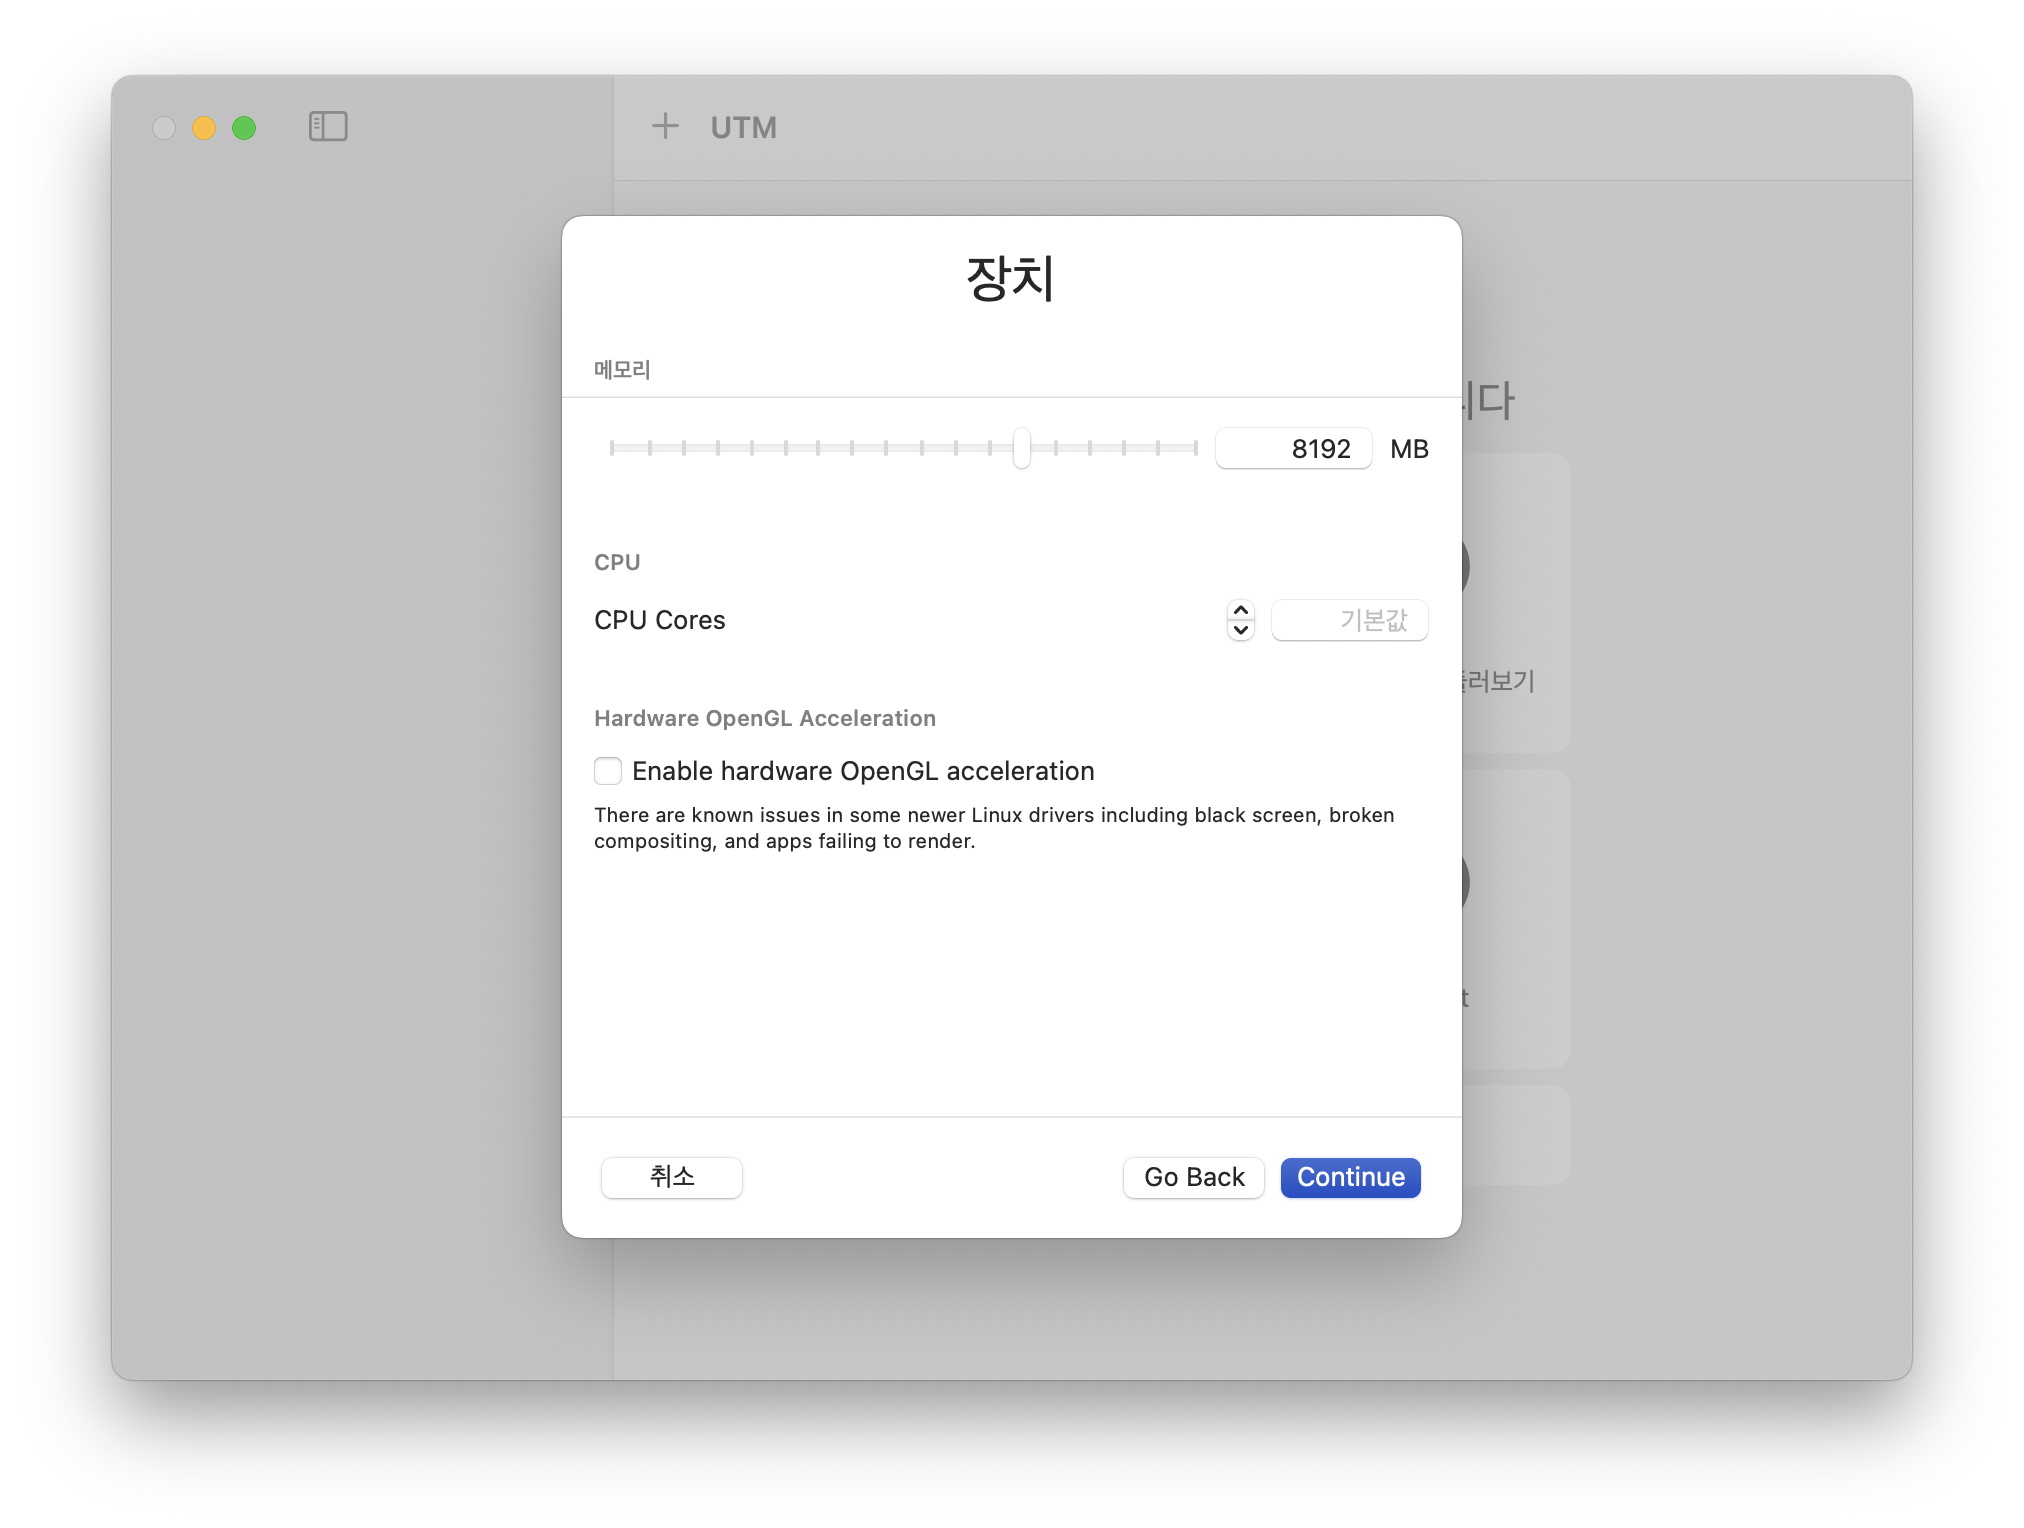
\includegraphics[width=0.9\textwidth]{images/chapter2Images/ch2_image_09.png}
    \caption{초기 Ubuntu 로그인 화면}
\end{figure}

\begin{figure}[htbp]
    \centering
    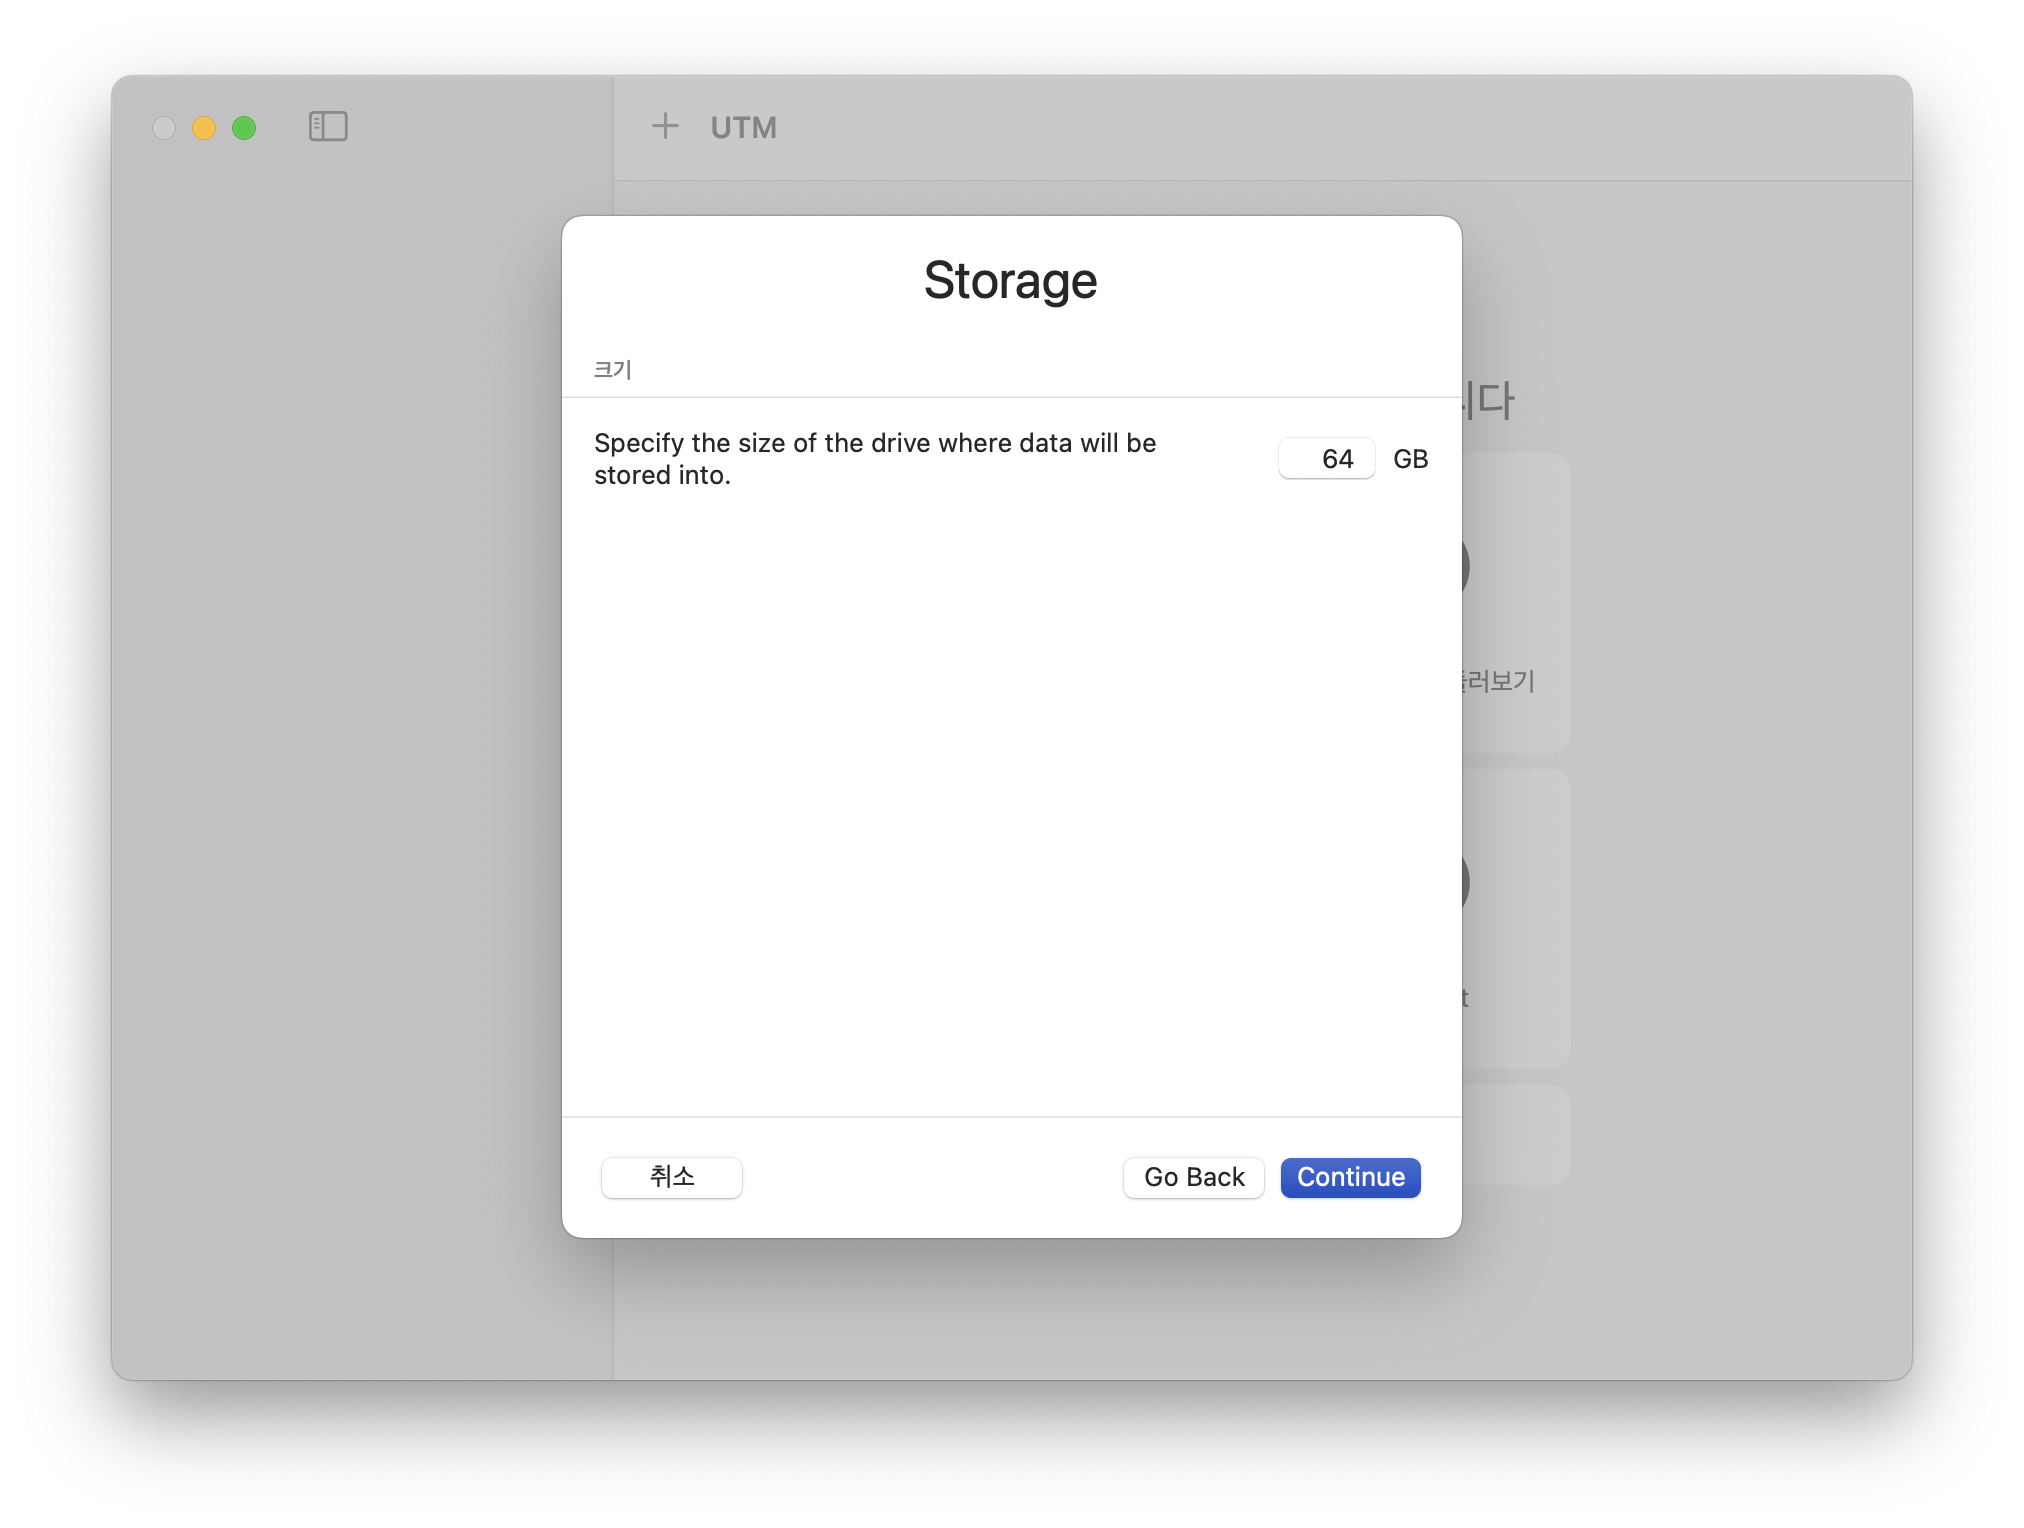
\includegraphics[width=0.9\textwidth]{images/chapter2Images/ch2_image_10.png}
    \caption{Ubuntu 데스크탑 환경}
\end{figure}

\begin{figure}[htbp]
    \centering
    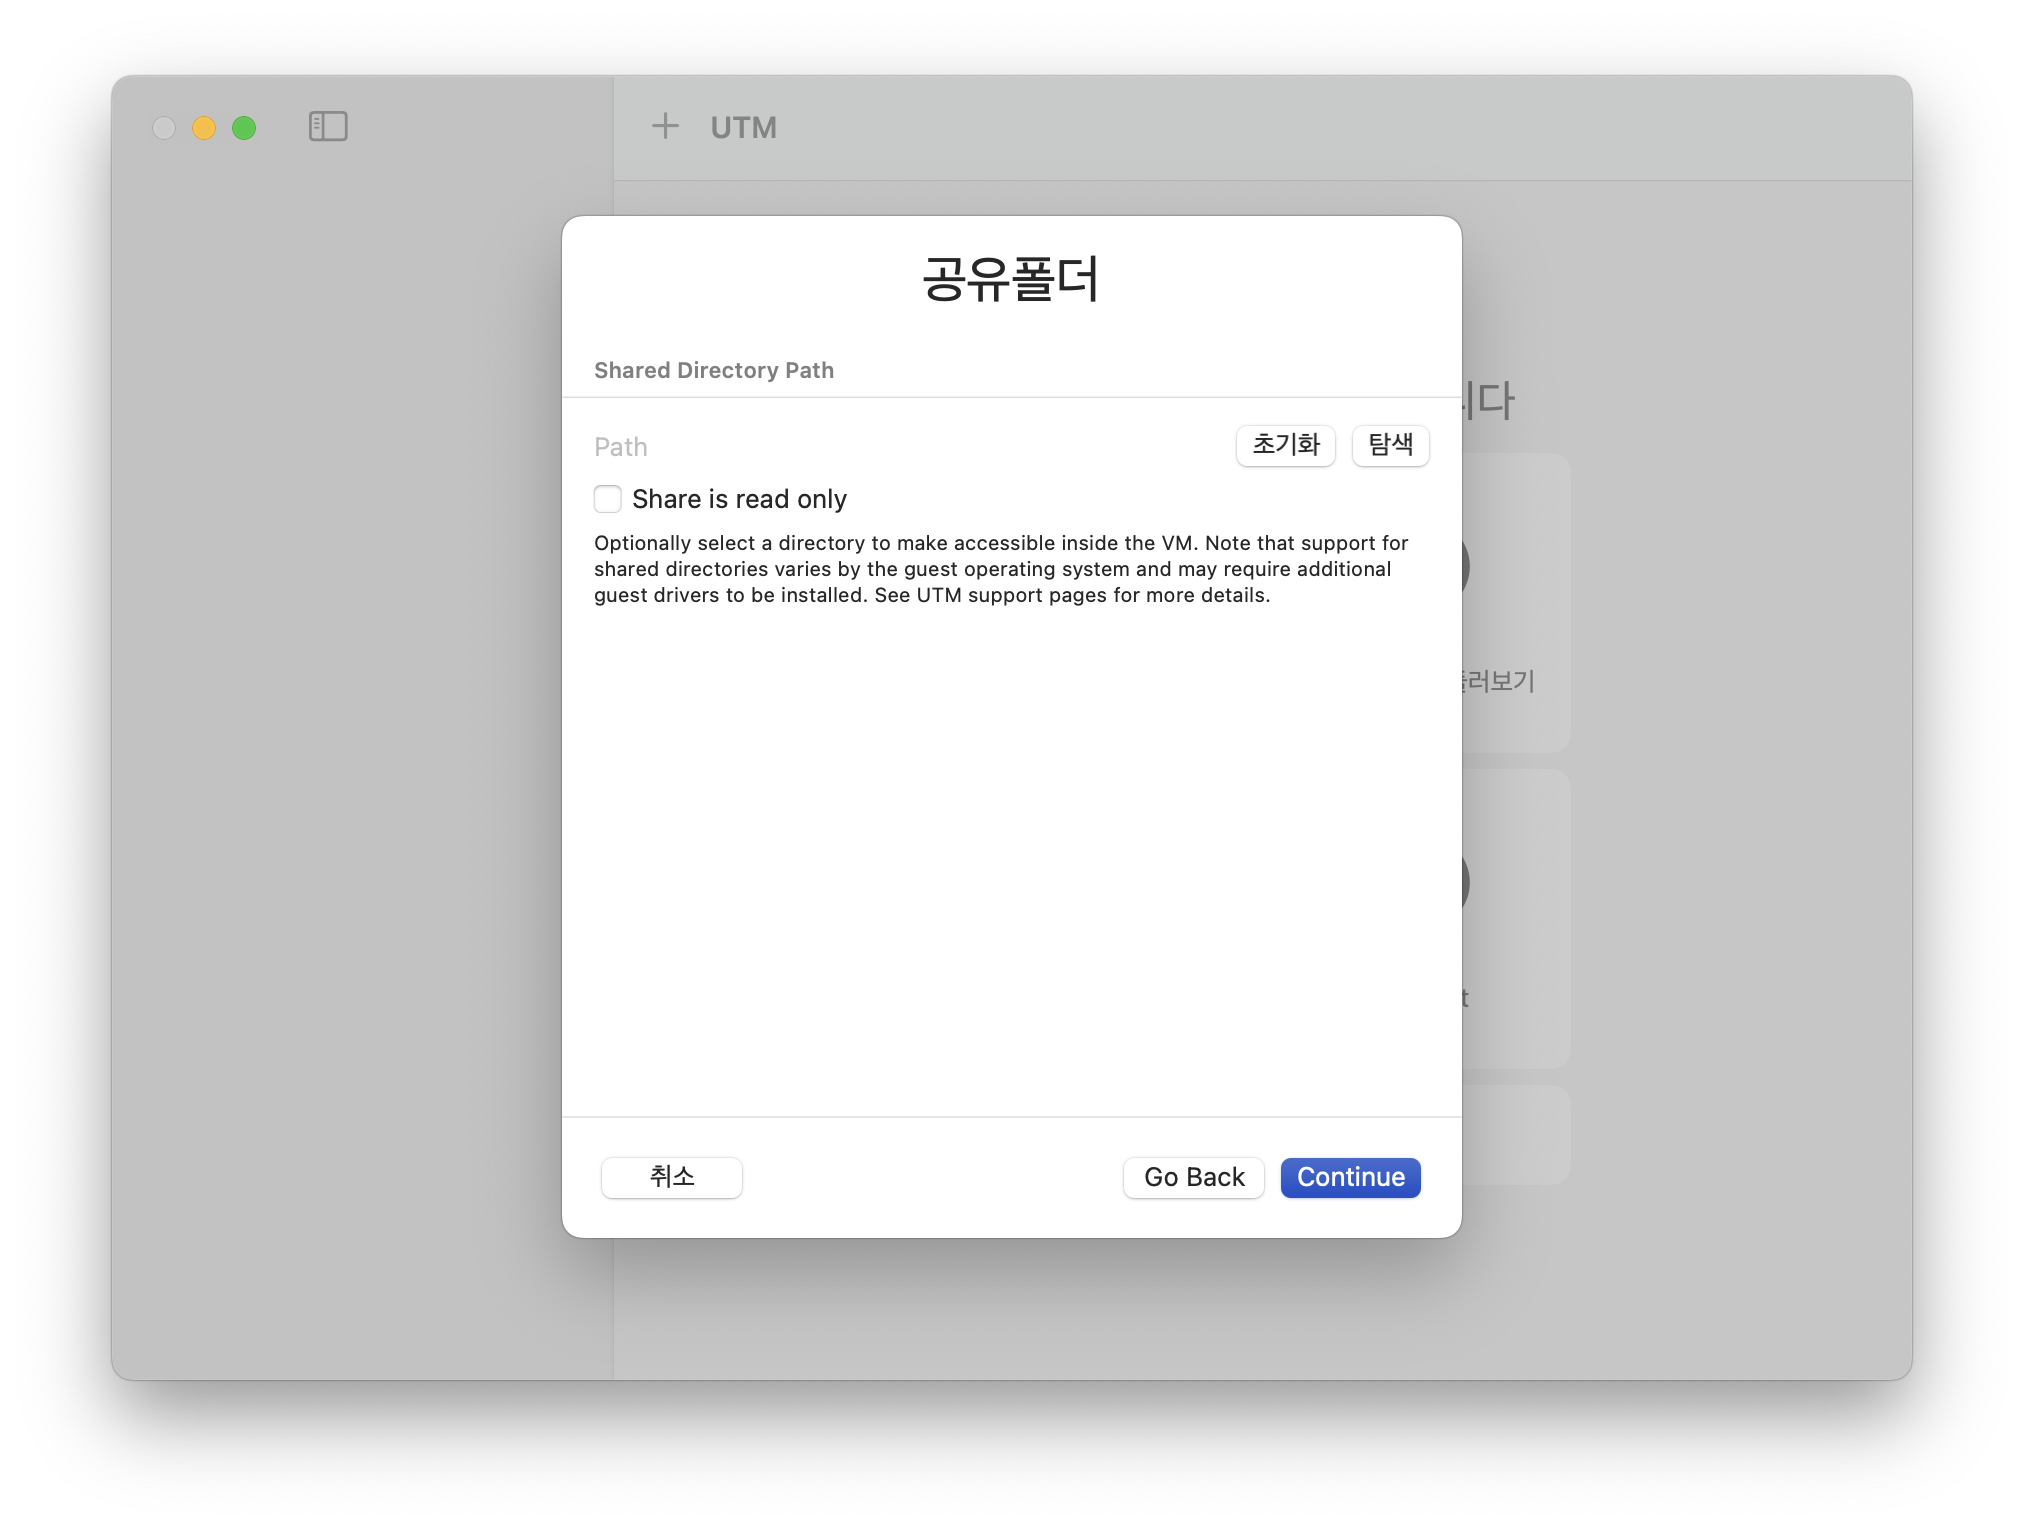
\includegraphics[width=0.9\textwidth]{images/chapter2Images/ch2_image_11.png}
    \caption{사용자 설정}
\end{figure}

\begin{figure}[htbp]
    \centering
    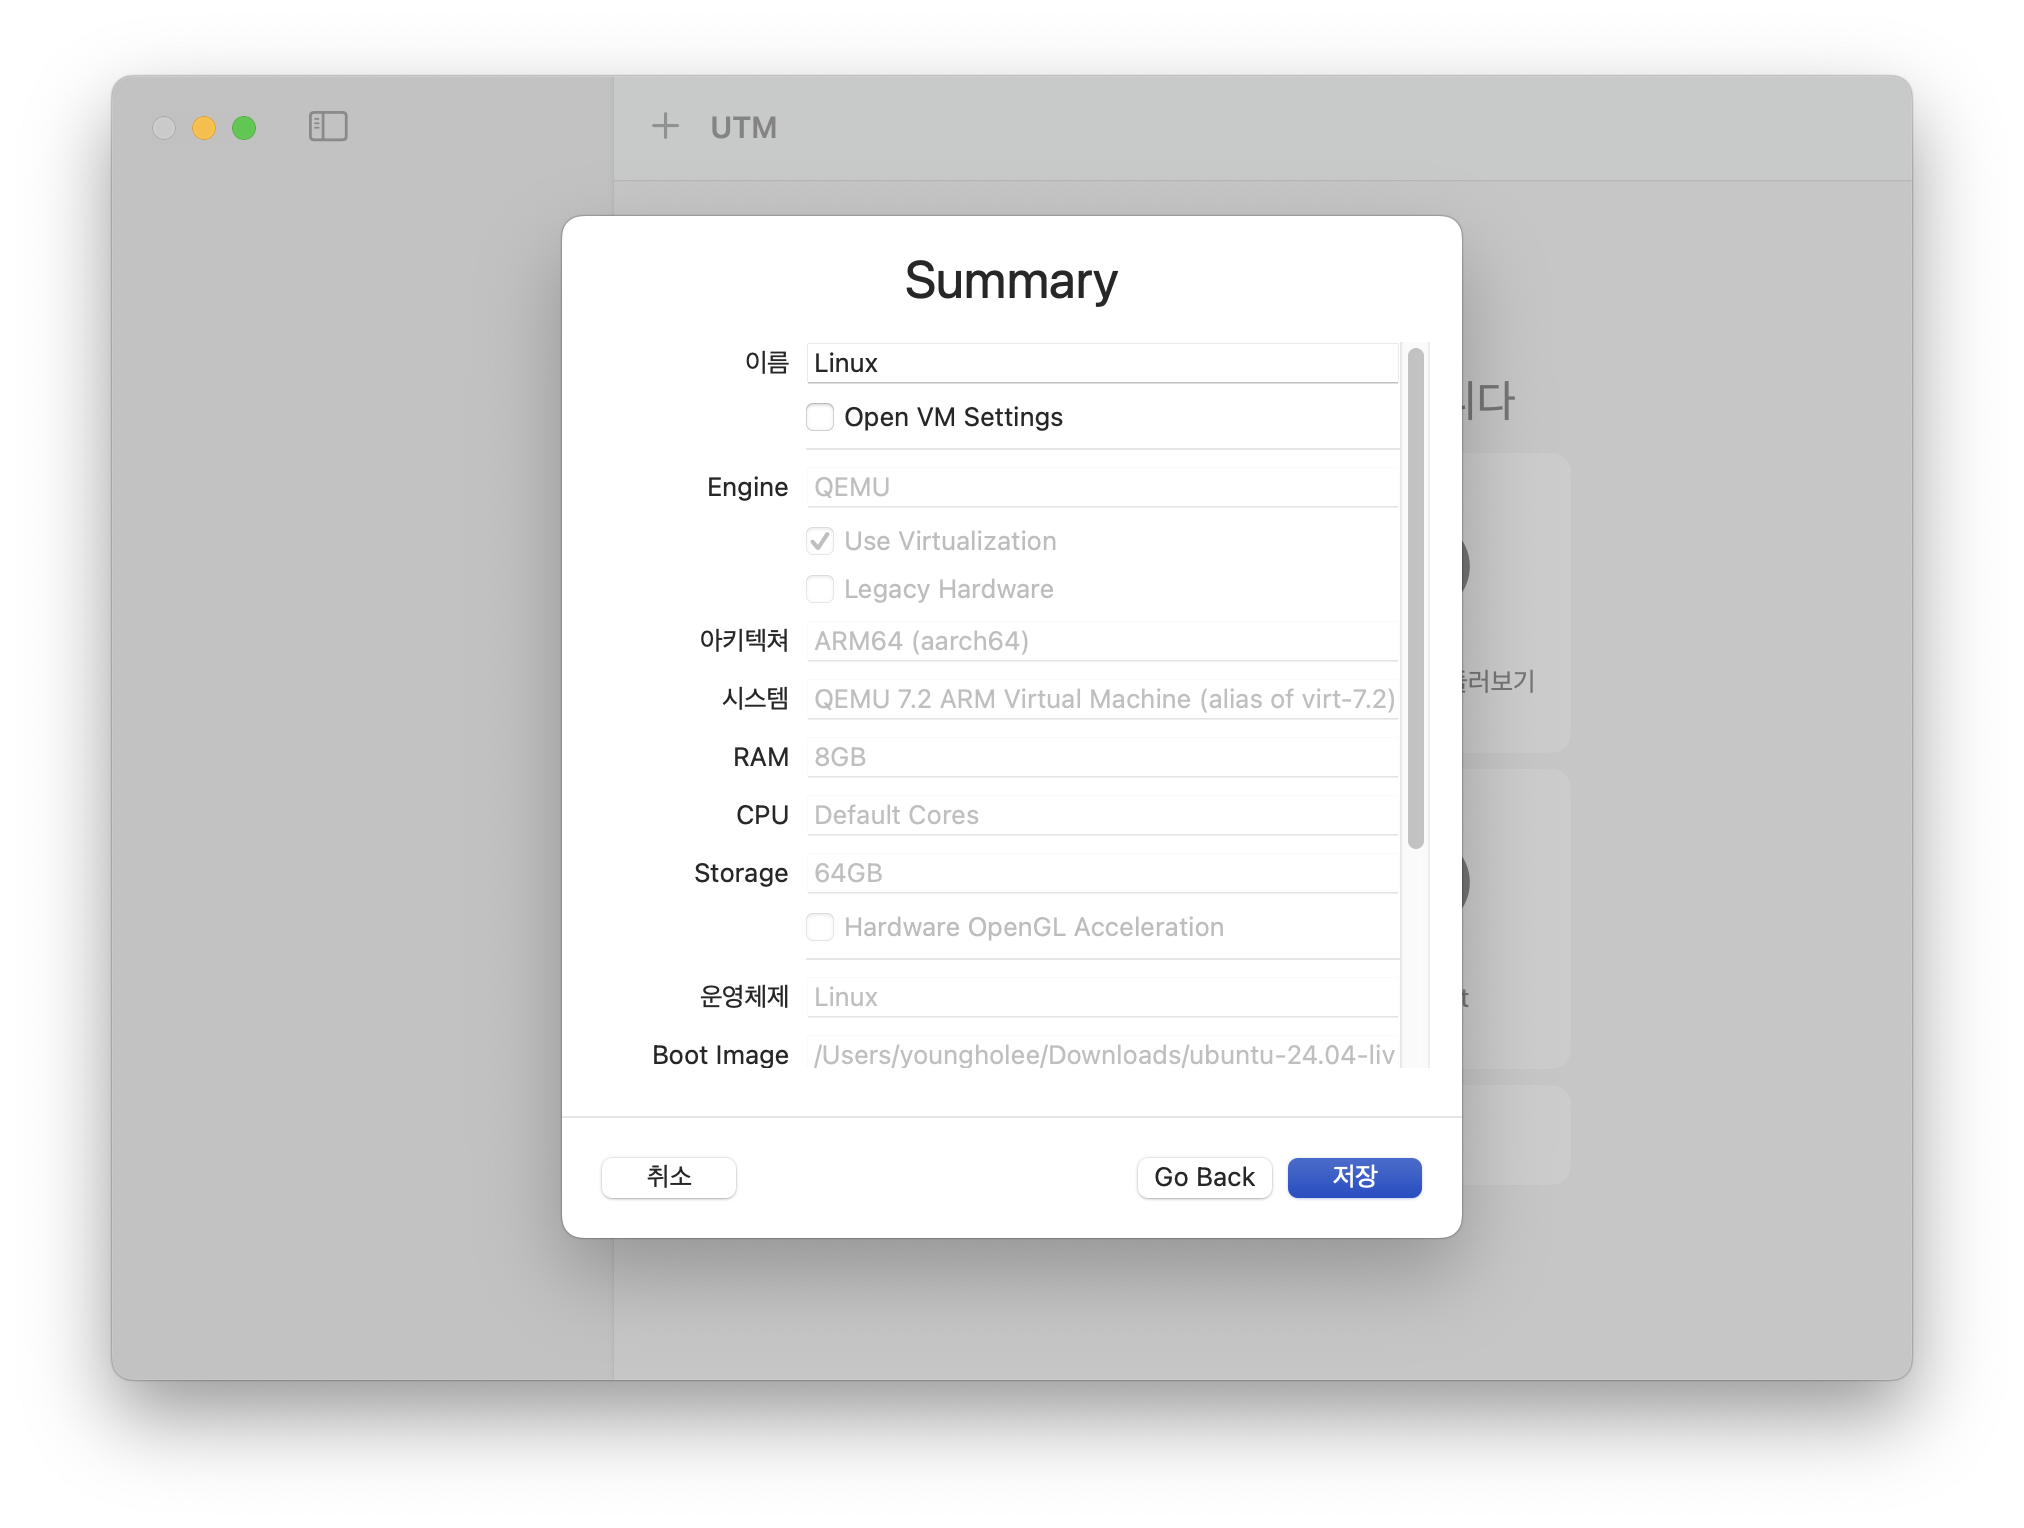
\includegraphics[width=0.9\textwidth]{images/chapter2Images/ch2_image_12.png}
    \caption{업데이트 설치}
\end{figure}

\begin{figure}[htbp]
    \centering
    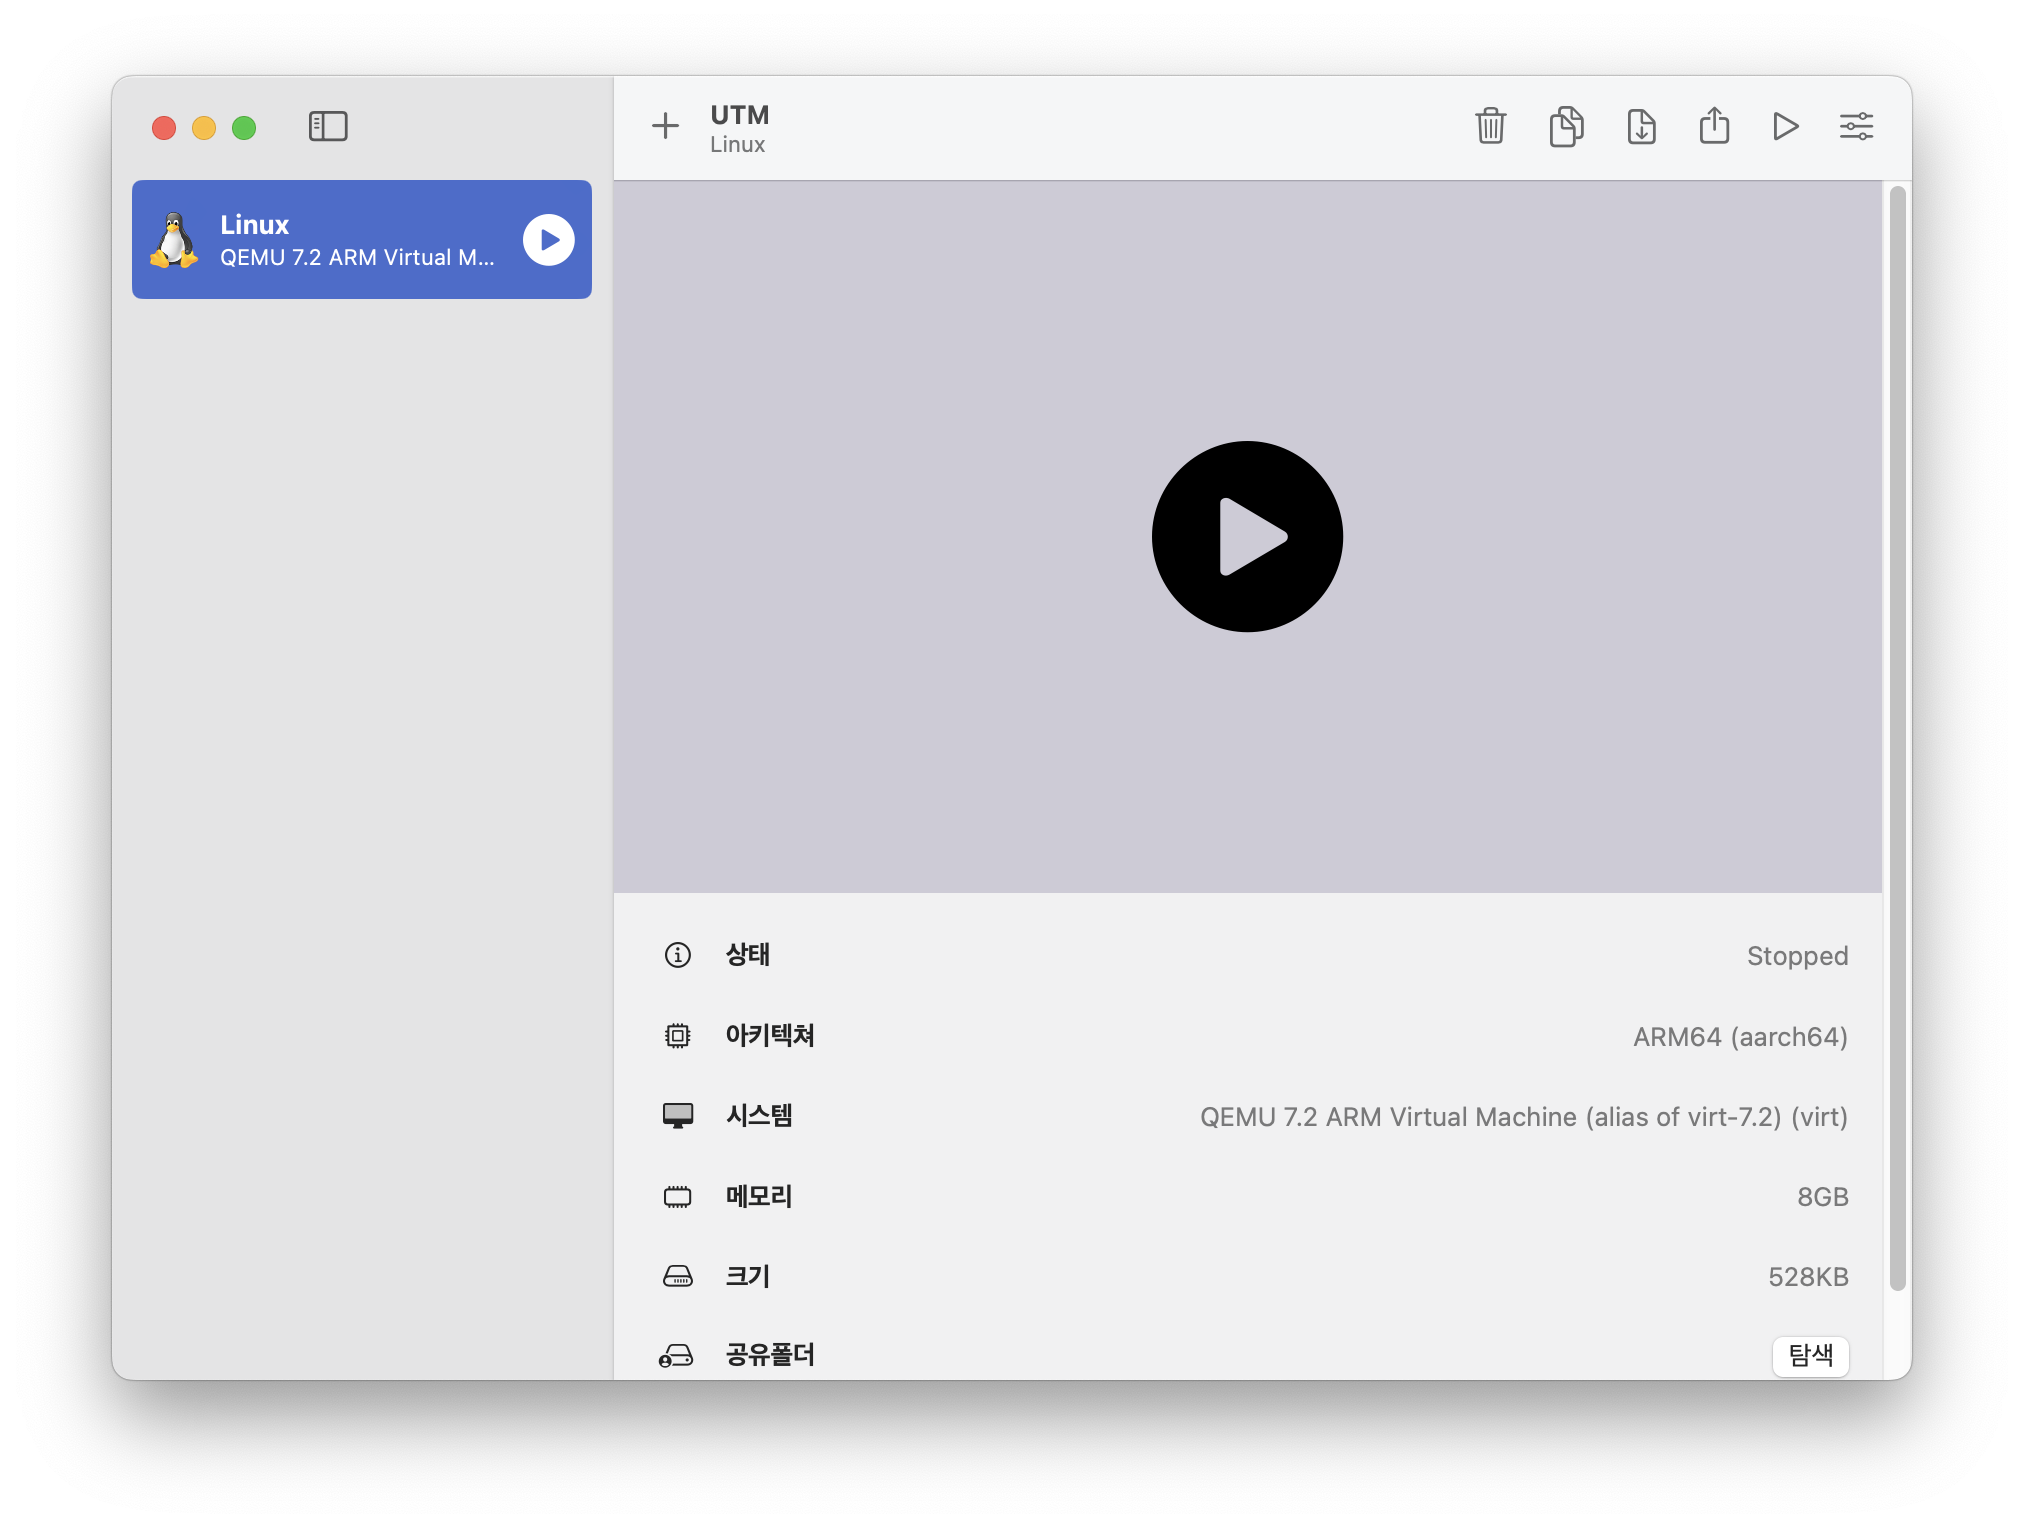
\includegraphics[width=0.9\textwidth]{images/chapter2Images/ch2_image_13.png}
    \caption{시스템 사용 준비 완료}
\end{figure}

\begin{figure}[htbp]
    \centering
    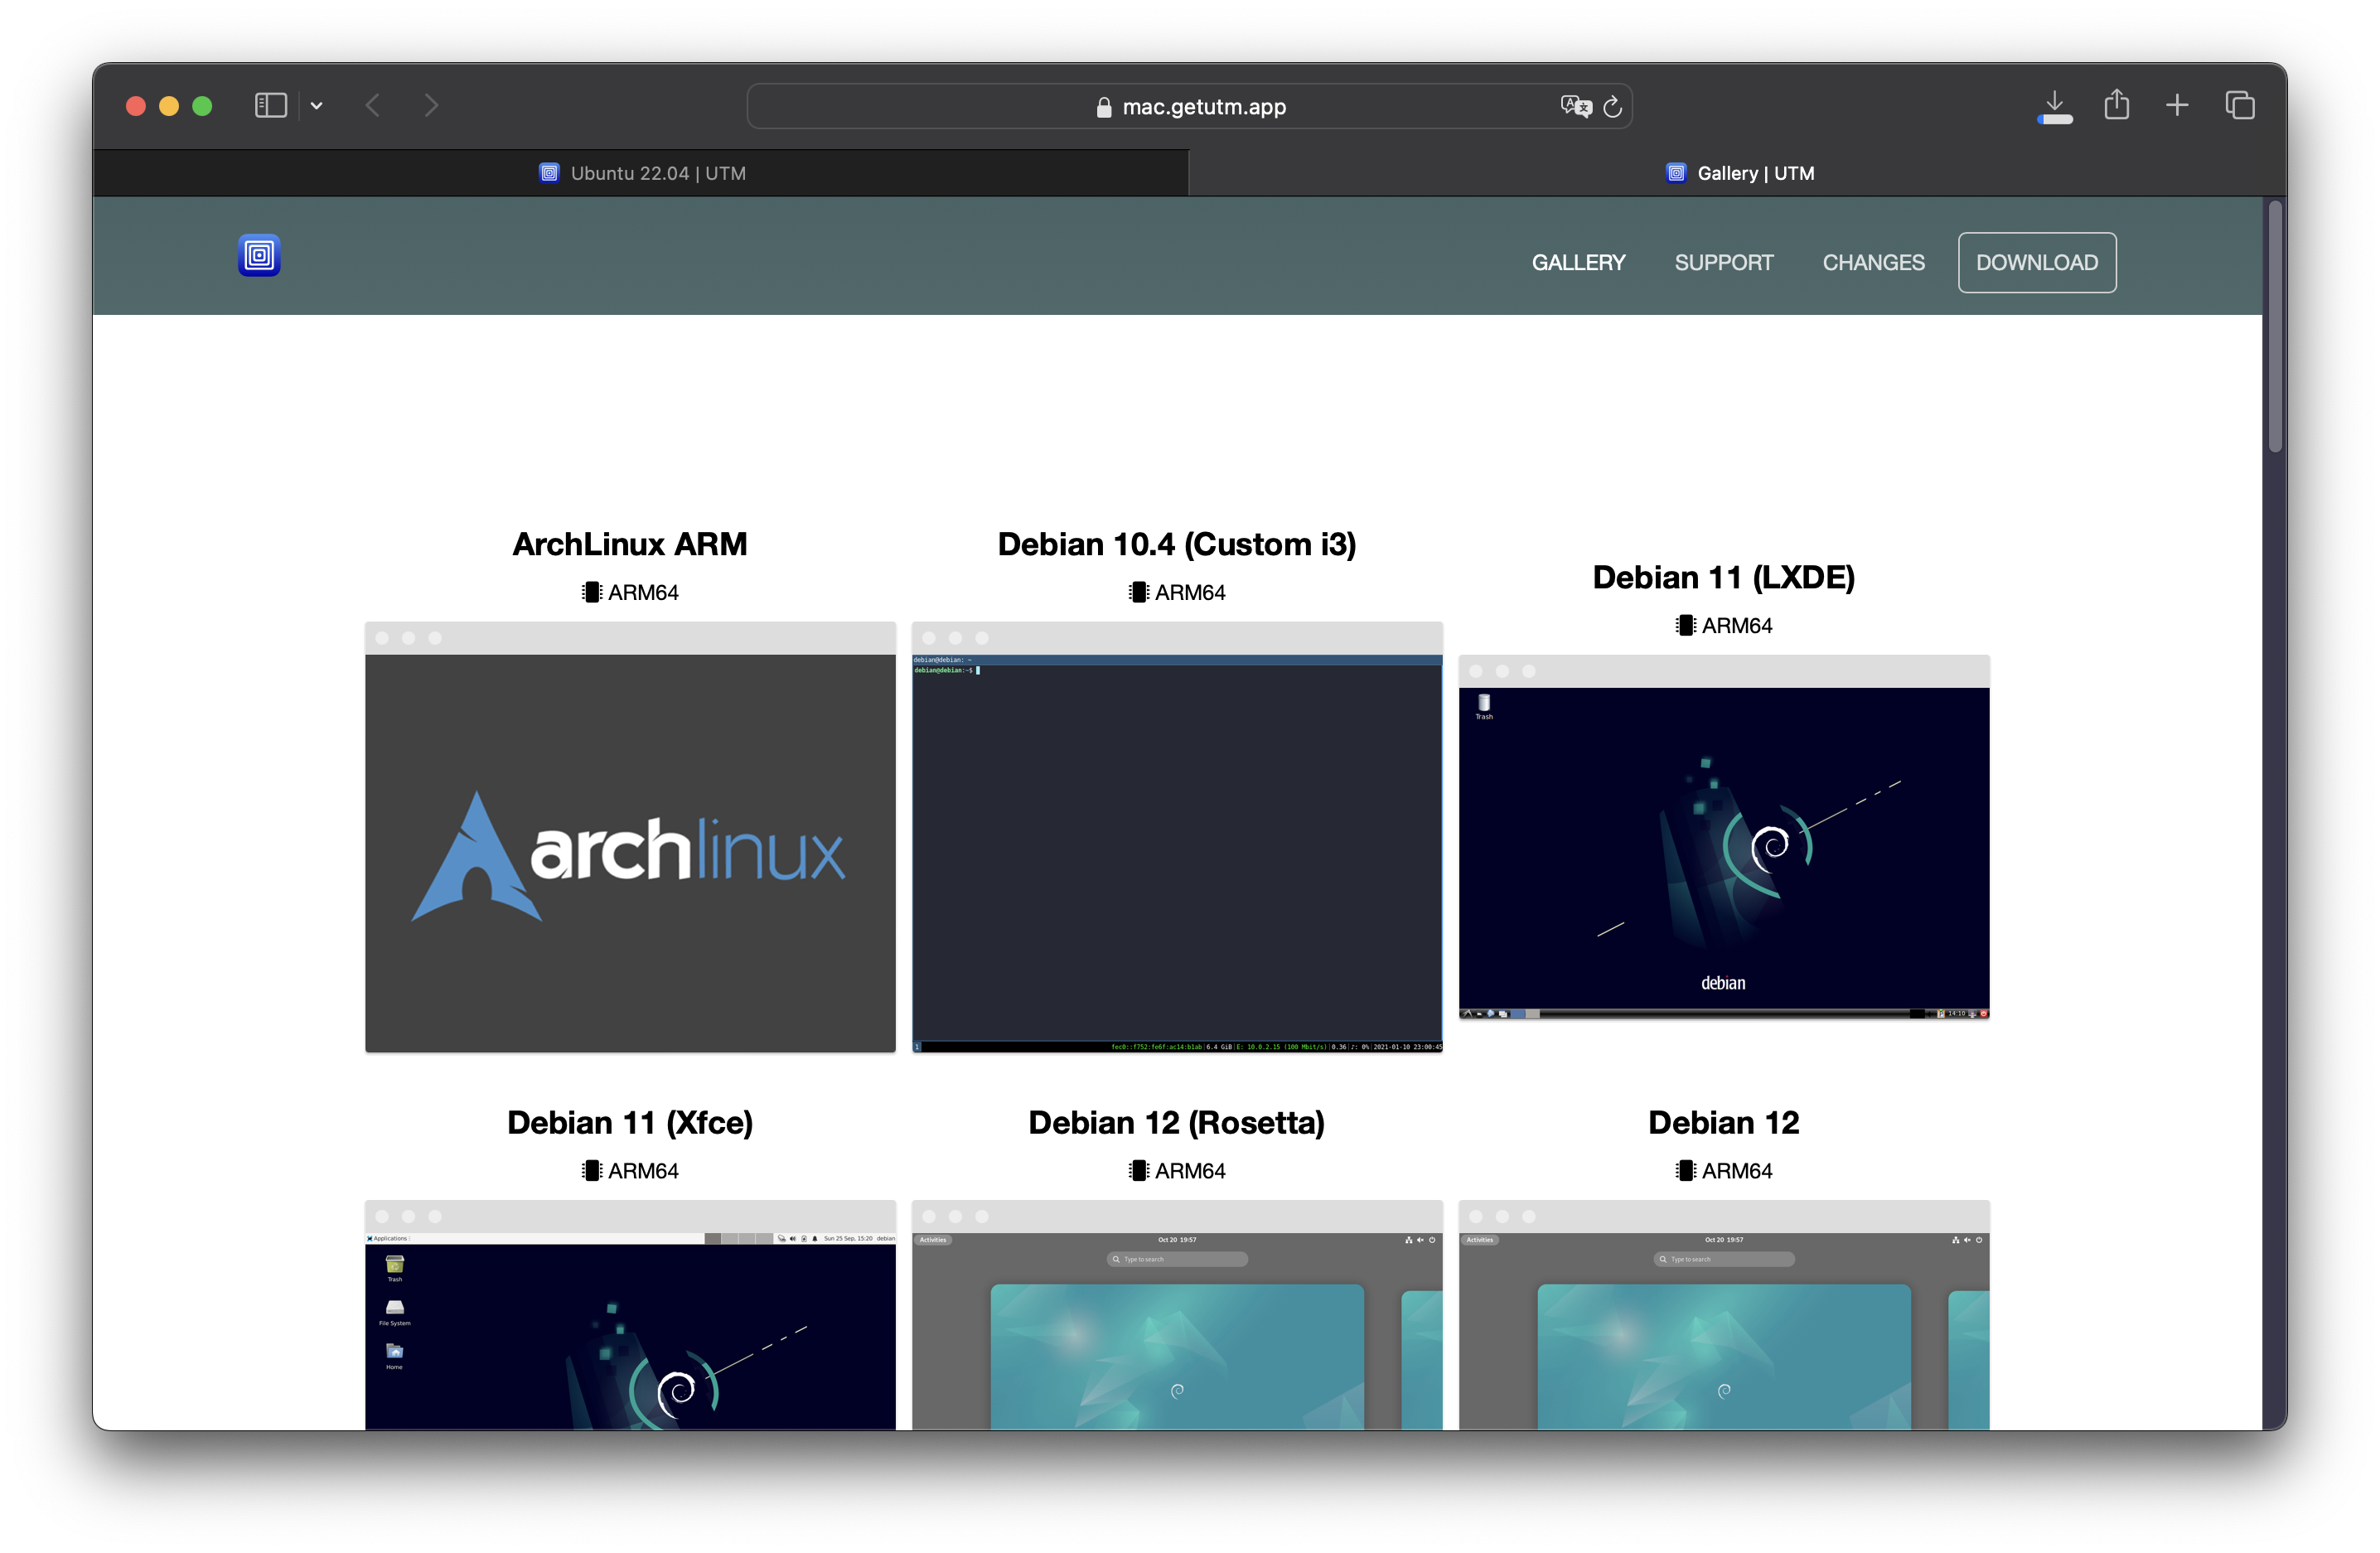
\includegraphics[width=0.9\textwidth]{images/chapter2Images/ch2_image_14.png}
    \caption{첫 번째 응용 프로그램 실행}
\end{figure}

\begin{figure}[htbp]
    \centering
    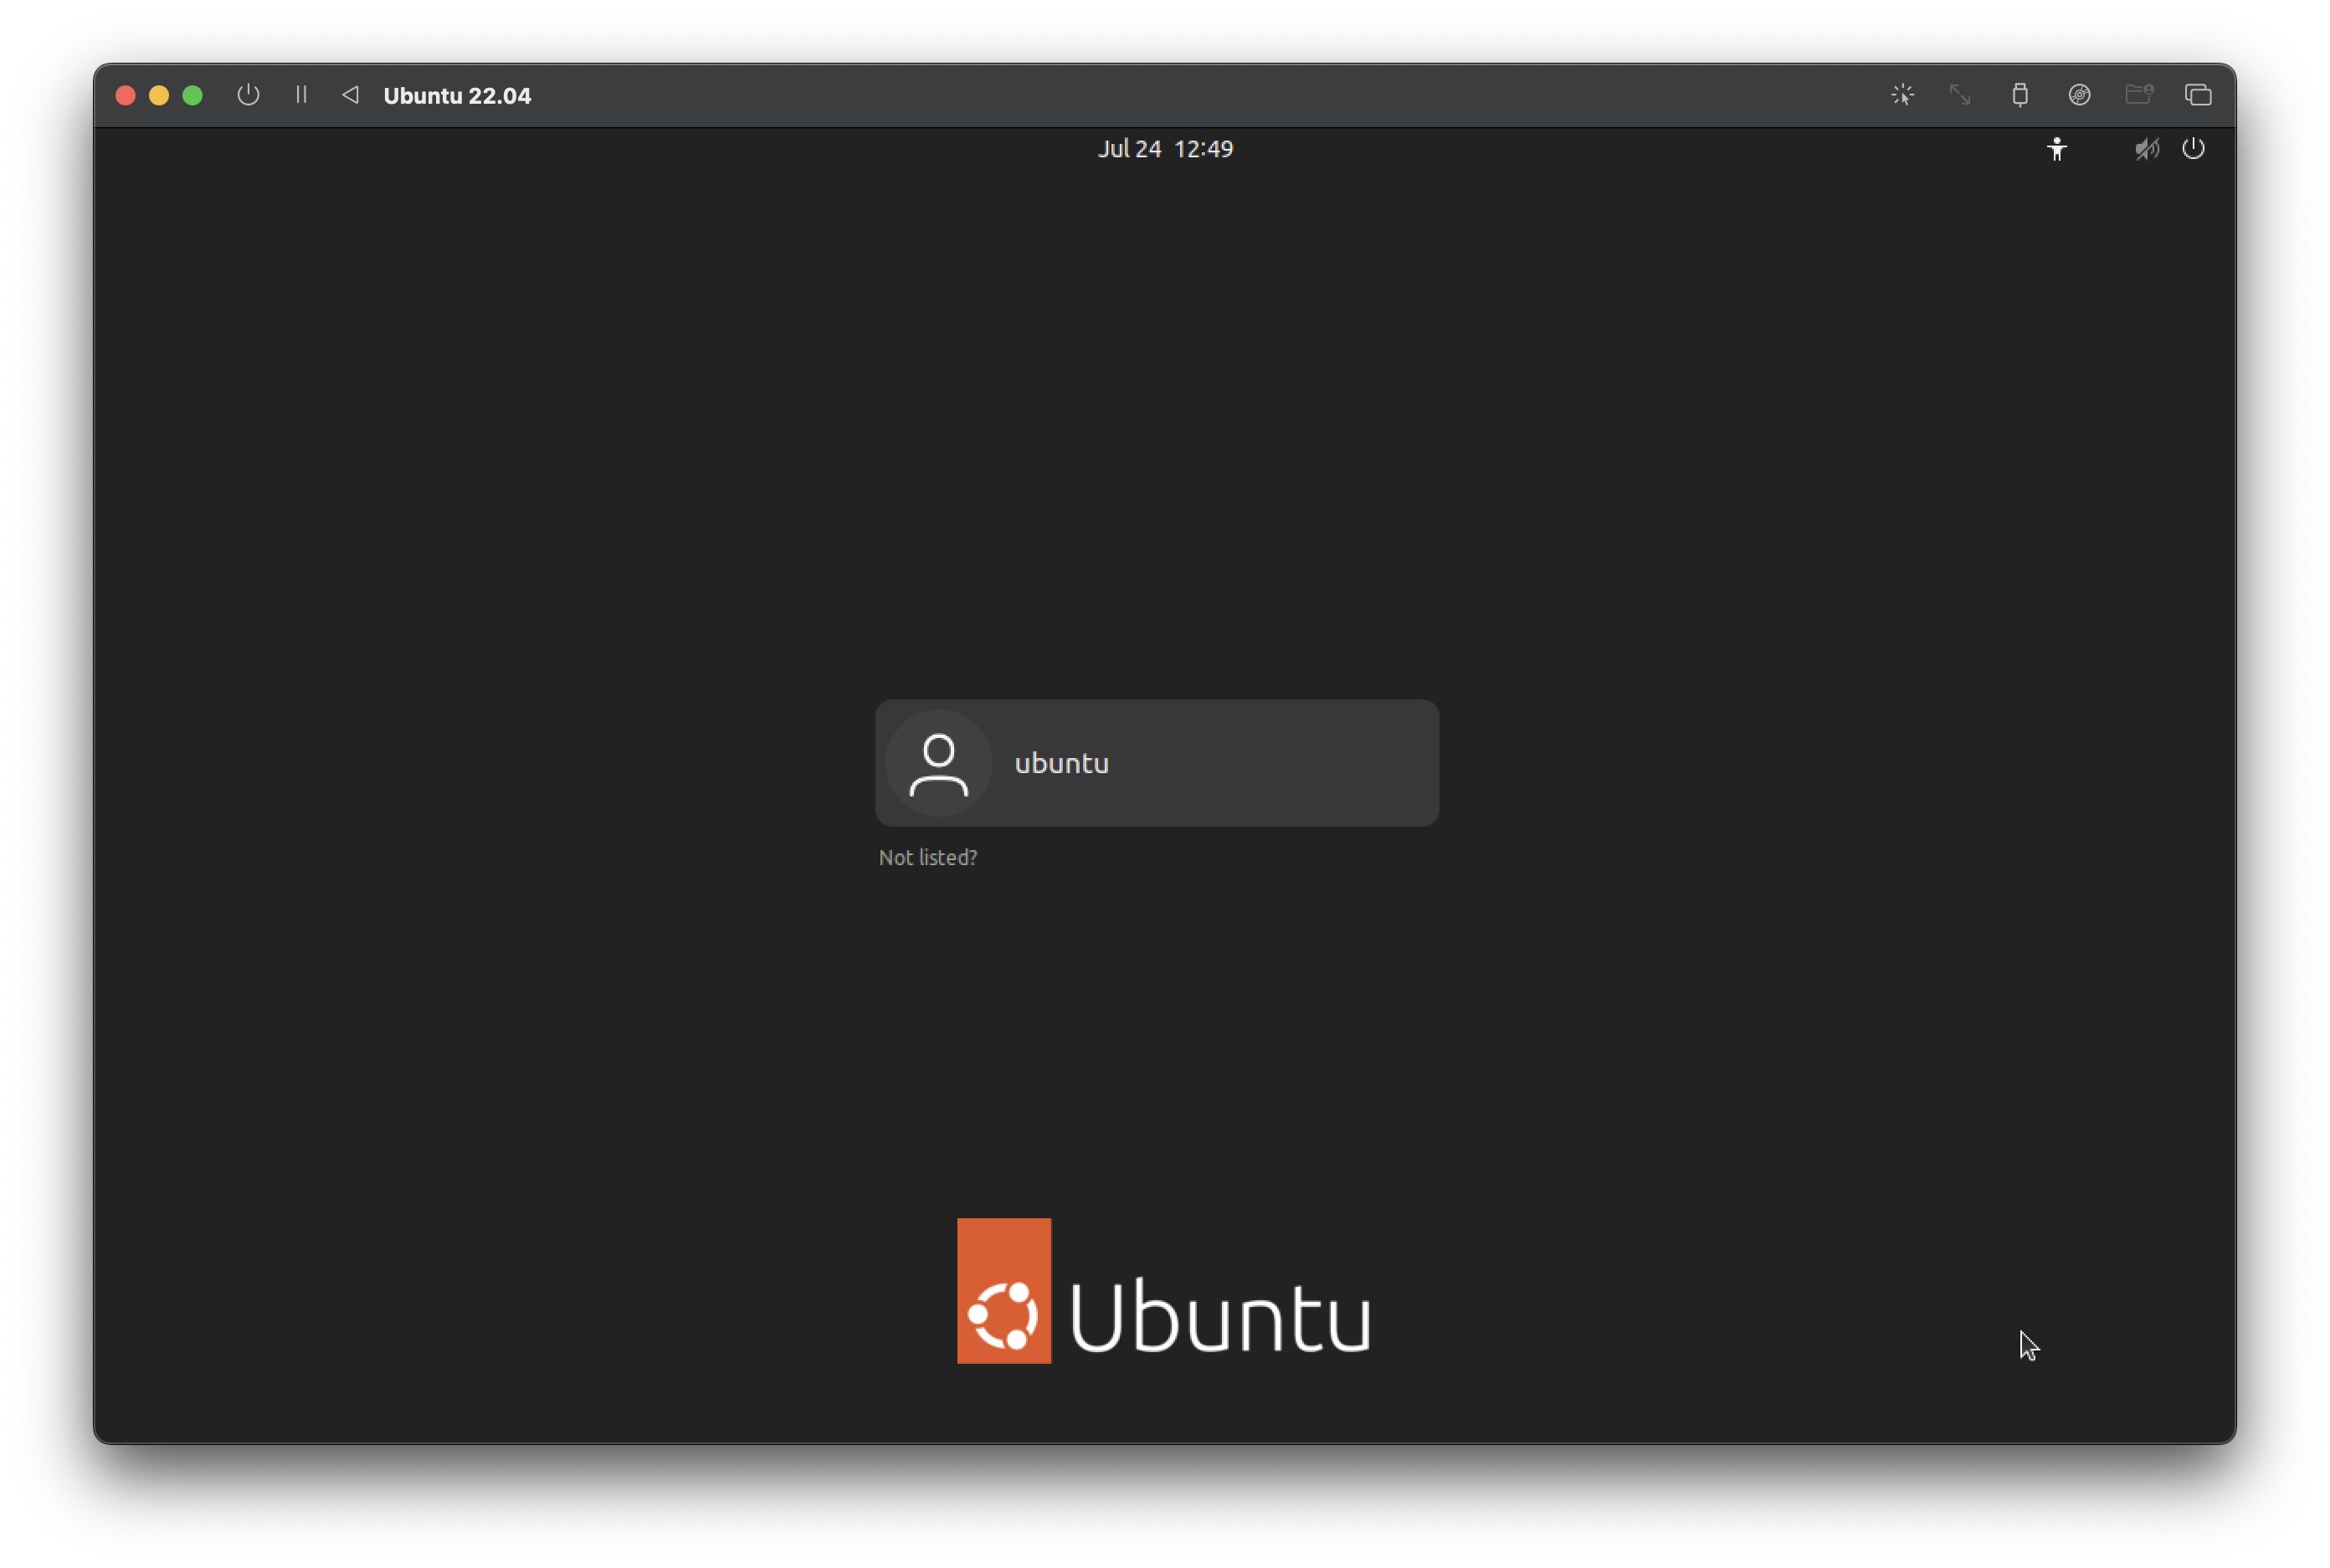
\includegraphics[width=0.9\textwidth]{images/chapter2Images/ch2_image_15.png}
    \caption{Ubuntu 기능 탐색}
\end{figure}

\begin{figure}[htbp]
    \centering
    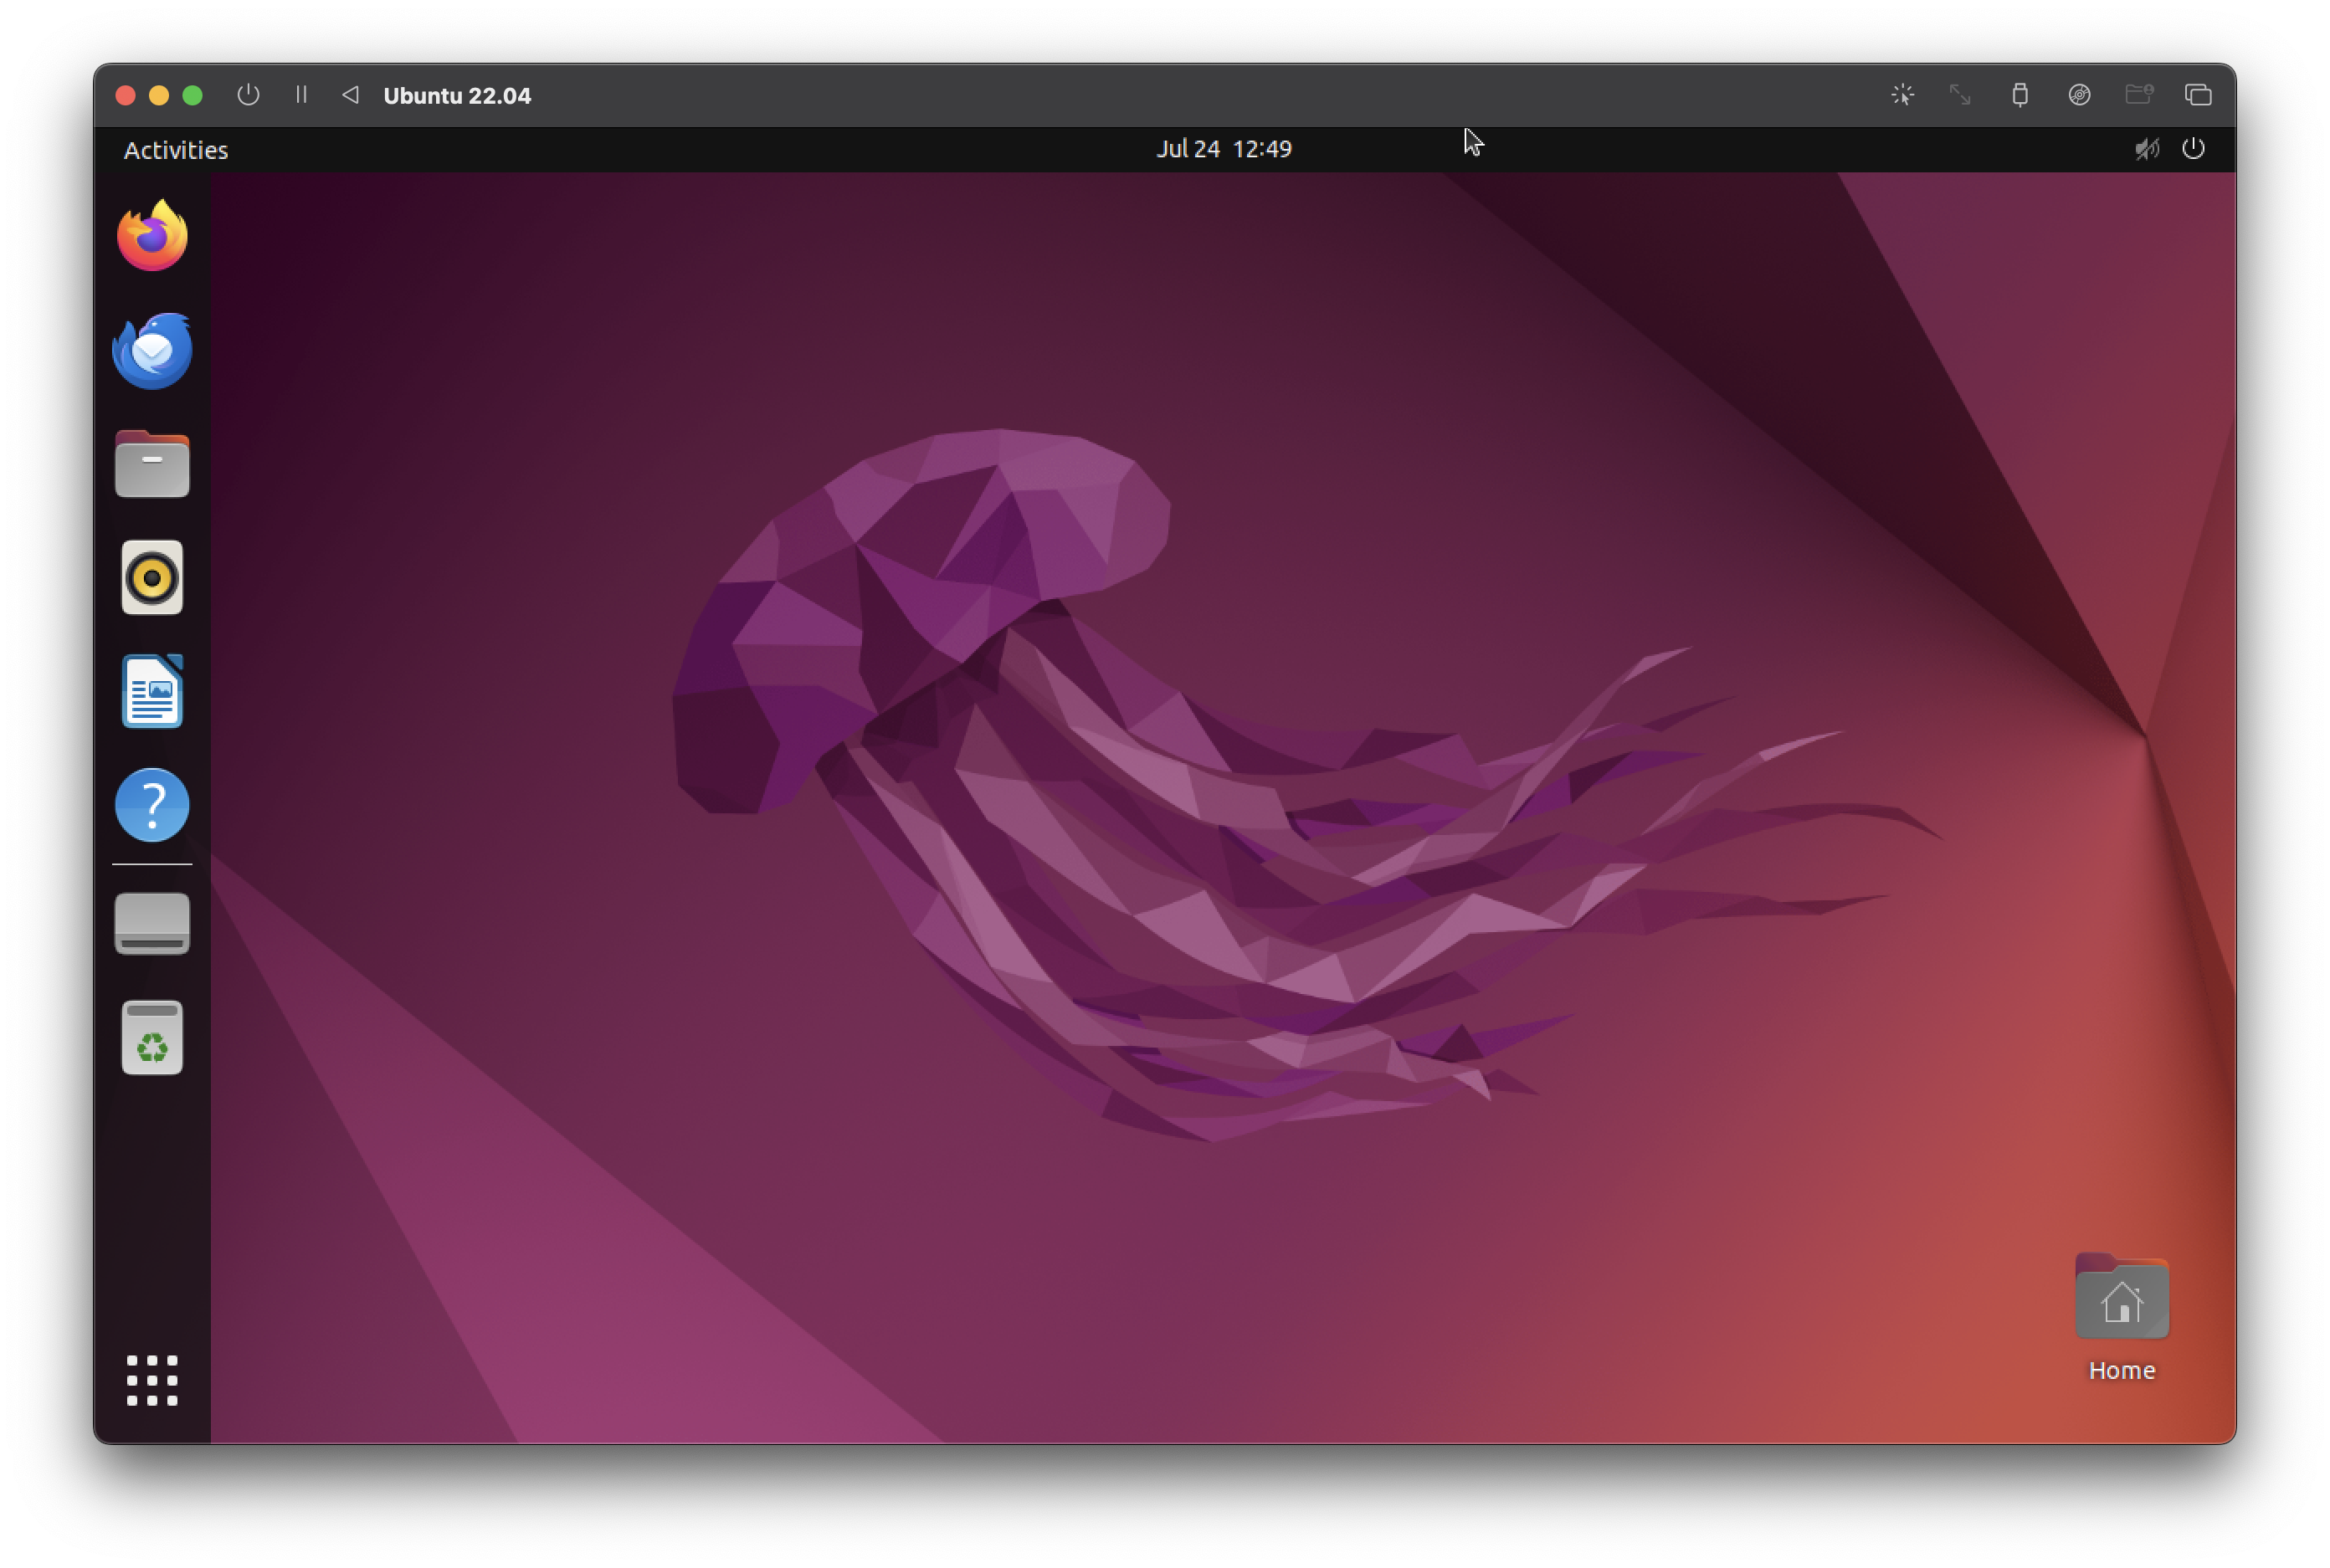
\includegraphics[width=0.9\textwidth]{images/chapter2Images/ch2_image_16.png}
    \caption{Ubuntu 완전 작동}
\end{figure}

\end{document}
